% Defino el tipo de documento
\documentclass[a4paper, 11pts]{article}

% Paquetes usados para el informe
\usepackage[utf8]{inputenc}
\usepackage[spanish]{babel}	
\usepackage{float}
\usepackage{amsmath}

% Estilo del documento
\renewcommand*\familydefault{\sfdefault} 		% Sans Serif as default font
\usepackage[a4paper, 					% Page Layout
                     %showframe,				% This shows the frame
                     includehead,
                     footskip=7mm, headsep=6mm, headheight=4.8mm,
                     top=25mm, bottom=25mm, left=25mm, right=25mm]{geometry}

\setlength{\parindent}{0cm}

\begin{document}

\section{Ejercicio 4: Derivador e Integrador}
En la presente secci\'on se estudiar\'an los circuitos derivador e integrador implementados con amplificador operacionales, analizando su comportamiento, rango de funcionamiento y cualidades o defectos. Adem\'as se presentar\'a un circuito para cada uno de ellos con modificaciones con el fin de mejorar su funcionamiento y se comparar\'an los resultados entre ellos.

Para cada uno de los circuitos, se realiza un an\'alisis te\'orico del mismo y luego se presentan las mediciones y los resultados de las mismas, contrastando o comparando lo observado en la pr\'actica, la simulaci\'on y la teor\'ia.

Adem\'as, todo an\'alisis te\'orico se realiza teniendo en cuenta que los circuitos son armados empleando una resistencia $R = 5k \Omega$, un capacitor $C = 20nF$ y un amplificador operacional LM833 cuyos par\'ametros son:
\begin{itemize}
	\item $A_{vol} = 100000$
	\item $f_p = 150Hz$
	\item $GBP = 15MHz$
	\item $SR = 7 \frac{V}{\mu s}$
	\item $r_{id} = 175k \Omega$
	\item $Z_o = 37 \Omega$
\end{itemize}

<<<<<<< HEAD
	\subsection{Circuito derivador}
 
\subsubsection{An\'alisis Te\'orico}

\begin{figure}[H]
	\centering
	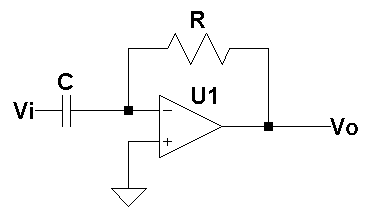
\includegraphics[scale=0.8]{Recursos/Derivador/Circuito_derivador.png}
	\caption{Circuito derivador}
	\label{fig:circuito_derivador}
\end{figure}

=======

	\subsection{Circuito derivador}
 
\subsubsection{An\'alisis Te\'orico}

\begin{figure}[H]
	\centering
	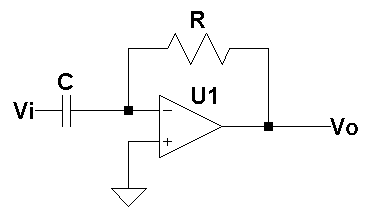
\includegraphics[scale=0.8]{Recursos/Derivador/Circuito_derivador.png}
	\caption{Circuito derivador}
	\label{fig:circuito_derivador}
\end{figure}

>>>>>>> 1c903573e405a1b067e44751a5fd15495a8566b3
\paragraph*{Funci\'on transferencia en condiciones ideales}se busca la funci\'on de transferencia del circuito bajo condiciones ideales, esto es, asumiendo que el amplificador operacional no tiene variaci\'on en su ganancia de lazo abierto con la frecuencia y que la misma tiende a infinito, $A_{vol} \to \infty$. En este marco de idealidad, las impedancias de entrada y salida del amplificador operacional son $Z_{in} \to \infty$ y $r_o = 0$. Para este c\'alculo se conoce la ganancia ideal de un amplificador inversor y se asume al mismo un sistema LTI, causal y bibo-estable.

\begin{equation}
	H(s) = \frac{V_o}{V_i} = \frac{-R}{ \frac{1}{s \cdot C}} = -s \cdot R  \cdot C
	= -\frac{s}{10000}
	\label{eq:derivador_transfer_ideal}
\end{equation}

Se puede observar que por la propiedad de la derivada para transformada de Laplace, multiplicar por la variable $s$ en tal dominio, implica derivar la se\~nal en el dominio temporal, de forma tal que se puede llegar:

\begin{equation*}
	V_o(s) = V_i(s) \cdot H(s) = V_i(s) \cdot -sRC \Rightarrow
	Vo(t) = -RC \cdot \frac{\delta V_i(t)}{\delta t}
\end{equation*}

Otra observaci\'on sobre la funci\'on de transferencia ideal, es que para frecuencias altas, 
seg\'un la magnitud de la se\~nal de entrada, se puede producir la saturaci\'on del amplificador
operacional pues la ganancia es muy elevada y la salida supera el valor de la fuente de 
alimentaci\'on del circuito. Por otro lado, el sistema descripto por dicha funci\'on de 
transferencia ideal, no es bibo-estable como se asumi\'o desde el principio. 
Esto se obtiene del hecho de que la antitransformada de la funci\'on transferencia, es decir la respuesta impulsiva, 
es la derivada del delta de dirac. Ergo, para se\~nales acotadas en la entrada, la operaci\'on de derivar
puede dar como resultado, en algunos casos, una se\~nal de salida no acotada.

%TODO Agregar diagrama de polos y ceros aca!

\paragraph*{Funci\'on transferencia con $A_{vol}$ finito}se considera que $A_{vol}$ es finito con lo cual se lo debe tener en cuenta, y para llegar a la funci\'on transferencia se plantea por un lado la superposici\'on de las tensiones sobre las entradas del amplificador operacional y luego la expresi\'on de salida del mismo para obtener:

\begin{equation*}
	v^{-} = \frac{V_i \cdot R}{\frac{1}{sC} + R} + \frac{V_o \cdot \frac{1}{sC}}{\frac{1}{sC} + R}
	= \frac{V_i \cdot s \cdot R \cdot C + V_o}{1 + s \cdot R \cdot C}
\end{equation*}

\begin{align*}
	V_o = (v^{+} - v^{-}) \cdot A_{vol}
	= - \frac{V_i \cdot s \cdot R \cdot C + V_o}{1 + s \cdot R \cdot C} \cdot A_{vol} \\
	V_o \cdot \left[ 1 + \frac{A_{vol}}{1 + s \cdot R \cdot C} \right]
	= - \frac{V_i \cdot s \cdot R \cdot C \cdot A_{vol}}{1 + s \cdot R \cdot C}
\end{align*}
\begin{equation}
	H(s) = \frac{V_o(s)}{V_i(s)} = \frac{\frac{s \cdot A_{vol} \cdot RC}{A_{vol} + 1}}{1 + \frac{s}{\frac{A_{vol} + 1}{R \cdot C}}}
	= - \frac{\frac{s}{2 \pi \cdot 1,591kHz}}{1 + \frac{s}{2 \pi \cdot 159,15MHz}}
	\label{eq:derivador_transfer_avol_finito}
\end{equation}

De esto \'ultimo se puede observar que aparece, a diferencia de antes, un polo adicional que podr\'ia ser despreciado o incluso anulado bajo las condiciones de idealidad previamente analizadas. Es importante destacar de esta nueva funci\'on de transferencia que si se obtiene la frecuencia de corte donde se ubica este polo y limitamos el rango de funcionamiento una decada antes del mismo, podemos considerar condiciones de idealidad tal que el derivador podr\'ia seguir funcionando como tal. Esto tambi\'en se puede ver considerando que, si se llama $\omega_o = \frac{(A_{vol} + 1)}{R \cdot C}$ a la frecuencia angular de corte:
\begin{equation*}
	Si, s << \frac{\omega_o}{10} \Rightarrow 1 >> \frac{s}{\omega_o} \Rightarrow 
	H(s) \approx - \frac{s \cdot A_{vol} \cdot RC}{A_{vol} + 1} \approx
	- s \cdot R \cdot C
\end{equation*}

En primera instancia, este nuevo polo que ha de aparecer establece como se dijo antes un l\'imite superior hasta el
cual puede considerarse que el comportamiento del sistema es ideal. No obstante, por otro lado este aspecto puede resultar beneficioso
en t\'erminos de estabilidad, pues a diferencia de un derivador ideal, a altas frecuencias la ganancia no sigue aumentando.

%TODO Agregar diagrama de polos y ceros aca!

\paragraph*{Funci\'on transferencia con polo dominante} tomando en cuenta el polo dominante 
que el fabricante del amplificador operacional coloca a una baja frecuencia para 
que el ruido se vea atenuado en las altas frecuencias, pues es donde saldr\'ia en contrafase
<<<<<<< HEAD
y producir\'ia una realimentaci\'on positiva. Entonces reemplazado la ecuaci\'on \ref{eq:derivador_polo_dominante} 
=======
y producir\'ia una realimentaci\'on positiva. Entonces reemplazado la ecuaci\'on \ref{eq:polo_dominante} 
>>>>>>> 1c903573e405a1b067e44751a5fd15495a8566b3
en la ecuaci\'on \ref{eq:derivador_transfer_avol_finito} y operando:

\begin{equation}
	A_{vol}(\omega) = \frac{A_o}{1 + \frac{s}{\omega_p}}
	\label{eq:derivador_polo_dominante}
\end{equation}

\begin{equation}
	H(s) = - \frac{s \cdot A_{o} \cdot R \cdot C}{(1 + s \cdot C \cdot R) \cdot (1 + \frac{s}{\omega_p}) + A_{o}} = - \frac{R \cdot C \cdot A_{o}}{A_{o} + 1} \cdot \frac{s}{1 + s \cdot \frac{1 + \omega_p \cdot RC}{\omega_p \cdot(A_o + 1)} + s^{2} \cdot \frac{RC}{\omega_p \cdot (A_o + 1)}}
\end{equation}

En esta \'ultima condici\'on se puede observar que el circuito se comporta
como un segundo orden por ser de segundo grado en el denominador, 
para lo cual es necesario determinar algunos par\'ametros que permitan
establecer cu\'al es el comportamiento de tal sistema y para ello se 
despejan de las siguientes expresiones los valores de $\xi$ y $\omega_o$.

\begin{equation*}
	\omega_o^{2} = \frac{\omega_p \cdot (A_o + 1)}{RC} \Rightarrow \omega_o = \sqrt{\frac{\omega_p \cdot (A_o + 1)}{RC}}	
\end{equation*}

\begin{equation*}
	\frac{2 \cdot \xi}{\omega_o} = \frac{(1 + \omega_p \cdot R \cdot C)}{\omega_p \cdot(A_o + 1)}
	\Rightarrow \xi = \frac{1}{2} \cdot \frac{1 + \omega_p \cdot R \cdot C}{\sqrt{\omega_p \cdot R \cdot C \cdot (A_o + 1)}}
\end{equation*}

\begin{equation}
	H(s) = - \frac{\frac{s}{2 \pi \cdot 1,591kHz}}
	{1 + s \cdot 11,53 \cdot 10^{-9} + \left( \frac{s}{2 \pi \cdot 154,51kHz} \right)^{2}}
	\label{eq:derivador_transfer_polo_dominante}
\end{equation}

Finalmente, se obtiene que $\omega_o = 970817,81 \frac{1}{s}$ y $\xi = 0,0056357$. Esto \'ultimo indica que la respuesta natural del sistema durante una transici\'on entre estados estables contiene un subamortiguamiento, pero m\'as importante, que los polos son complejos y conjugados donde la frecuencia de corte est\'a en $f_o = 154,51kHz$ y presenta un sobrepico.

Para ubicar a qu\'e frecuencia y con qu\'e magnitud ocurre este pico en la respuesta en frecuencia, se busca el m\'inimo de la funci\'on del denominador de la respuesta en frecuencia en m\'odulo. Vale mencionar que al igual que para los futuros an\'alisis que se hagan, se asume el sistema LTI, causal y bibo-estable con lo que luego se puede evaluar $s = j \omega$ para encontrar la respuesta en frecuencia a partir de la funci\'on transferencia.
Llamando $D(s)$ a la expresi\'on del denominador de la funci\'on transferencia, se busca el m\'inimo del m\'odulo de tal funci\'on.

\begin{equation*}
	D(s) = \left( \frac{s}{\omega_o} \right)^{2} + \frac{2 \cdot \xi}{\omega_o} \cdot s + 1
	\Rightarrow
	D(w) = \frac{j \cdot 2 \cdot \xi \cdot \omega}{\omega_o} + \left( \frac{\omega_o^{2} - \omega^{2}}{\omega_o^{2}} \right)
\end{equation*}

\begin{equation*}
	|D(w)| = \sqrt{\left( \frac{2 \xi \omega}{\omega_o} \right)^{2} + \left( \frac{\omega_o^{2} - \omega^{2}}{\omega_o^{2}} \right)^{2}}
\end{equation*}

\begin{equation}
	\frac{\delta |D(w)|}{\delta w}
	= 0 \Leftrightarrow 2 \cdot \xi^{2} \cdot \omega - \frac{\omega \cdot (\omega_o^{2} - \omega^{2})}{\omega_o^{2}} = 0
	\Leftrightarrow
	\omega = \omega_o \cdot \sqrt{1 - 2 \cdot \xi^{2}}
\end{equation}

Entonces, el pico dentro de la respuesta en frecuencia caracter\'istico de este sistema se puede encontrar, te\'oricamente, en la frecuencia $\omega_{pico} = 970817,8 \cdot \sqrt{1- 2 \cdot (0,0056)^{2}} = 970786,97 \frac{1}{s} \Rightarrow f_{pico} = 154505,54Hz$. Y tendr\'a una magnitud de $|H(f_{pico})| = 8613,05 \Rightarrow |H(f_{pico})|dB = 78,70dB$.

Este comportamiento establece un l\'imite superior al funcionamiento del derivador, pero a diferencia del caso debe
$A_{vol}$ finito, la frecuencia m\'axima es mucho menor. En consecuencia, se observa un comportamiento ideal de derivador hasta
una frecuencia aproximada de $f = 15,45kHz$ donde la fase todav\'ia no empieza a cambiar por los polos complejos.

%TODO Agregar diagrama de polos y ceros aca!

\paragraph*{Impedancia de entrada con $A_{vol}$ finito} en este escenario se analiza la impedancia de entrada del amplificador operacional, considerando las caracter\'isticas reales del modelo equivalente del mismo.

Aplicando una transformaci\'on de fuentes se simplifica el circuito y se deja en evidencia que la fuente de corriente correspondiente a la salida equivale a una impedancia como se muestra en los circuitos de la figura. %TODO Agregar referencia a los circuitos previos
De esta forma se agrupan las impedancias y se encuentra la $Z_{in}$, para ello se llama $Y_r$ y luego $Z_r$ al agrupamiento paralelo de impedancias.

\begin{figure}[H]
\begin{tabular}{c c}
	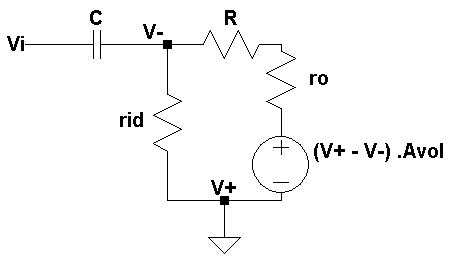
\includegraphics[scale=0.55]{Recursos/Derivador/Circuito_derivador_modelo.png} &
	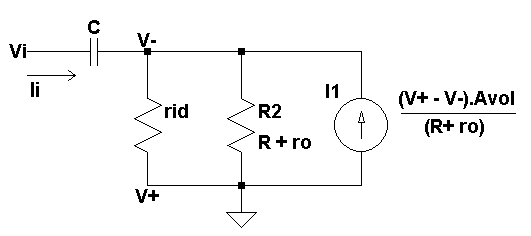
\includegraphics[scale=0.55]{Recursos/Derivador/Circuito_derivador_simplificacion.png}
\end{tabular}
\caption{Circuito derivador con modelo del amplificador y transformaci\'on}
\label{fig:circuito_derivador_impedancia}
\end{figure}

\begin{equation*}
	Y_r = \frac{1}{r_{id}} + \frac{1 + A_{vol}}{R + Z_o} \Rightarrow
	Z_r = \frac{r_{id} \cdot(R + Z_o)}{R + Z_o + r_{id} \cdot(1 + A_{vol})}
\end{equation*}

\begin{equation}
	Z_{in} = \frac{1}{sC} + Z_r
	= \frac{1 + s \cdot \frac{C \cdot r_{id} \cdot (R + Z_o)}{R + Z_o + r_{id} \cdot (1 + A_{vol})}}{s \cdot C}
	\Rightarrow
	Z_{in} = \frac{1 + \frac{s}{2 \pi \cdot 157,98MHz}}{\frac{s}{2 \pi \cdot 7,957MHz}}
	\label{eq:derivador_impedancia_avol_finito}
\end{equation}

En primera instancia, se observa que la impedancia de entrada del circuito derivador no es invariante frente a la frecuencia,
sino que var\'ia, y particularmente para el rango de frecuencias donde $f < 15,79MHz$ la impedancia del mismo, dentro del contexto del an\'alisis, se puede
aproximar a la del capacitor.

\paragraph*{Impedancia de entrada con polo dominante} ahora se adaptan los c\'alculos previos para incluir la apreciaci\'on del polo dominante dentro del an\'alisis de la impedancia de entrada. Operando con la expresi\'on del polo dominante \ref{eq:polo_dominante} se llega a que:

\begin{equation*}
	Z_{in} = \frac{R + Z_o + r_{id} \cdot (A_o + 1 + \frac{s}{\omega_p}) + s \cdot C \cdot r_{id} \cdot (R + Z_o) \cdot (1 + \frac{s}{\omega_p})}{s \cdot C \cdot \left[ (R + Z_o) \cdot (1 + \frac{s}{\omega_p}) + r_{id} \cdot (1 + A_o + \frac{s}{\omega_p}) \right]}
\end{equation*}

\begin{equation*}
	Z_{in} = \frac{1}{s \cdot C} \cdot 
	\frac{1 + s \cdot \frac{R + Z_o + r_{id} + r_{id} \cdot C \cdot \omega_p \cdot(R + Z_o)}{\omega_p \cdot \left[ R + Z_o + r_{id} \cdot (A_o + 1) \right]} + s^{2} \cdot \frac{r_{id} \cdot C \cdot (R + Z_o)}{\omega_p \cdot \left[ R + Z_o + r_{id} \cdot (A_o + 1) \right]}}{1 + s \cdot \frac{R + Z_o + r_{id}}{\omega_p \cdot \left[ R + Z_o + r_{id} \cdot (1 + A_o)\right]}}
\end{equation*}

\begin{align}
	Z_{in} & = \frac{1}{\frac{s}{2 \pi \cdot 7,957MHz}} \cdot
	\frac{1 + s \cdot 11,923 \cdot 10^{-9} + \left(\frac{s}{2 \pi \cdot 153,94kHz}\right)^{2}}{1 + \frac{s}{2 \pi \cdot 14,58MHz}}
	\label{eq:derivador_impedancia_polo_dominante}
\end{align}

Como se puede observar, la impedancia de entrada posee dos ceros complejos y conjugados, ubicados en la frecuencia de corte con $f_o = 153,94kHz$, lo cual establece otra consideración a tener en cuenta con respecto a las limitaciones del circuito, puesto que para esta frecuencia la impedancia de entrada se hace muy chica, produciendose un incremento en el consumo de corriente. Por otro lado, al bajar tanto la impedancia se produce una desadaptaci\'on, es decir, al ser la impedancia de entrada tan peque\~na para esta frecuencia, hay una gran p\'erdida de tensi\'on sobre la resistencia propia de la fuente de la se\~nal.

\paragraph*{Conclusi\'on del an\'alisis} teniendo en cuenta las expresiones finales para caracterizar al circuito derivador con 
la menor idealidad posible, es decir, las ecuaciones \ref{eq:derivador_transfer_polo_dominante} y 
\ref{eq:derivador_impedancia_polo_dominante} se ve como resultado de este an\'alisis que por la forma de la 
funci\'on transferencia el comportamiento derivador se sostiene hasta una frecuencia $f < 154kHz$ aproximadamente, pues hasta esa frecuencia 
se mantiene aproximadamente en $-90^{\circ}$ la fase de la respuesta. No obstante este an\'alisis es estimativo considerando que el valor del $\xi$ es muy cercano a cero puesto
que por no serlo el cambio de fase ocurre antes de dicha frecuencia. Por otro lado, durante este rango de frecuencia la 
 impedancia de entrada est\'a dominada por la del capacitor, con lo cual disminuye hasta que se produce una ca\'ida en el valor 
 de la impedancia y se producen p\'erdidas en la se\~nal que ve el amplificador. Finalmente, el sistema se encuentra subamortiguado, por tanto
 deber\'a poder percibirse tal comportamiento en la respuesta transitoria o en frecuencia del circuito.

\subsubsection{Resultados}
En base a la conclusi\'on del an\'alisis te\'orico realizado, se realizan una serie de simulaciones y mediciones sobre el circuito
para obtener una caracterizaci\'on del mismo y contrastar tales resultados contra lo descripto por lo te\'orico. Vale aclarar que las simulaciones
son graficadas utilizando Monte Carlo para considerar un rango de posibles desviaciones ante la imprecisi\'on de los valores de componentes.

\paragraph*{Respuesta en frecuencia} en las figuras \ref{fig:derivador_bode_modulo} y \ref{fig:derivador_bode_fase} se puede observar
que para el rango de frecuencias donde $f < 100kHz$ aproximadamente, el m\'odulo de la respuesta en frecuencia constrasta con poco error entre
la simulaci\'on, lo te\'orico y la medici\'on. Vale aclarar, que al estar muy subamortiguado el sistema, el cambio de fase se hace muy repentino en torno
a la frecuencia de corte asociada a los polos complejos y conjugados, esto provoca que el comportamiento derivador llegue a operar hasta una alta frecuencia.

Por otro lado, se puede observar que el sobrepico cercano a la frecuencia de corte obtenido te\'oricamente est\'a dentro de los m\'argenes de las aproximaciones
de la simulaci\'on en LTSpice, no obstante, en las mediciones se produce una gran diferencia entre estos valores. Esto \'ultimo se debe a que por un lado la compensaci\'on de un derivador
, como se ver\'a posteriormente, consiste en colocar una resistencia en serie al capacitor y tiene como efecto, entre otros, reducir el subamortiguamiento del sistema. Poniendo a prueba esto \'ultimo,
y considerando que adem\'as de las resistencias par\'asitas por cables y capacitor, aparece la del generador, luego se contrasta contra la simulaci\'on y se ve que ajusta aproximadamente bien. Dicha correcci\'on en
la resistencia en serie del generador para la simulaci\'on corresponde a la figura con el trazo "Simulado R".
Si bien agregando la resistencia del generador justifica la ca\'ida del sobrepico en las mediciones, el valor con el cual se logra ajustar la curva es tomando $R = 25 \Omega $ en serie
 al generador, esto \'ultimo no es muy coherente si se tiene en cuenta que los generadores tienen una impedancia de salida de $R_{g} = 50 \Omega $. Es por esto mismo que se decidi\'o tomar mas mediciones en torno al
 sobrepico con el objetivo de localizarlo con menos error. No obstante, en el proceso de tales mediciones aparecieron algunos inconvenientes que imped\'ian medir correctamente el sobrepico, y se atribuye a tales factores
 el hecho de que el sobrepico obtenido no es realmente el que se produce, sino que el verdadero tiene una magnitud y una frecuencia mayor. Las bases te\'oricas de tal afirmaci\'on salen directo de las conclusiones del an\'alisis
 te\'orico realizado anteriormente, o bien mismo de las mediciones de impedancia de entrada. As\'i, se puede observar que para las frecuencias donde se produce el sobrepico de la transferencia, tambi\'en se produce una ca\'ida abrupta
 en la impedancia de entrada del circuito, y en consecuencia la tensi\'on que ve a la entrada el circuito tambi\'en decrece abruptamente deformandose como se puede observar en la figura \ref{fig:justificacion_derivador}. Se midi\'o las 
 sen\~nales amarilla y verde, es decir, la entrada y salida respectivamente, y se observa que para una entrada que deber\'a de corresponderse con una senoidal, la atenuaci\'on producto de una muy baja impedancia de entrada del orden de $R = 6 \Omega$ 
 no s\'olo produce la saturaci\'on de la salida sino que pierde la forma que esencialmente ten\'ia.
 
 Finalmente, a partir de los $f = 200kHz$ se desv\'ian las curvas te\'orica, medici\'on y simulaci\'on. Esto se atribuye al hecho de que para el orden de estas frecuencias,
 la ganancia produce una saturaci\'on con muy bajas tensiones de salida, sumado a que con altas frecuencias el slew rate limita el rango de operaci\'on. Por lo tanto no se consideran
 apreciables los resultado de mediciones posteriores a $1MHz$ y se puede observar con las desviaciones ya presentadas antes de tal frecuencia.

\begin{figure}[H]
	\centering
	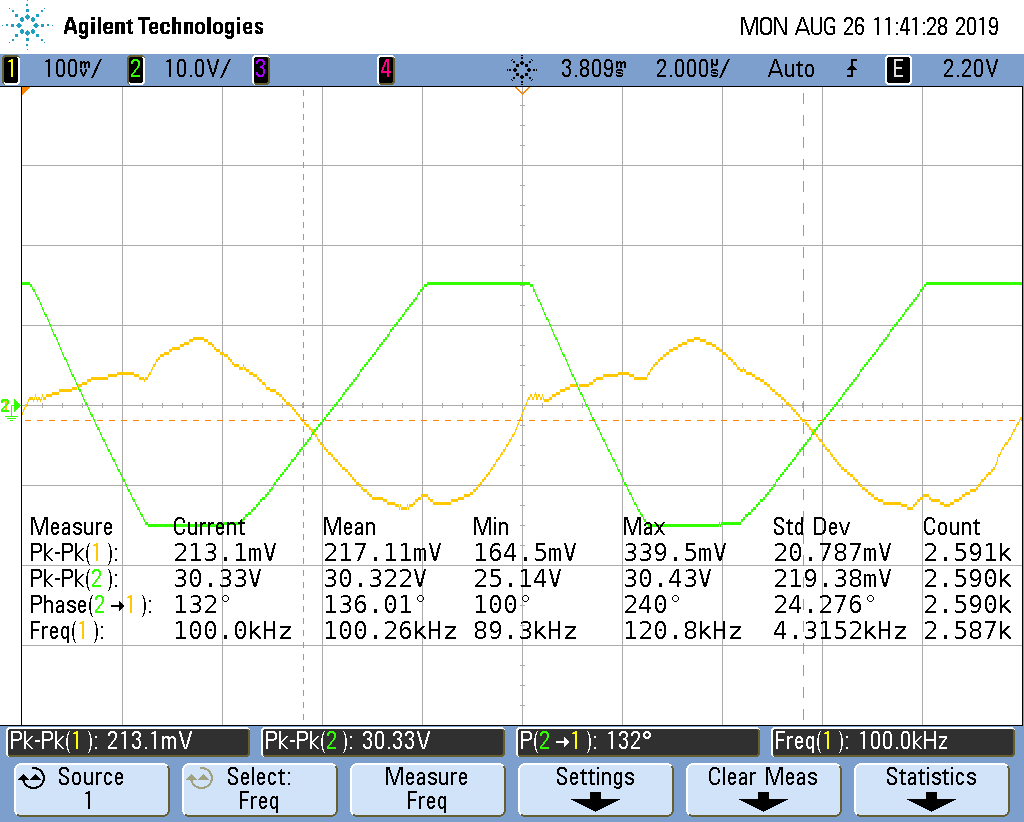
\includegraphics[scale=0.4]{Derivador/Mediciones/Osciloscopio/Justificacion/scope_4.png}
<<<<<<< HEAD
	\caption{Se\~nal amarilla es una entrada senoidal, se\~nal verde es la salida.}
=======
	\caption{Señal amarilla es una entrada senoidal, señal verde es la salida.}
>>>>>>> 1c903573e405a1b067e44751a5fd15495a8566b3
	\label{fig:justificacion_derivador}
\end{figure}

\begin{figure}[H]
	\centering
<<<<<<< HEAD
	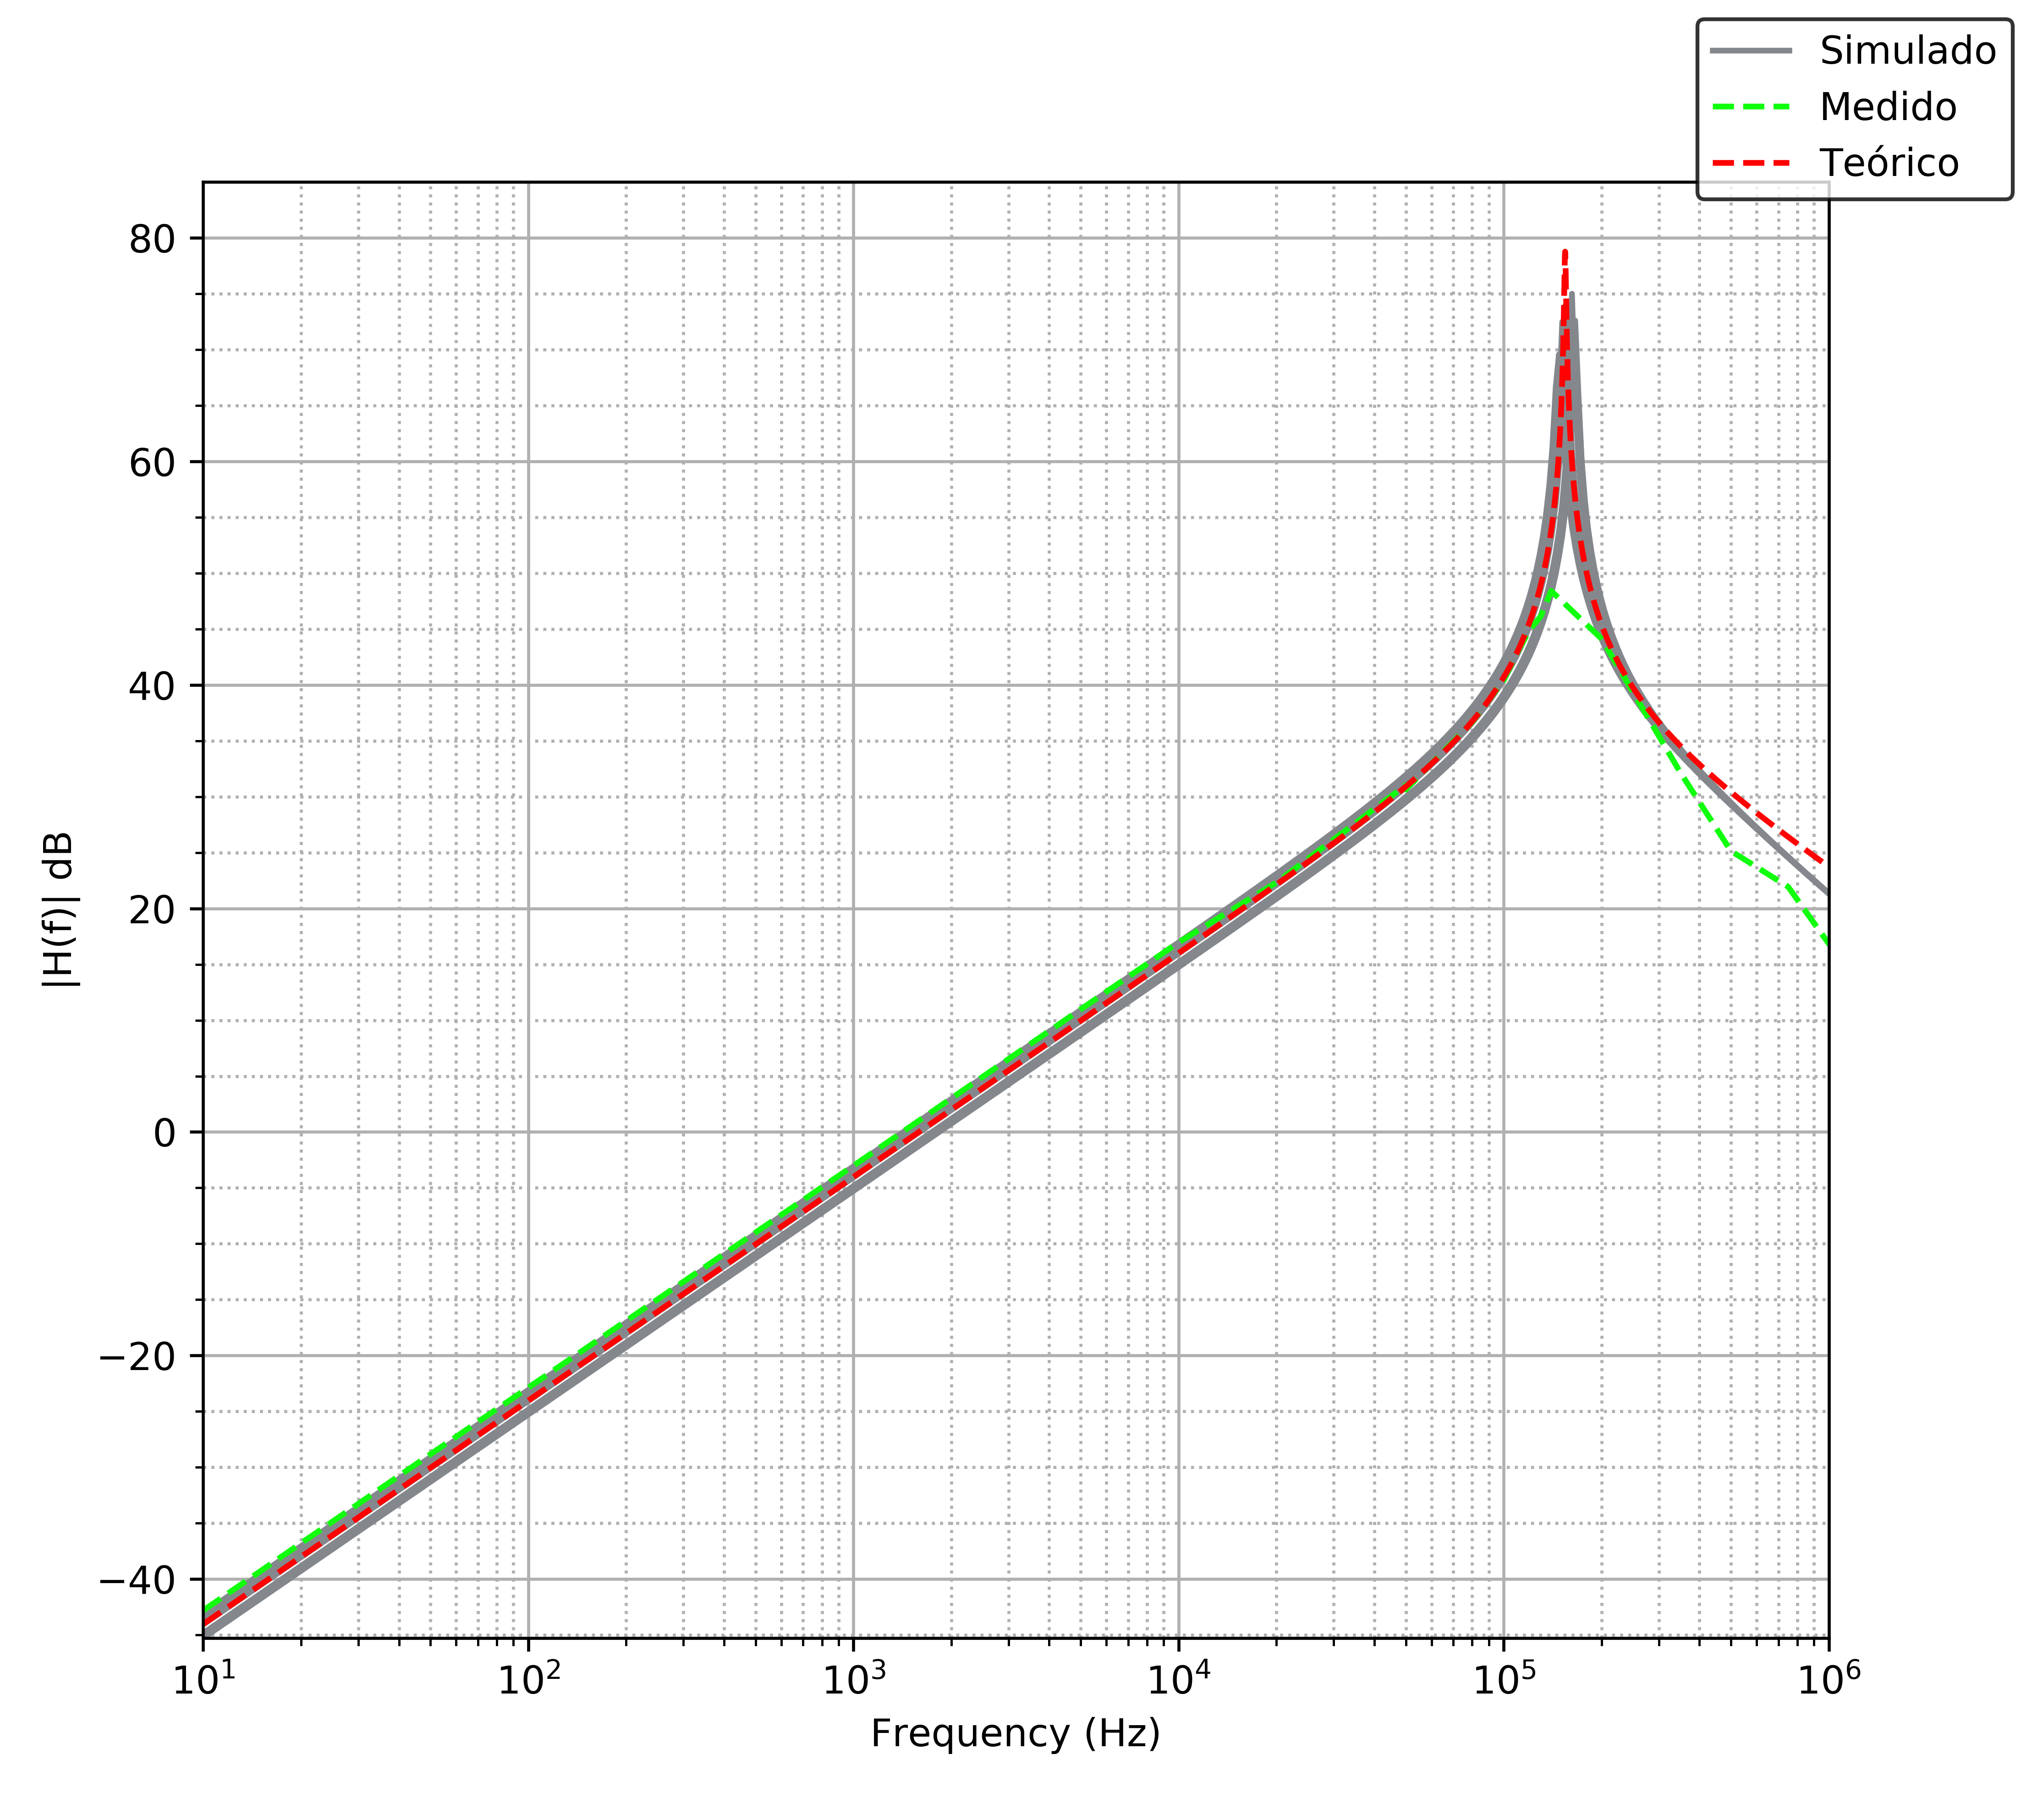
\includegraphics[scale=0.6]{Recursos/Derivador/bode_modulo.png}
=======
	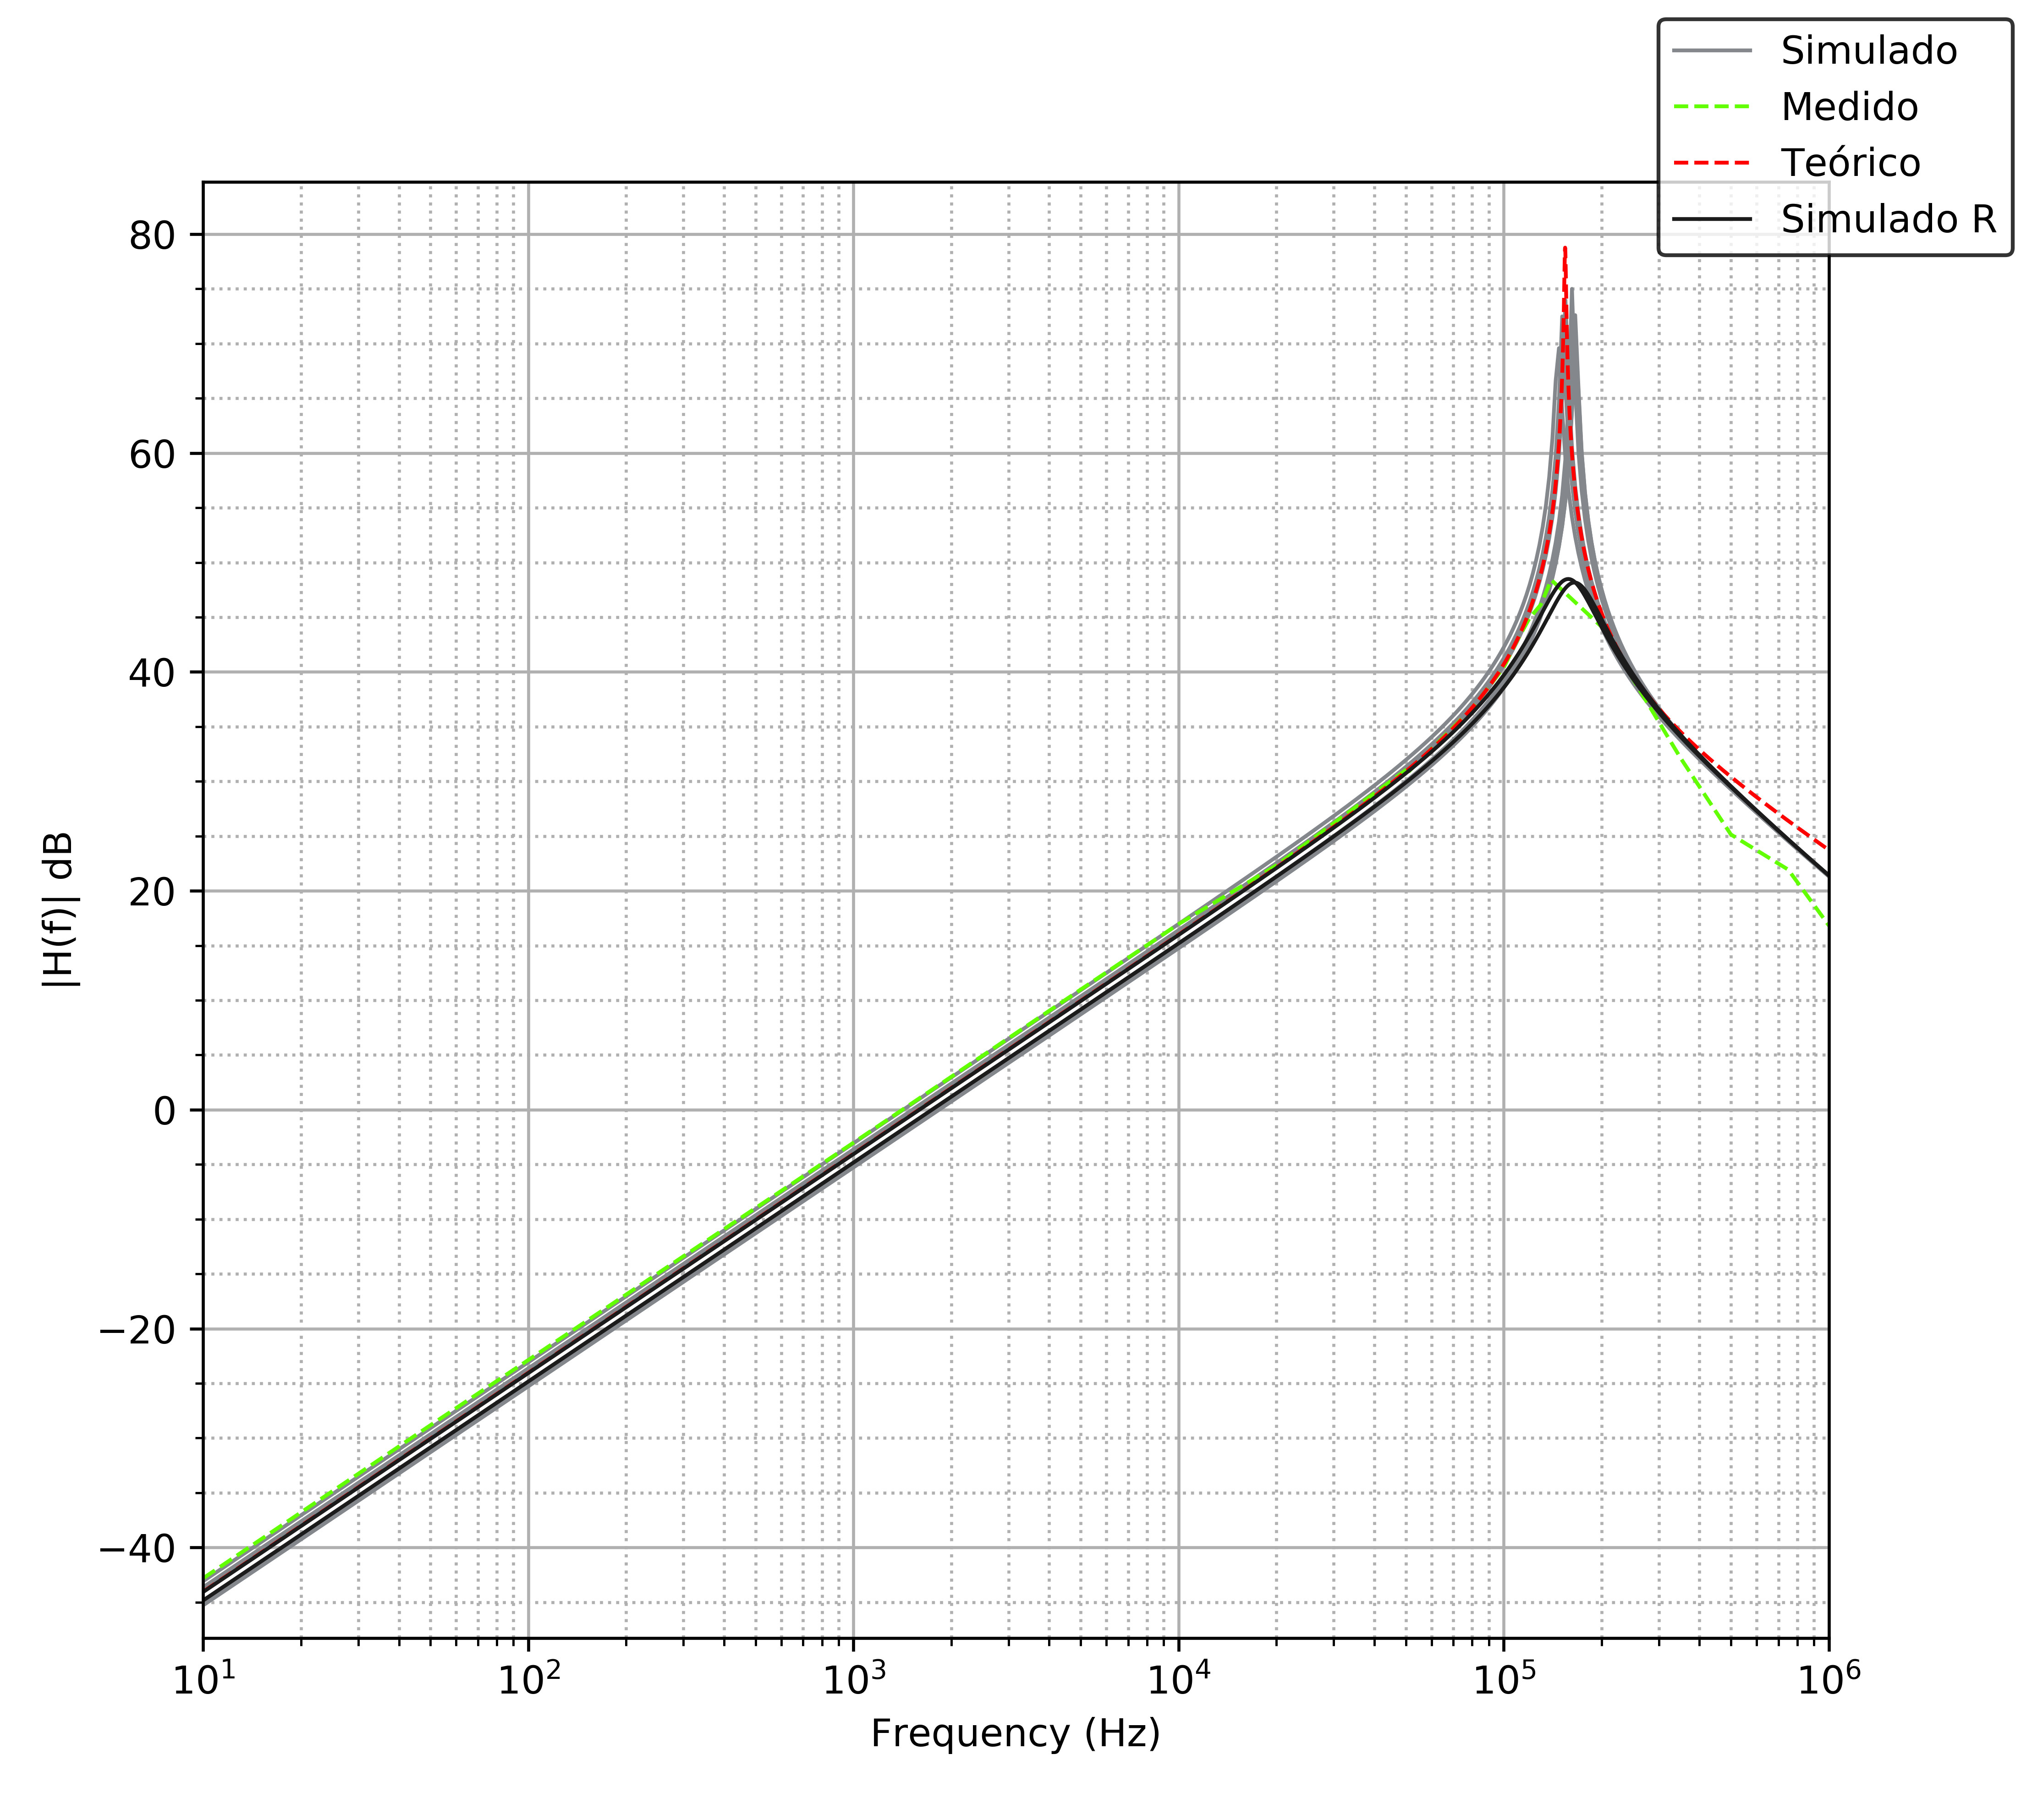
\includegraphics[scale=0.6]{Recursos/Derivador/bode_modulo_correcion.png}
>>>>>>> 1c903573e405a1b067e44751a5fd15495a8566b3
	\caption{Diagrama de bode en m\'odulo de H(f) del derivador}
	\label{fig:derivador_bode_modulo}
\end{figure}

\begin{figure}[H]
	\centering
	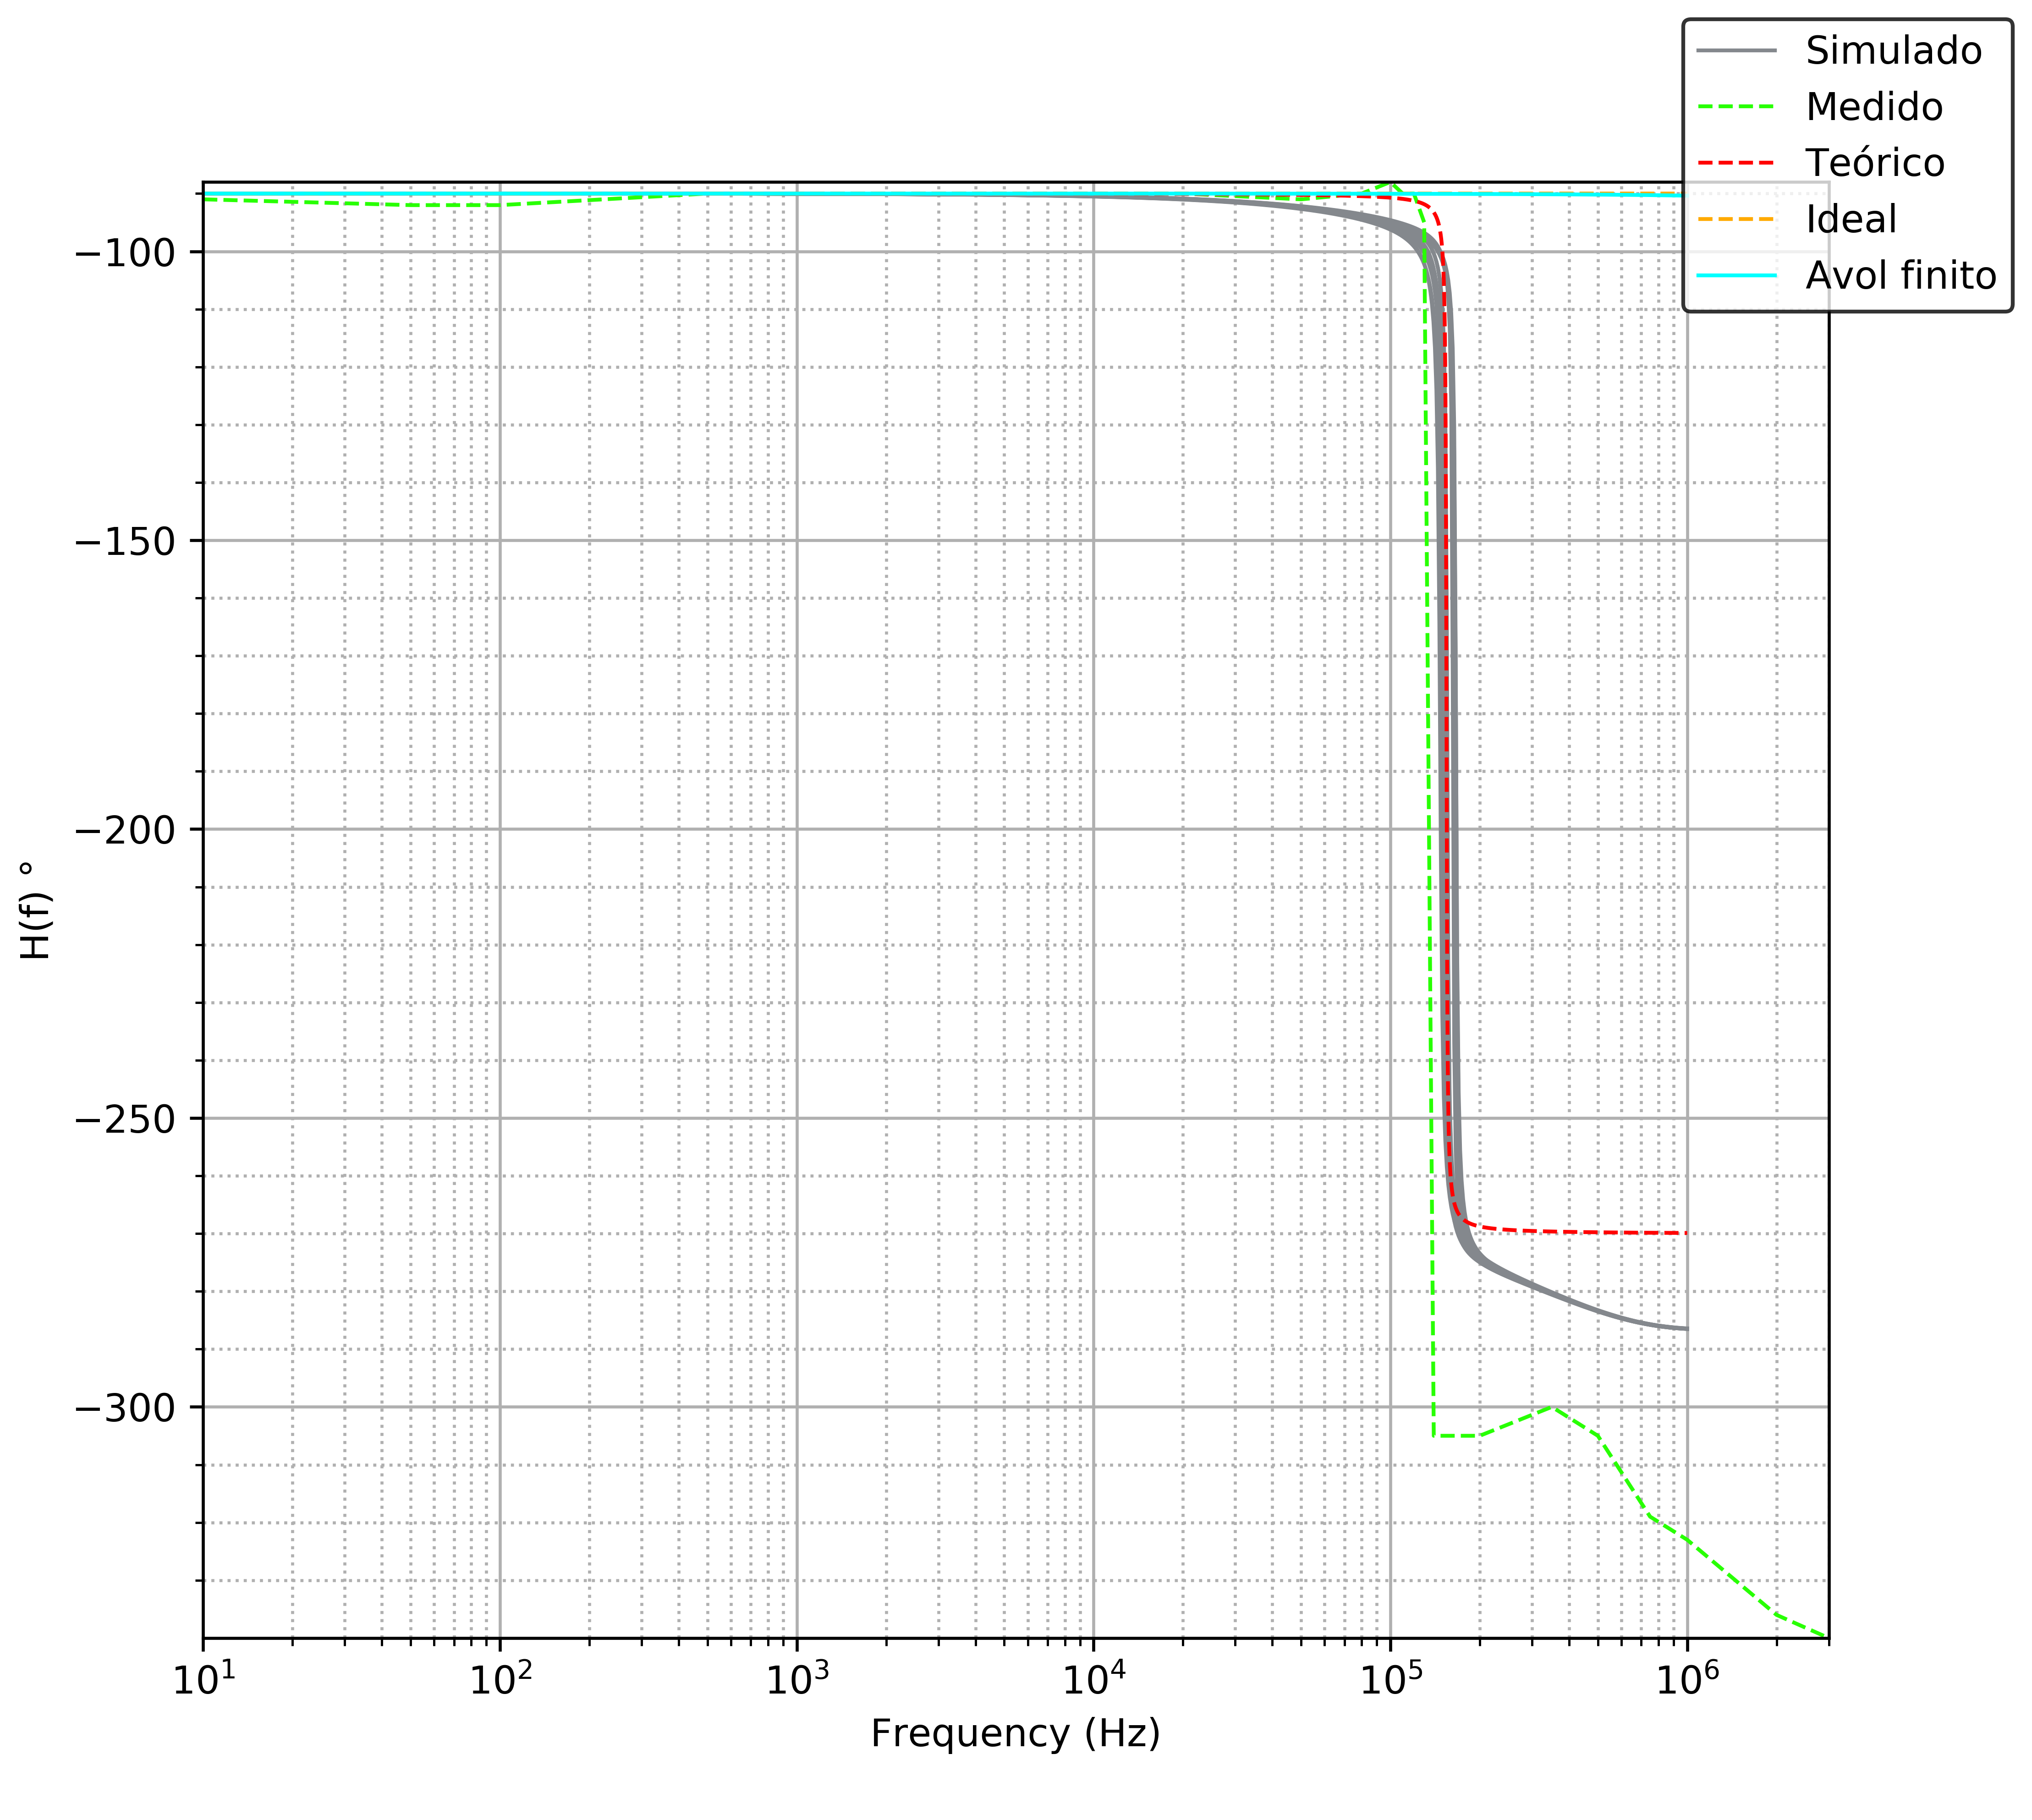
\includegraphics[scale=0.6]{Recursos/Derivador/bode_fase.png}
	\caption{Diagrama de bode en fase de H(f) del derivador}
	\label{fig:derivador_bode_fase}
\end{figure}

\paragraph*{Impedancia de entrada} De los gr\'aficos obtenidos para la medici\'on, simulaci\'on y an\'alisis de la impedancia
de entrada del circuito, se pueden analizar los mismos efectos que para el caso de la respuesta en frecuencia. Esto \'ultimo quiere decir que para frecuencias
menores que $f < 100kHz$ hay poco error entre los resultados obtenidos, mientras que para las dem\'as frecuencias hay desviaciones m\'as apreciables, y se atribuye
al igual que antes al hecho de que para dichas frecuencias la impedancia de entrada produce una gran atenuaci\'on y la ganancia produce saturaci\'on de la salida
con poca tensi\'on, con lo cual no hay forma de obtener para alguna se\~nal de entrada, una salida apreciable, ya que si la tensi\'on pico a pico fuera peque\~na para que no sature,
luego la atenuaci\'on en la entrada por el divisor de tensi\'on entre carga y generador provocar\'ia que no llegue una se\~nal de magnitudes apreciables. Adem\'as llegado el caso
donde estos aspectos no afecten, se ver\'ia que para tales frecuencias el slew rate limitar\'ia la pendiente de crecimiento.

\begin{figure}[H]
	\centering
	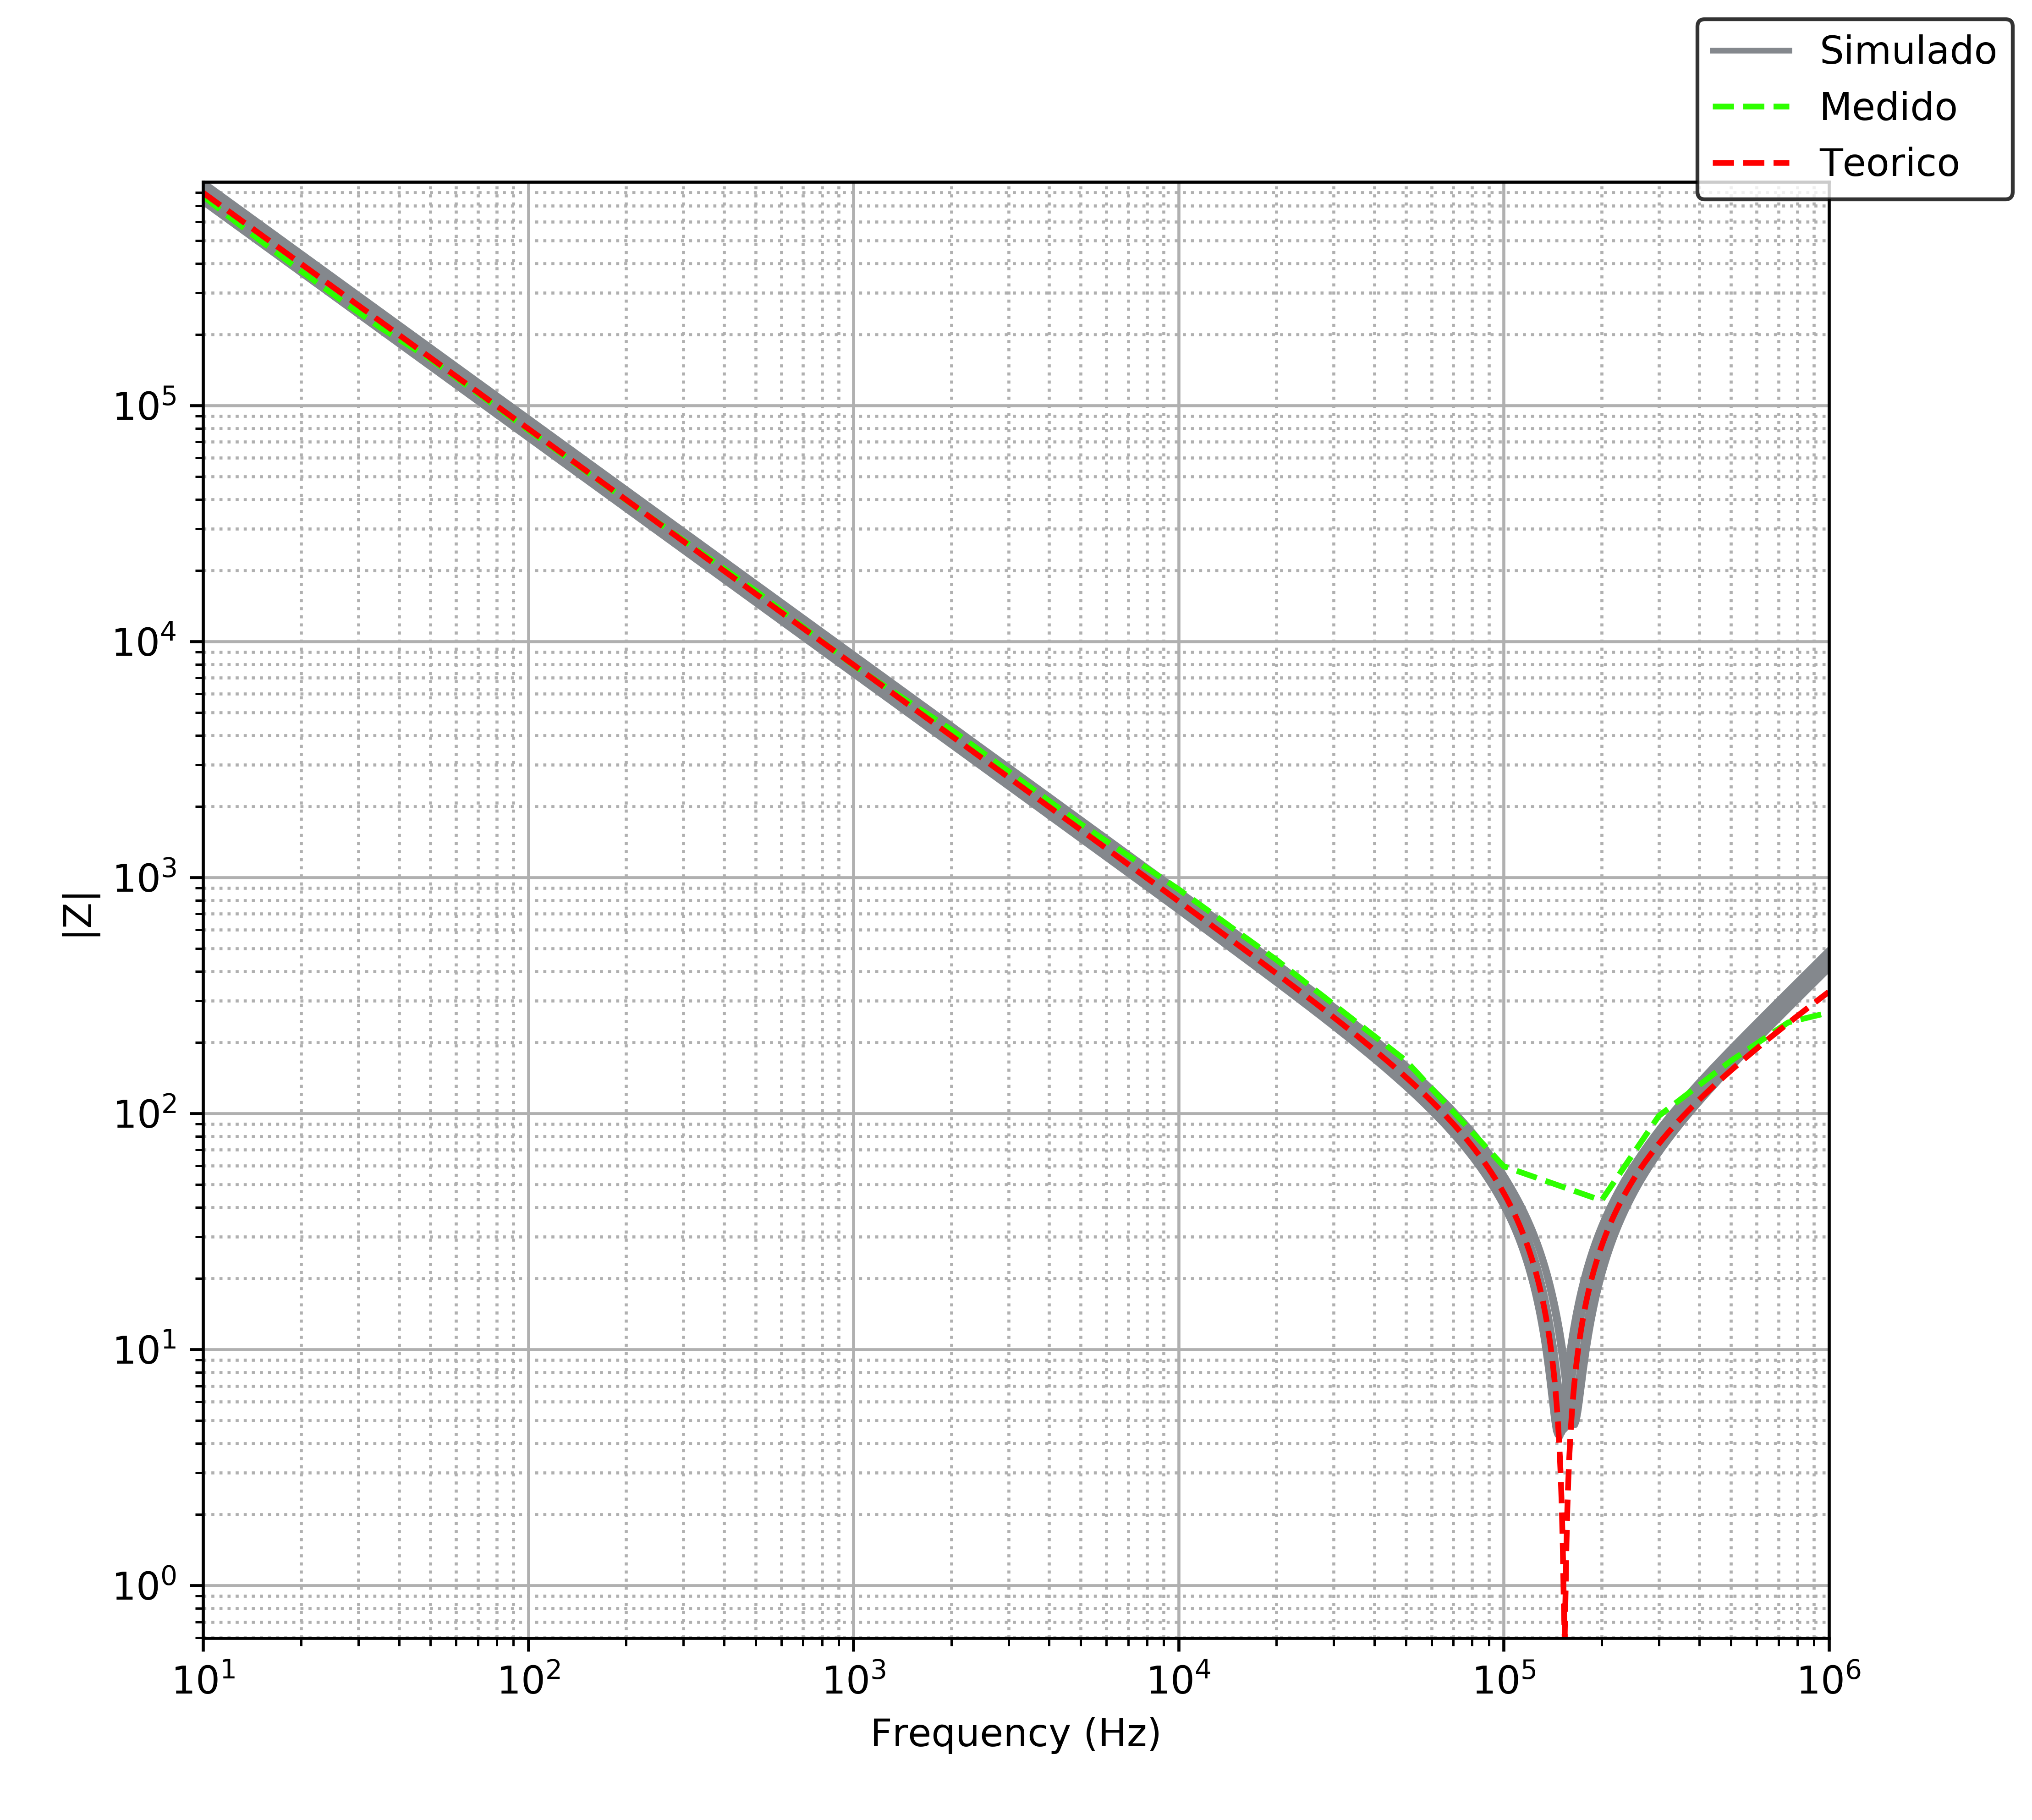
\includegraphics[scale=0.7]{Recursos/Derivador/impedancia_modulo.png}
	\caption{Impedancia de entrada en m\'odulo, graficada con escalas logar\'itmicas}
	\label{fig:derivador_impedancia_modulo}
\end{figure}

\begin{figure}[H]
	\centering
	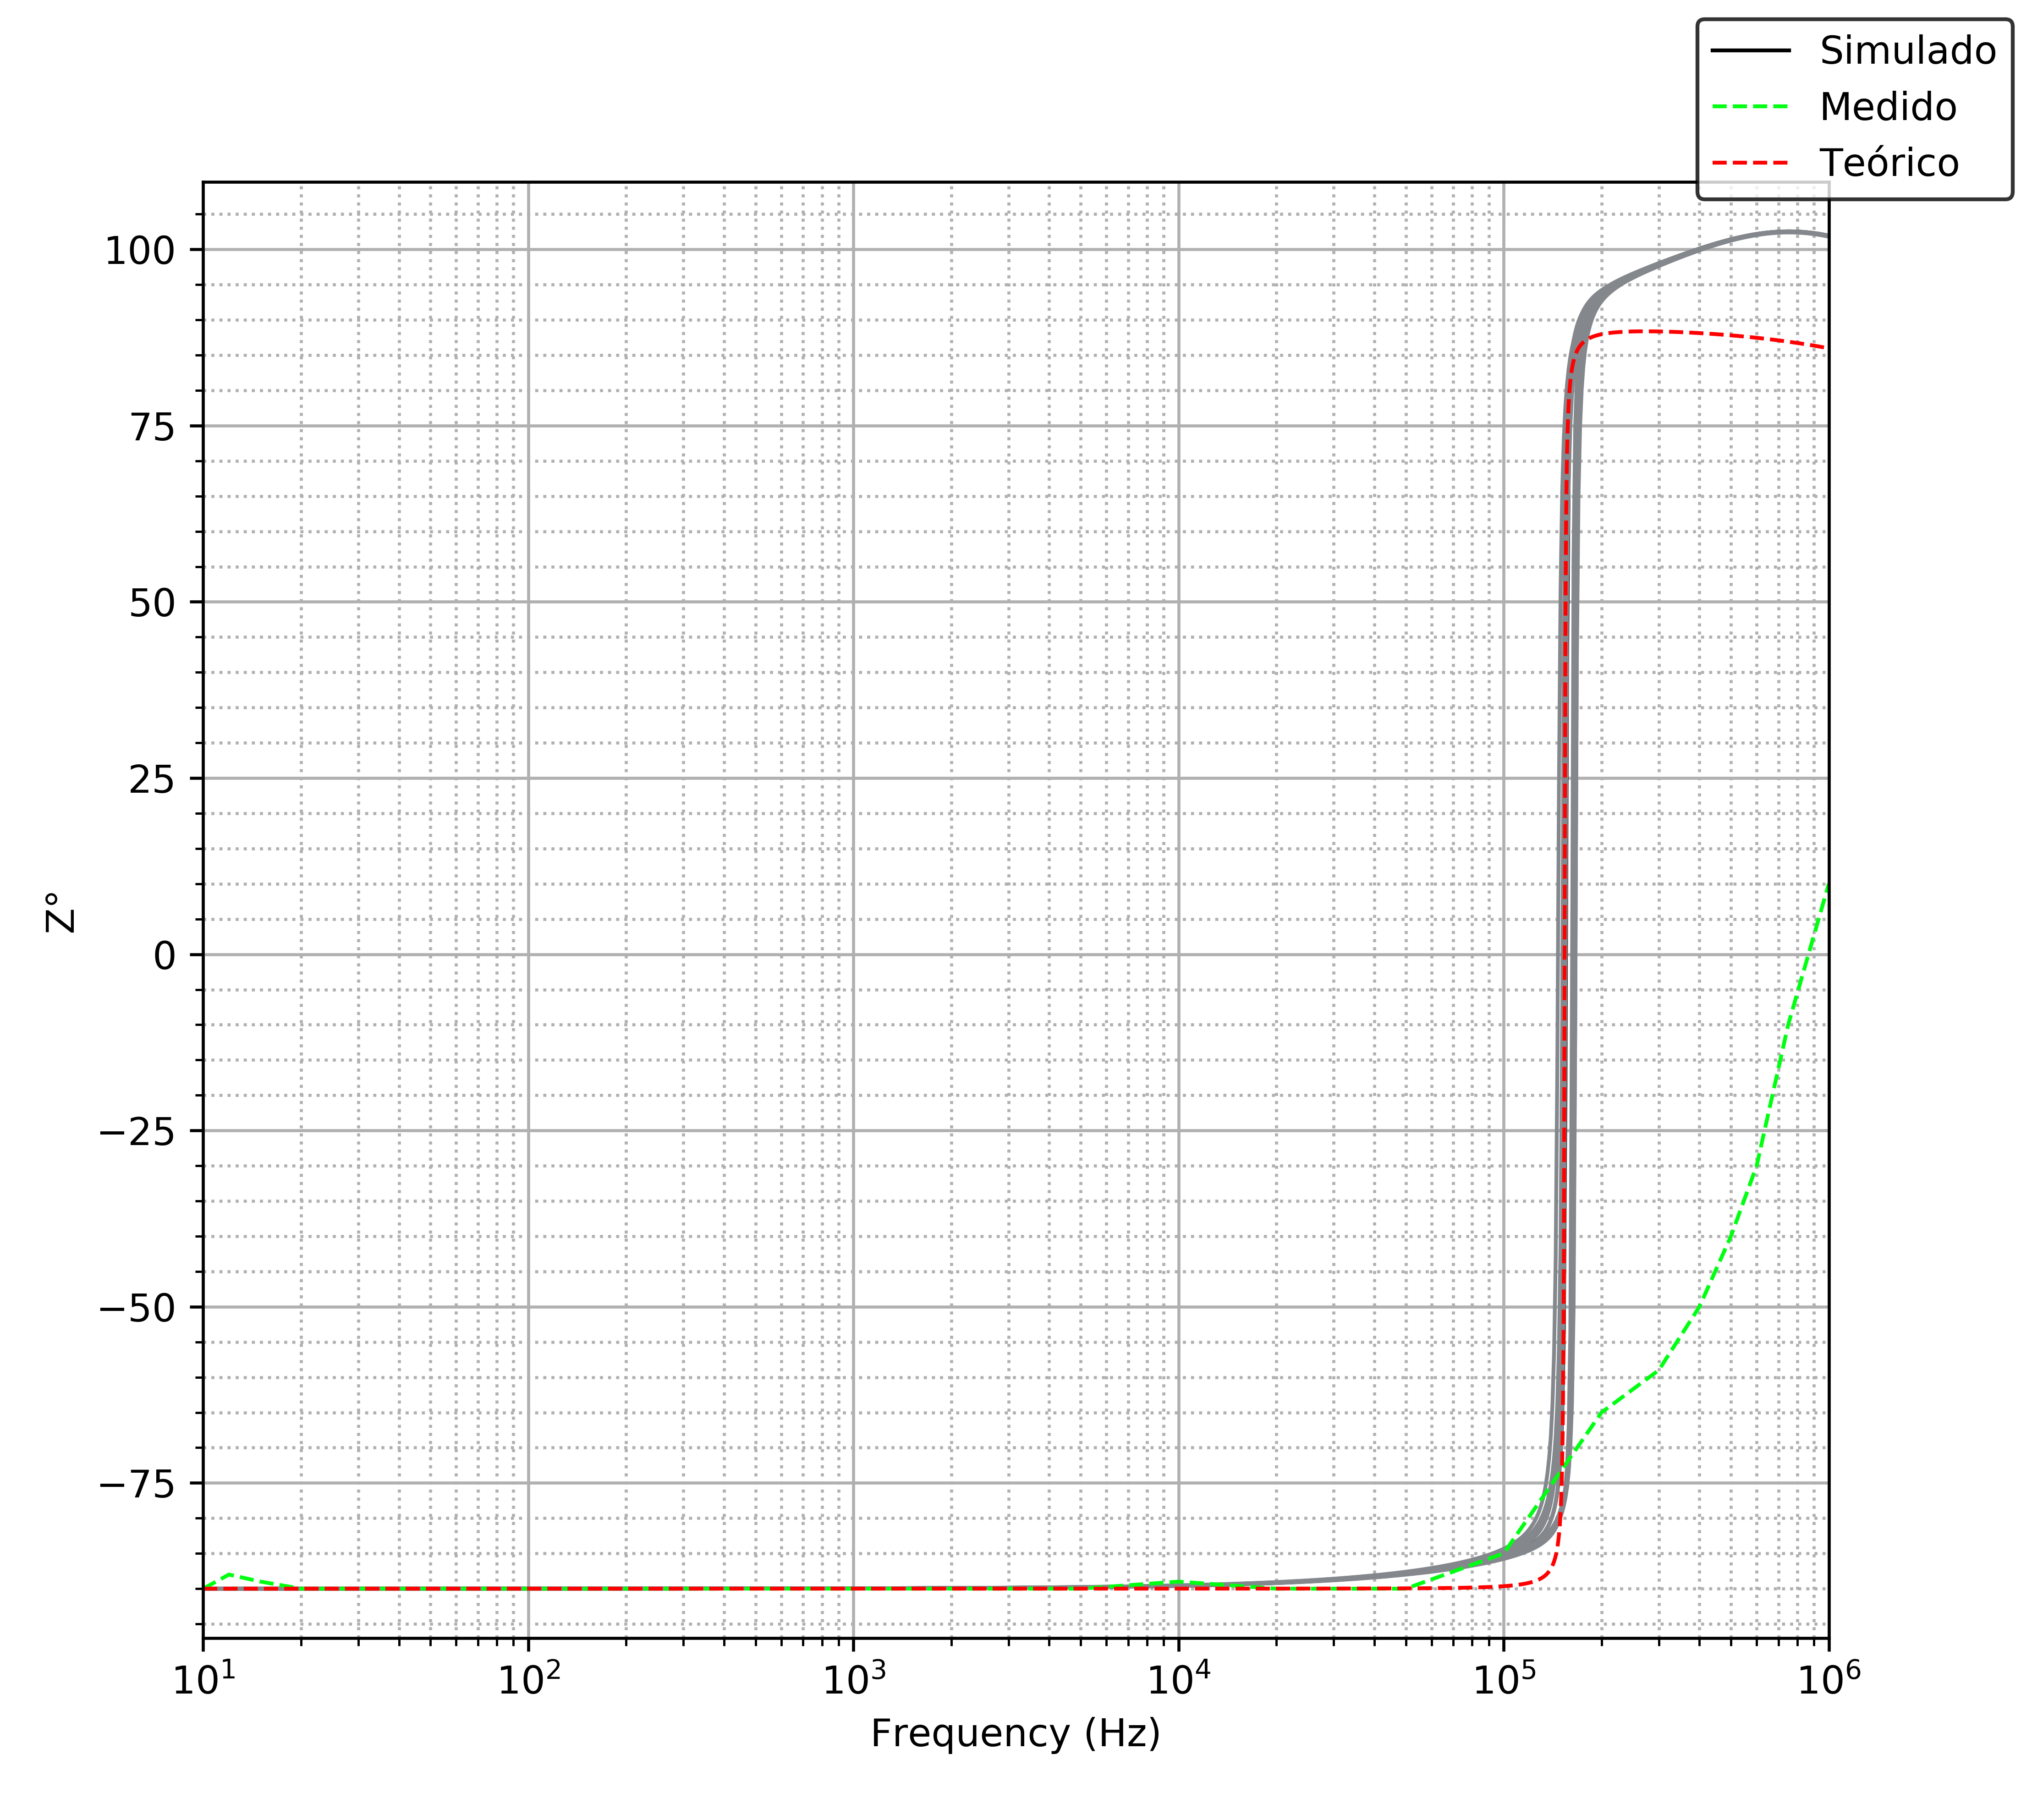
\includegraphics[scale=0.7]{Recursos/Derivador/impedancia_fase.png}
	\caption{Impedancia de entrada en fase, graficada con escalas logar\'itmicas}
	\label{fig:derivador_impedancia_fase}
\end{figure}

<<<<<<< HEAD
\paragraph*{Respuesta a se\~nales no senoidales} en la figura \ref{fig:derivador_respuestas} se pueden observar las respuestas
=======
\paragraph*{Respuesta a señales no senoidales} en la figura \ref{fig:derivador_respuestas} se pueden observar las respuestas
>>>>>>> 1c903573e405a1b067e44751a5fd15495a8566b3
al derivador sin compensar para cuatro casos diferentes, una triangular con simetr\'ia del $80\%$ y una frecuencia de $10kHz$,
una triangular con simetr\'ia de $50\%$ y frecuencia de $1kHz$, una cuadrada de frecuencia $1kHz$ con duty del $50\%$ y finalmente una cuadrada
de frecuencia $10kHz$ y duty del $50\%$.

De estos resultados y otros que pueden observarse cambiando la frecuencia y amplitud de los est\'imulos mencionados, puede observarse que al estar subamortiguado,
el sistema tiene una respuesta transitoria que afecta a la transici\'on de los estados de la salida, y si bien puede apreciarse la operaci\'on de derivar sobre la misma,
la oscilaci\'on amortiguada se presenta como un efecto indeseado cuando lo que se busca en el sistema es puramente el proceso de derivar la entrada. Esto implica que desde otro enfoque distinto,
el temporal, se pueden contrastar otras consecuencias del subamortiguamiento del sistema adem\'as de las obtenidas en el dominio de la frecuencia. Tales consecuencias son las que dan pie a la necesidad
de compensar el circuito de alguna forma, como se ver\'a a continuaci\'on.

\begin{figure}[H]
	\centering
	\begin{tabular}{c c}
		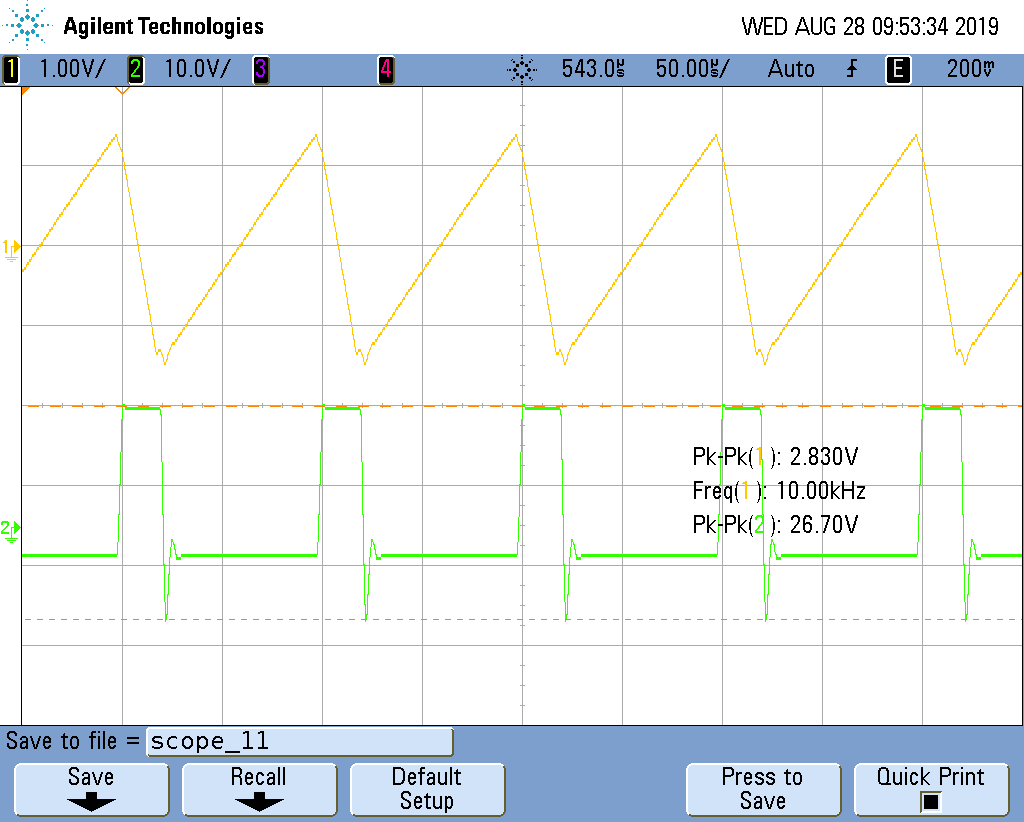
\includegraphics[scale=0.2]{Derivador/Mediciones/Osciloscopio/PCB_Sin_Compensar/scope_11.png} &
		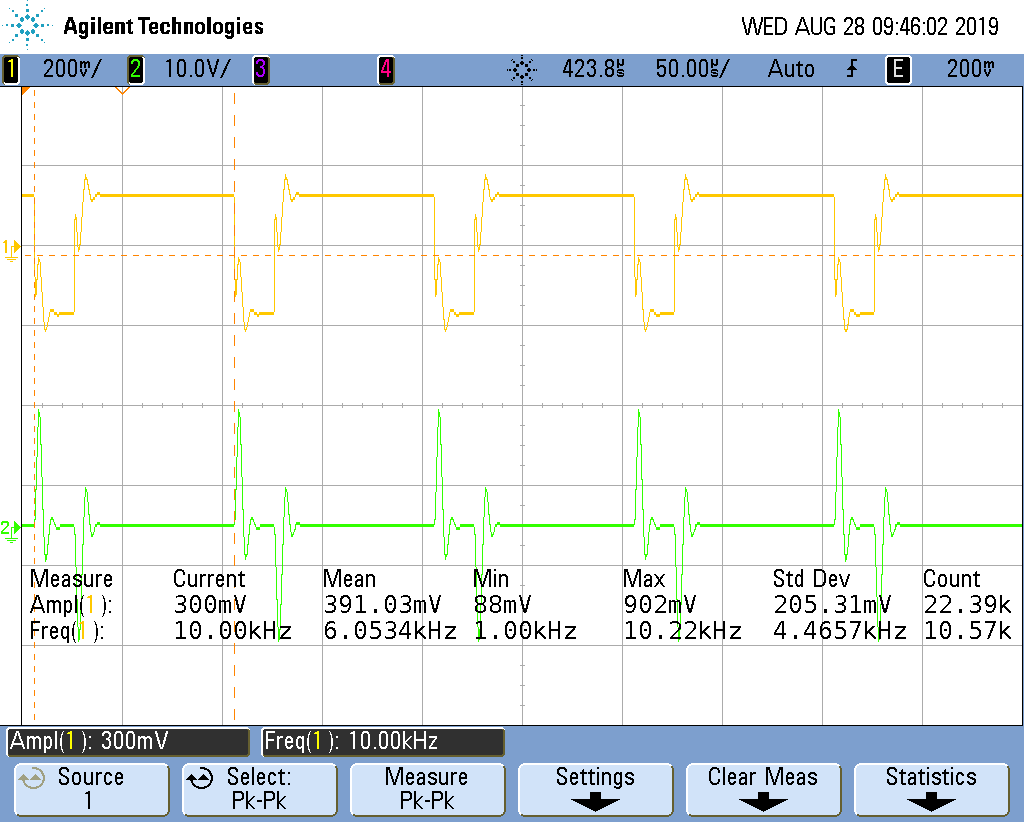
\includegraphics[scale=0.2]{Derivador/Mediciones/Osciloscopio/PCB_Sin_Compensar/scope_3.png} \\
		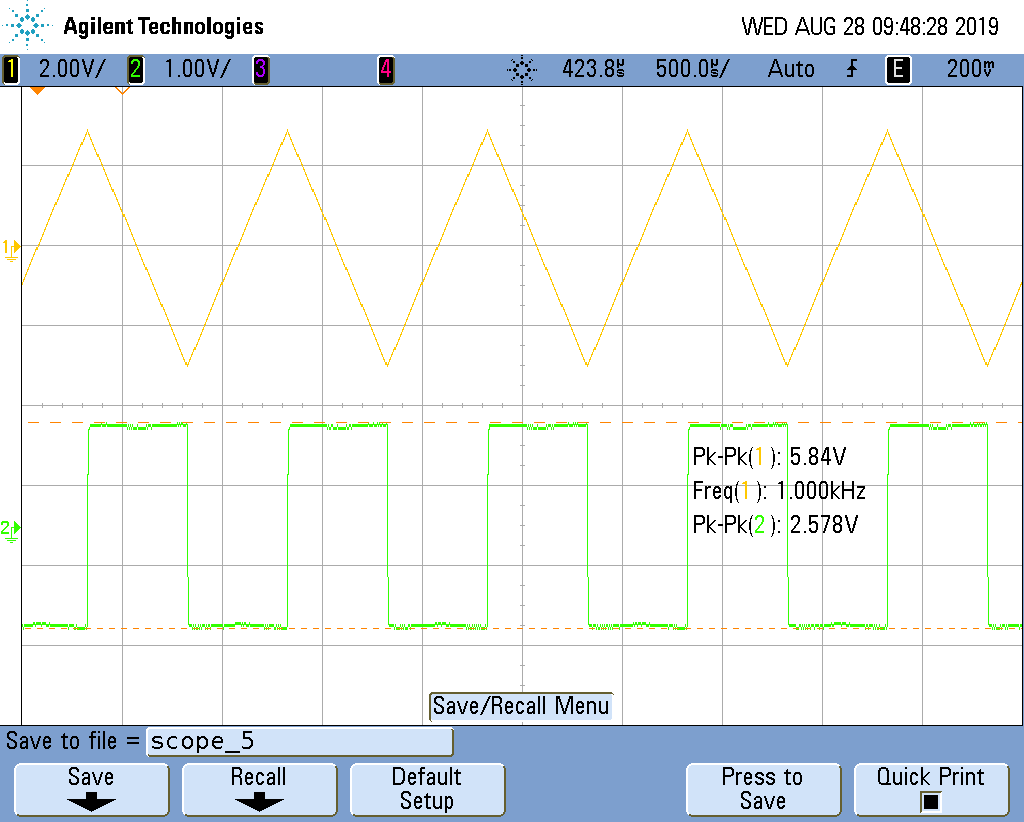
\includegraphics[scale=0.2]{Derivador/Mediciones/Osciloscopio/PCB_Sin_Compensar/scope_5.png} &
		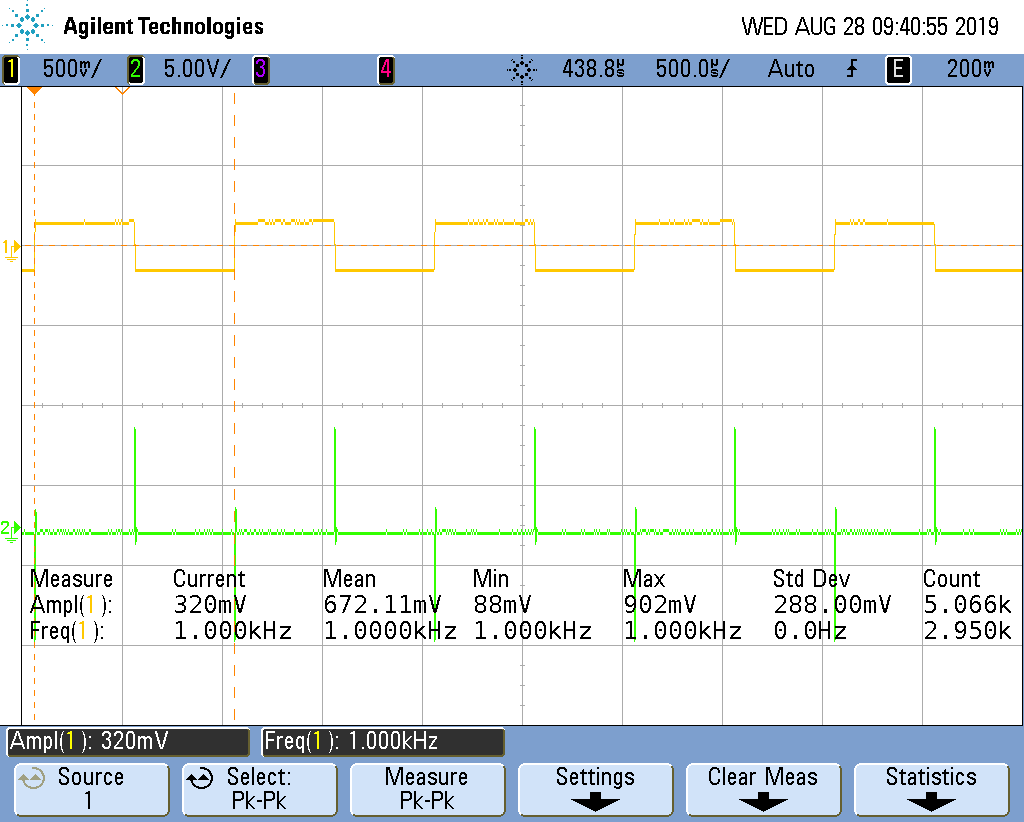
\includegraphics[scale=0.2]{Derivador/Mediciones/Osciloscopio/PCB_Sin_Compensar/scope_7.png}
	\end{tabular}
<<<<<<< HEAD
	\caption{Entrada y salida, se\~nal amarilla y verde respectivamente.}
=======
	\caption{Entrada y salida, señal amarilla y verde respectivamente.}
>>>>>>> 1c903573e405a1b067e44751a5fd15495a8566b3
	\label{fig:derivador_respuestas}
\end{figure}

	\subsection{Circuito derivador compensado}
En la secci\'on anterior se analiz\'o el circuito derivador sin compensaci\'on y se lleg\'o a la conclusi\'on de que, como tal,
si bien ten\'ia un amplio rango de frecuencias en las cuales su comportamiento era la de un derivador, se encontraba en un estado de subamortiguamiento
tanto en funci\'on transferencia como en impedancia de entrada que produci\'a efectos indeseados. Por lo tanto, m\'as all\'a del hecho de que por ser subamortiguado con un bajo
valor de $\xi$ provoca que la transici\'on de fase se haga m\'as abrupta y el margen de funcionamiento como derivador sea mayor, la atenuaci\'on de la impedancia de entrada, saturaci\'on de la salida por ganancia
grande para altas frecuencias y los efectos oscilatorios amortiguados en la transici\'on de la respuesta temporal hacen del circuito anterior un opci\'on poco provechosa.
Por tanto, se propone a continuaci\'on una modificaci\'on al circuito con el fin de compensar tales efectos de la forma m\'as efeciente posible.

\subsubsection{An\'alisis Te\'orico}

\begin{figure}[H]
	\centering
	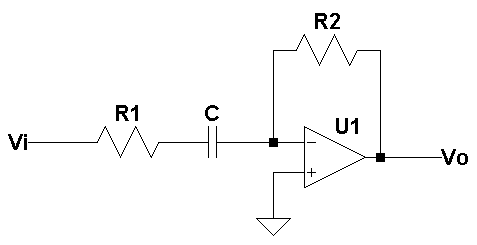
\includegraphics[scale=0.7]{Recursos/Derivador_compensado/Circuito_derivador_compensado.png}
	\caption{Circuito derivador compensado}
	\label{fig:derivador_compensado_circuito}
\end{figure}

En el circuito derivador que se analizar\'a a continuaci\'on se coloca una compensaci\'on 
que consiste en una resistencia en serie en la entrada con el capacitor, esto se debe a que 
se busca compensar los efectos del mismo para altas frecuencias. En altas frecuencias, el 
capacitor tiene una impedancia muy peque\~na con lo cual la ganancia del amplificador 
inversor aumentar\'a y la salida superar\'a la tensi\'on de alimentaci\'on del 
amplificador operacional, produci\'endose as\'i la saturaci\'on del circuito. 
Por otro lado, en cierta parte como la impedancia de entrada depende del capacitor, al 
reducirse tanto a medida que aumenta la frecuencia, disminuye la impedancia de entrada 
y se producen mayores p\'erdidas en la tensi\'on del generador que recibe el circuito.

\paragraph*{Funci\'on transferencia en condiciones ideales} haciendo uso de las condiciones de idealidad que ya se mencionaron para el circuito derivador, a partir de la expresi\'on de la ganancia o transferencia de un amplificador inversor ideal, se llega a que:

\begin{align*}
		H(s) & = \frac{V_o(s)}{V_i(s)} = \frac{-R_2}{R_1 + \frac{1}{s \cdot C}} \\
		& = - \frac{s \cdot C \cdot R_2}{1 + s \cdot C \cdot R_1} \\
\end{align*}

\paragraph*{Funci\'on transferencia con $A_{vol}$ finito} asumiendo que la corriente de entrada del amplificador operacional no es apreciable con respecto a las corrientes de la red L de realimentaci\'on, se plantean las tensiones en las entradas y utilizando la expresi\'on de tensi\'on de salida, se obtiene que:

\begin{equation*}
	v^{-} = V_o \cdot \frac{R_1 + \frac{1}{s \cdot C}}{R_1 + R_2 + \frac{1}{s \cdot C}} + V_i \cdot \frac{R_2}{R_1+ R_2 + \frac{1}{s \cdot C}}
\end{equation*}

\begin{equation*}
	V_o = (v^{+} - v^{-}) \cdot A_{vol} \Rightarrow
	V_o \cdot \left[ 1 + \frac{A_{vol} \cdot (1 + s \cdot C \cdot R_1)}{1 + s \cdot C \cdot (R_1 + R_2)} \right] =
	- V_i \cdot \frac{A_{vol} \cdot (s \cdot C \cdot R_2)}{1 + s \cdot C \cdot (R_1 + R_2)}
\end{equation*}

\begin{equation}
	H(s) = \frac{V_o(s)}{V_i(s)} = - \frac{\frac{s \cdot A_{vol} \cdot C \cdot R_2}{1 + A_{vol}}}{1 + s \cdot \frac{C \cdot (R_2 + R_1 \cdot(1 + A_{vol}))}{1 + A_{vol}}}
	\label{eq:derivador_compensado_finito}
\end{equation}

\paragraph*{Funci\'on transferencia con polo dominante} finalmente si se considera la ecuaci\'on anterior obtenida en \ref{eq:derivador_compensado_finito} y se reemplaza el $A_{vol}$ por la funci\'on que contiene el polo dominante, entonces se llega a que:

\begin{align*}
	H(s) & = \frac{-s \cdot C \cdot R_2 \cdot A_o}{\left( 1 + \frac{s}{\omega_p} \right) \cdot \left( 1 + s \cdot C \cdot (R_1 + 	R_2) \right) + A_o \cdot(1+ s \cdot C \cdot R_1)} \\
	& = - \frac{ \frac{s \cdot c \cdot R_2 \cdot A_o}{A_o + 1} }{1 + s \cdot \frac{1+ \omega_p \cdot \left( A_o \cdot C \cdot R_1 + C \cdot ( R_1 + R_2) \right)}{\omega_p \cdot ( 1 + A_o)} + s^{2} \cdot \frac{C \cdot (R_1 + R_2)}{\omega_p \cdot (1+ A_O)}}
\end{align*}

De esta \'ultima expresi\'on se puede ver del denominador que hay un segundo orden, entonces se procede a obtener sus par\'ametros caracter\'isticos y as\'i determinar su comportamiento.

\begin{equation}
	\omega_o = \sqrt{\frac{\omega_p \cdot ( A_o + 1 ) }{C \cdot ( R_1 + R_2 ) }}
\end{equation}

\begin{equation}
	\xi = \frac{\left[ 1 + \omega_p \cdot C \cdot ( R_1 \cdot (1 + A_o) + R_2) \right] }{2 \cdot \sqrt{\omega_p \cdot C \cdot (A_o + 1) \cdot (R_1 + R_2)}}
	\label{eq:formula_xi}
\end{equation}

Ahora bien, para poder completar el an\'alisis del circuito es necesario determinar el valor de la resistencia $R_1$ la cual no ha sido determinada pues fue agregada a forma de compensaci\'on. Para poder determinar su valor se requieren los siguientes criterios: que no hayan sobrepicos en la funci\'on de transferencia y pueda funcionar hasta la mayor frecuencia posible, adem\'as debe tener un error en la fase menor a 3 grados.

Para poder implementar estas condiciones en el circuito, hay que observar que en la funci\'on transferencia seg\'un sea el caso, primero el denominador debe tener un valor de $\xi \geqslant{1}$ dado que se evita as\'i un sistema subamortiguado cuya respuesta en frecuencia presente un sobrepico. Esta condici\'on se cumple partiendo de la ecuaci\'on \ref{eq:formula_xi}:

\begin{align*}
	& \xi \geqslant{1} \Leftrightarrow \\
	& 1 + \omega_p \cdot C \cdot (R_1 \cdot (A_o + 1) + R_2) \geqslant 2 \cdot \sqrt{\omega_p \cdot C \cdot (A_o + 1) \cdot (R_1 + R_2)} \Leftrightarrow \\
	& R_1^{2} \cdot \alpha + R_1 \cdot \beta + \gamma \geqslant 0
\end{align*}

\begin{align*}
	& \alpha = \omega_p^{2} \cdot C^{2} \cdot (A_o+1)^{2} \\
	& \beta = 2 \cdot \omega_p \cdot C \cdot ( A_o + 1 ) \cdot (R_2 \cdot \omega_p \cdot C - 1) \\
	& \gamma = (1 + \omega_p^{2} \cdot R_2^{2} \cdot C^{2} + \omega_p \cdot C \cdot R_2 \cdot(- 2 - 4 \cdot A_o)
\end{align*}

Resolviendo la cuadr\'atica y encontrando sus ra\'ices, se puede ver que el rango de resistencia con sentido f\'isico para los cuales se logra que el sistema se comporte sobreamortiguado o cr\'iticamente amortiguado, son aquellos donde $R_1 \geqslant 103,48 \Omega$. Por otro lado, para conseguir que el circuito derivador opere hasta la mayor frecuencia posible, habiendo descartado el casos subamortiguado para evitar los sobrepicos en la respuesta en frecuencia, se desea que en el caso \'optimo se encuentre en un amortiguamiento cr\'itico. Esto se debe a que de esta forma en la mayor frecuencia de corte posible se produce la ca\'ida a 40dB/dec, mientras que en un escenario sobreamortiguado el polo se separar\'ia en dos frecuencias de corte reduciendo el ancho de banda disponible.

Con el fin de cumplir con estas condiciones y obtener como resultado el circuito con mejor rendimiento en t\'erminos del ancho de banda donde opera, se coloca un preset en vez de una resistencia fija para poder calibrar el sistema en un valor de aproximadamente $R = 103,487 \Omega$. 

Este proceso de calibraci\'on consiste en utilizar el generador de funciones para excitar al circuito con un escal\'on. Por ser una entrada $V_i(s) = \frac{K}{s}$ con K un valor de amplitud dado, y tener un sistema derivador, la salida debiera de ser una delta de dirac que se ver\'a acotada por la saturaci\'on del amplificador operacional. No obstante, en la transici\'on de la respuesta del circuito se ver\'a la respuesta natural del mismo donde se podr\'a analizar si est\'a en cualquiera de los casos subamortiguado, sobreamortiguado o cr\'iticamente amortiguado, con lo cual se debe mover el preset hasta entrar en la zona sobreamortiguada y luego reducir su valor ligeramente hasta observar que en la salida se tiene el decrecimiento exponencial de menor constante de tiempo sin producir subamortiguamiento.

\begin{figure}[H]
	\centering
	\begin{tabular}{c c}
		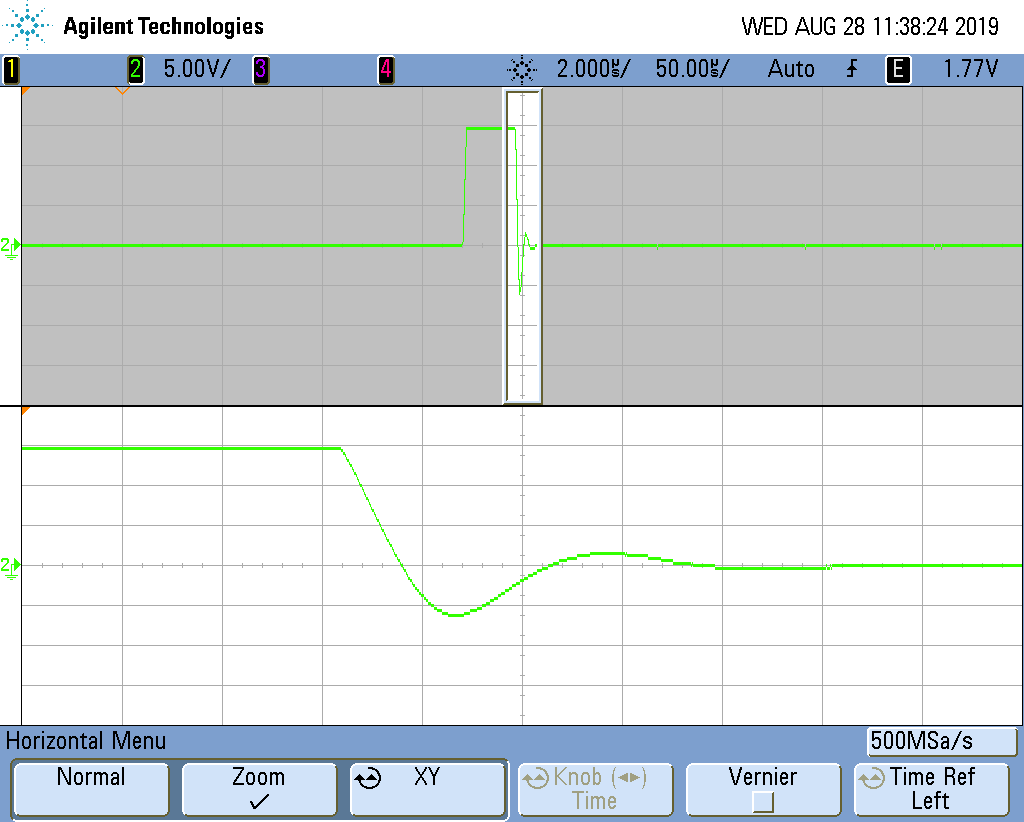
\includegraphics[scale=0.2]{Derivador/Mediciones/Osciloscopio/PCB_Compensado/Calibracion/scope_19.png} &
		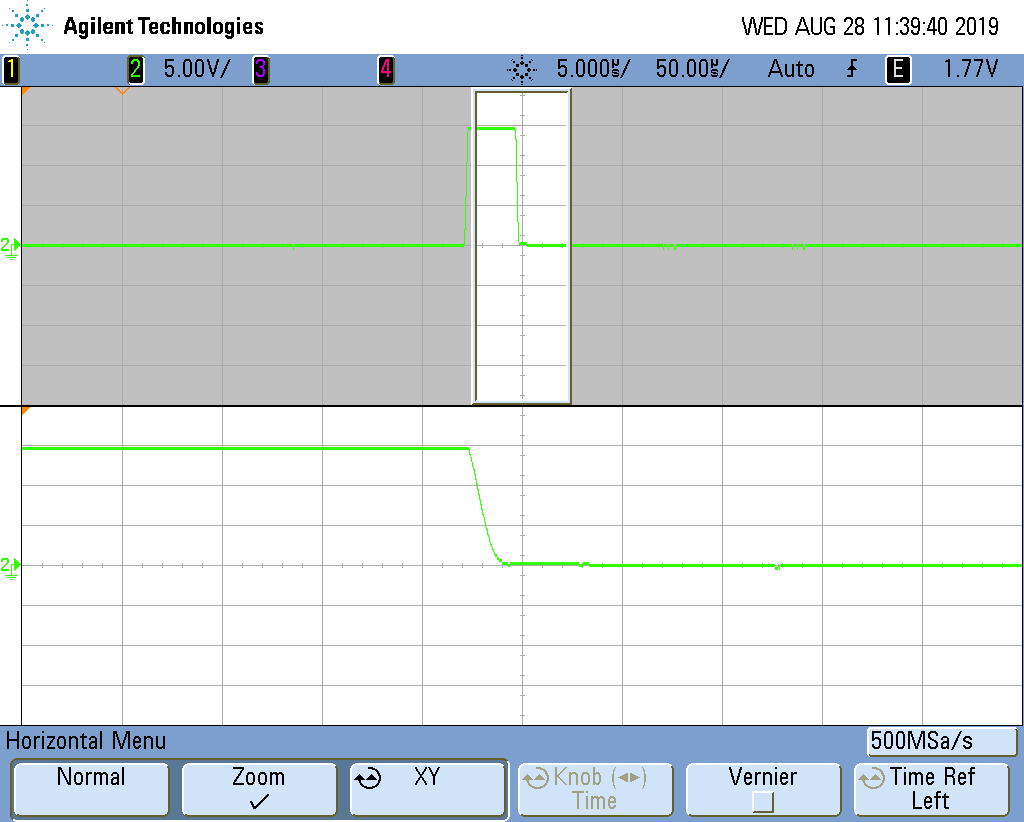
\includegraphics[scale=0.2]{Derivador/Mediciones/Osciloscopio/PCB_Compensado/Calibracion/scope_21.png}
	\end{tabular}
	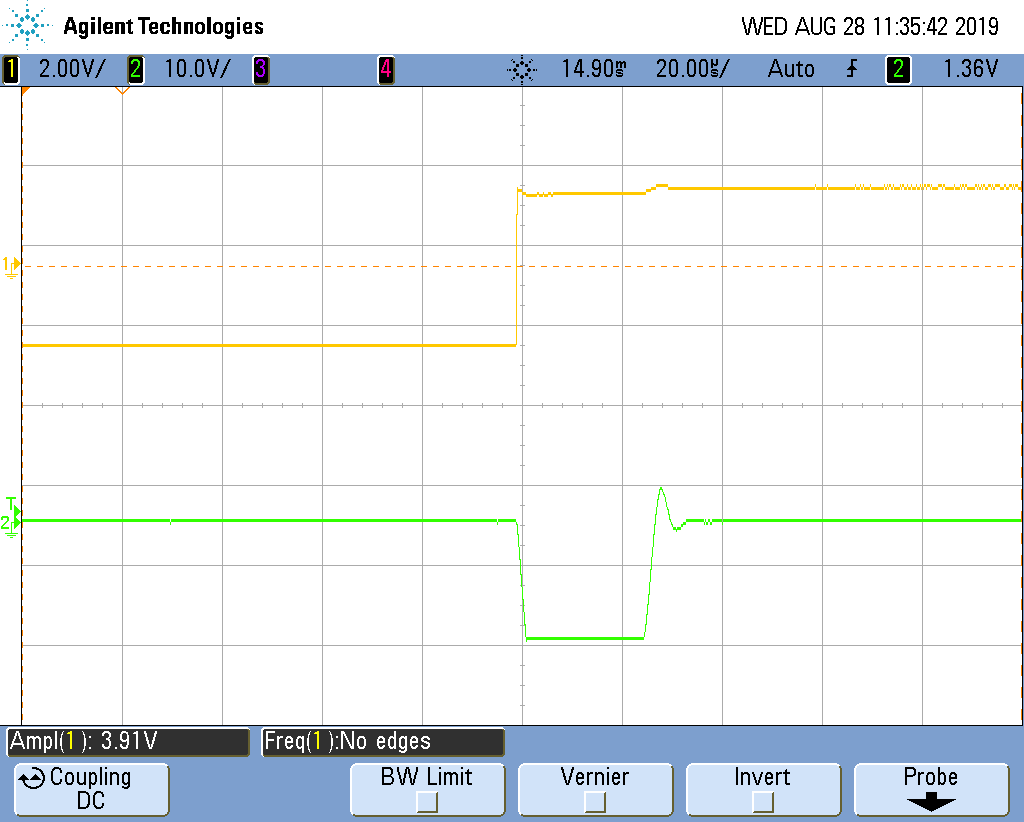
\includegraphics[scale=0.2]{Derivador/Mediciones/Osciloscopio/PCB_Compensado/Calibracion/scope_15.png} 
	\caption{Calibraci\'on del sistema desde el estado subamortiguado al cr\'iticamente amortiguado}
	\label{fig:calibracion_derivador}
\end{figure}

La figura \ref{fig:calibracion_derivador} muestra la realizaci\'on pr\'actica de la calibraci\'on propuesta, donde para la se\~nal amarilla de entrada, sea un escal\'on,
se produce una salida que se encuentra saturada y corresponde a un delta de dirac que idealmente debiera de tender a infinito. Utilizando la base de tiempo retardada del osciloscopio, se hace
zoom sobre la respuesta transitoria del sistema y se calibra tal cual fue descripto previamente hasta llegar al estado cr\'iticamente amortiguado.

\paragraph*{Impedancia de entrada con $A_{vol}$ finito} agregar una nueva resistencia en la entrada del circuito modifica la impedancia de entrada, de forma tal que el an\'alisis se puede aplicar de igual forma que para cuando no estaba, sumandole al resultado obtenido para el derivador sin compensar la resistencia adicional. Realizando algunos pasos algebraicos, se obtiene que:

\begin{figure}[H]
	\centering
	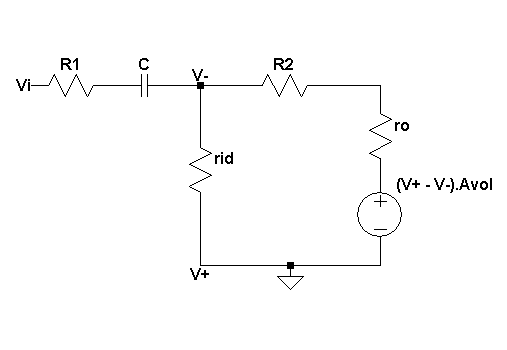
\includegraphics[scale=0.75]{Recursos/Derivador_compensado/Compensado_modelo_impedancia.png}
	\caption{Modelo equivalente del circuito incluyendo compensaci\'on}
	\label{fig:derivador_compensado_modelo}
\end{figure}

\begin{equation}
	Z_{in}(s) = \frac{1 + s \cdot C  \cdot R_1}{s \cdot C} \cdot \frac{1 + s \cdot \frac{R_1 \cdot C \cdot \left[ 2 \cdot (R_2 + Z_o) + r_{id} \cdot(1 + A_{vol}) \right]}{R_2 + Z_o + r_{id} \cdot (1 + A_{vol})}}{1 + s \cdot \frac{R_1 \cdot C \cdot \left[ (R_2 + Z_o) \cdot 2 + r_{id} \cdot ( 1 + A_{vol}) \right] - C \cdot r_{id} \cdot ( R_2 + Z_o)}{R_2 + Z_o + r_{id} \cdot(1+A_{vol})}}
\end{equation}


\paragraph*{Impedancia de entrada con polo dominante} de igual forma que para el caso anterior, se utilizan los c\'alculos realizados previamente para el circuito derivador sin compensar y luego agrega sumando la resistencia adicional en la entrada del circuito, obteniendo luego de algunos pasos algebraicos la impedancia de entrada para el caso donde se considera el polo dominante:

\begin{align*}
	Z_{in}(s) & = \frac{1}{s \cdot C} \cdot \frac{1 + s \cdot \alpha + s^{2} \cdot \beta}{1 + s \cdot \frac{r_{id} + r_{o} + R_2}{\omega_p \cdot \left[ (A_o + 1 ) \cdot r_{id} + r_o + R_2 \right]}} \\
	\alpha & = \frac{r_{id} + R_2 + r_o + \omega_p \cdot C \cdot \left[ r_{id} \cdot ( R_2 + r_o) + R_1 \cdot(r_{id} \cdot ( A_o + 1) + r_o + R_2) \right] }{\omega_p \cdot \left[ r_o + R_2 + r_{id} \cdot (A_o + 1) \right]} \\
	\beta & = \frac{C \cdot \left[ r{id} \cdot ( R_2 + r_o ) + R_1 \cdot (r_{id} + r_o + R_2)) \right]}{\omega_p \cdot \left[ R_2 + r_o + r_{id} \cdot (A_o + 1) \right] }
\end{align*}

\paragraph*{Expresiones finales} de las expresiones te\'oricas obtenidas para el derivador compensado y luego de realizar el dise\~no para cumplir con los criterios impuestos, considerando que el preset calibrado estar\'a en el entorno de $R_1 = 103,487$, se obtienen las expresiones con valores num\'ericos para realizar las comparaciones te\'oricas. Vale aclarar que en la pr\'actica el preset no tendr\'a dicho valor, sino que la suma entre las resistencia de entrada del generador, las par\'asitas y la del preset dar\'an tal resultado.

\begin{equation}
	H(s) = - \frac{\frac{s}{10000,1}}{1 + s \cdot 2,08 \cdot 10^{-6} + \left( \frac{s}{2\pi \cdot 152,935 kHz}\right)^{2}}
\end{equation}

\begin{equation}
	Z_{in}(s) = \frac{1 + \frac{s}{2\pi \cdot 76,89kHz}}{\frac{s}{2\pi 7,95MHz}} \cdot 
	\frac{1 + s \cdot 2,0806 \cdot 10 ^{-6} + \left( \frac{s}{2\pi \cdot 1,04MHz} \right)^{2}}{1 + s \cdot 2,076 \cdot 10^{-6} - \left( \frac{s}{2 \pi \cdot 155,64kHz} \right)^{2}}
\end{equation}

\subsubsection{Resultados}
En esta secci\'on se realizan las simulaciones, mediciones correspondientes sobre el circuito y se contrastan dicho resultados
con los valores te\'oricos, con el objetivo de determinar la efectividad del circuito propuesto como derivador, y su rango de operaci\'on.

\paragraph*{Respuesta en frecuencia} en el gr\'afico del m\'odulo de la respuesta en frecuencia se pueden observar cuatro conjuntos de curvas
que son f\'acilmente reconocibles como la te\'orica, la medida, y las simuladas. En primer lugar, es necesario prestar atenci\'on a la diferencia entre el resultado
te\'orico y la medici\'on, claramente lo obtenido no cumple con el requisito impuesto donde se buscaba un sistema subamortiguado, ya que se puede observar que la medici\'on 
tiene un ligero sobrepico. No obstante, esta diferencia se debe al hecho de que, si bien el sistema como tal se encuentra cr\'iticamente amortiguado pues fue calibrado analizando
la respuesta transitoria del mismo, la diferencia entre teor\'ia y pr\'actica yace en qu\'e se est\'a midiendo. El an\'alisis te\'orico supone un generador de funciones ideal
sin impedancia en serie, con lo cual la caracterizaci\'on del sistema es directamente estableciendo $H(s) = \frac{V_o}{V_{gen}}$, no obstante en la pr\'actica el generador tiene una resistencia
en serie de $R = 50 \Omega$ y lo que en verdad se est\'a midiendo es $H(s) = \frac{V_o}{V_i}$. Esta diferencia implica que el sistema que fue calibrado como cr\'ticamente amortiguado se compone, conceptualmente,
de una resistencia de compensaci\'on resultante de la agrupaci\'on serie entre el preset y la resistencia del generador.

\begin{figure}[H]
	\centering
	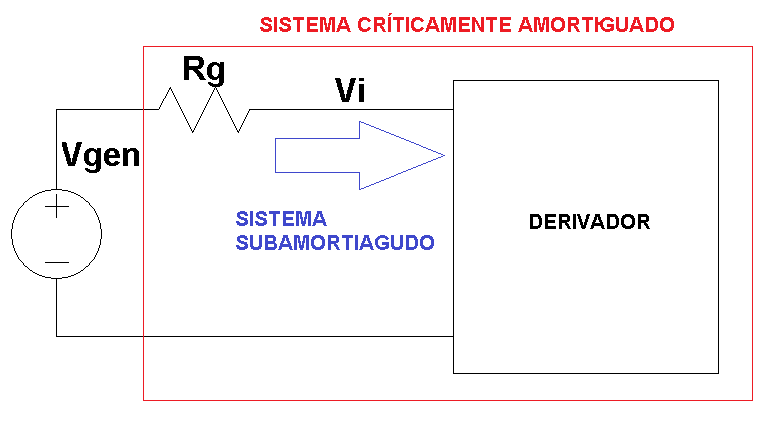
\includegraphics[scale=0.6]{Recursos/Integrador/correccion.png}
	\caption{Diagrama explicativo del error cometido en el dise\~no}
	\label{fig:derivador_correccion}
\end{figure}

Analizando con mayor detalle, los resultados no implican en verdad que haya habido un error, solamente indican
un subamortiguamiento que no caracteriza al sistema que en verdad se debe considerar. Concluyendo, si se caracteriza al sistema a partir de las se\~nales de entrada
y salida que pueden ser medidas, se termina describiendo un sistema subamortiguado que no es el que est\'a siendo puesto a prueba ya que el que verdaderamente es empleado a la hora de derivar se\~nales est\'a cr\'ticamente
amortiguado y su respuesta en frecuencia no puede ser caracterizada, pues ser\'ia necesario medir directamente sobre la $V_{gen}$ del modelo propuesto. Por esto \'ultimo es que se considera que el
m\'etodo de calibraci\'on analizando la respuesta temporal es la mejor forma de observar que el sistema se encuentra cr\'iticamente amortiguado.

\begin{figure}[H]
	\centering
	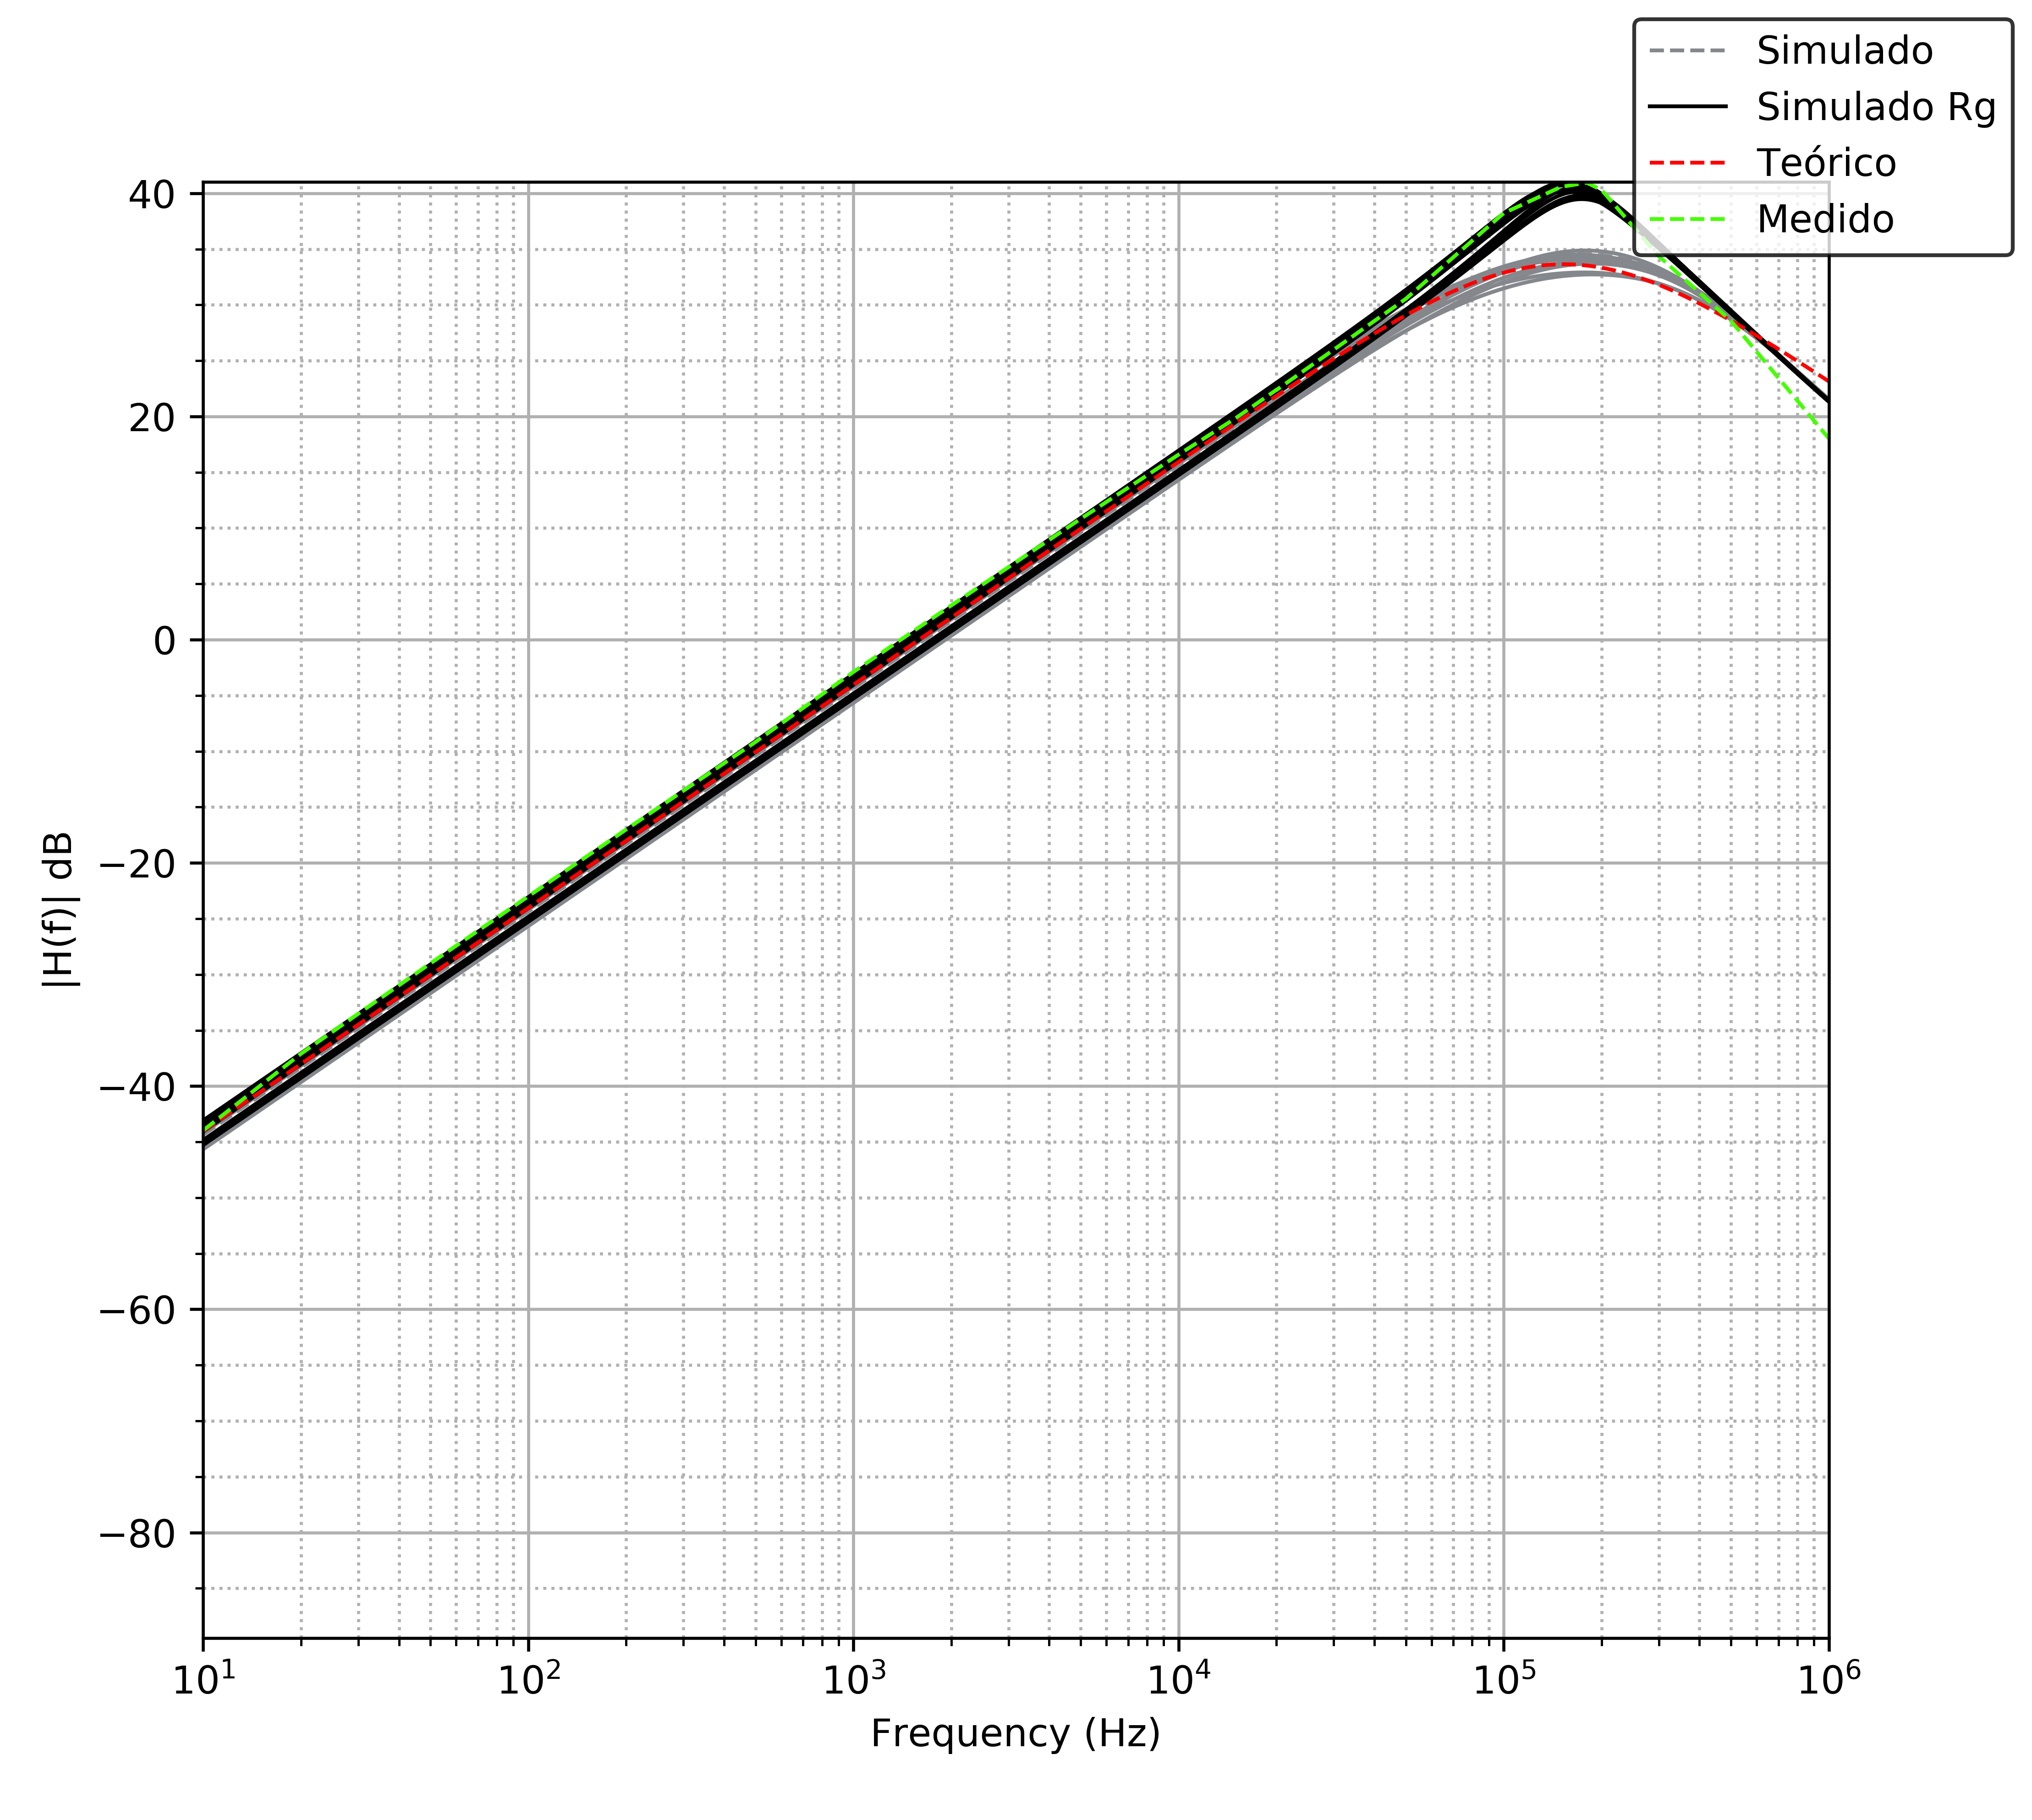
\includegraphics[scale=0.6]{Recursos/Derivador_compensado/bode_modulo.png}
	\caption{Diagrama de bode en m\'odulo del derivador compensado}
	\label{fig:derivador_compensado_bode_modulo}
\end{figure}

\begin{figure}[H]
	\centering
	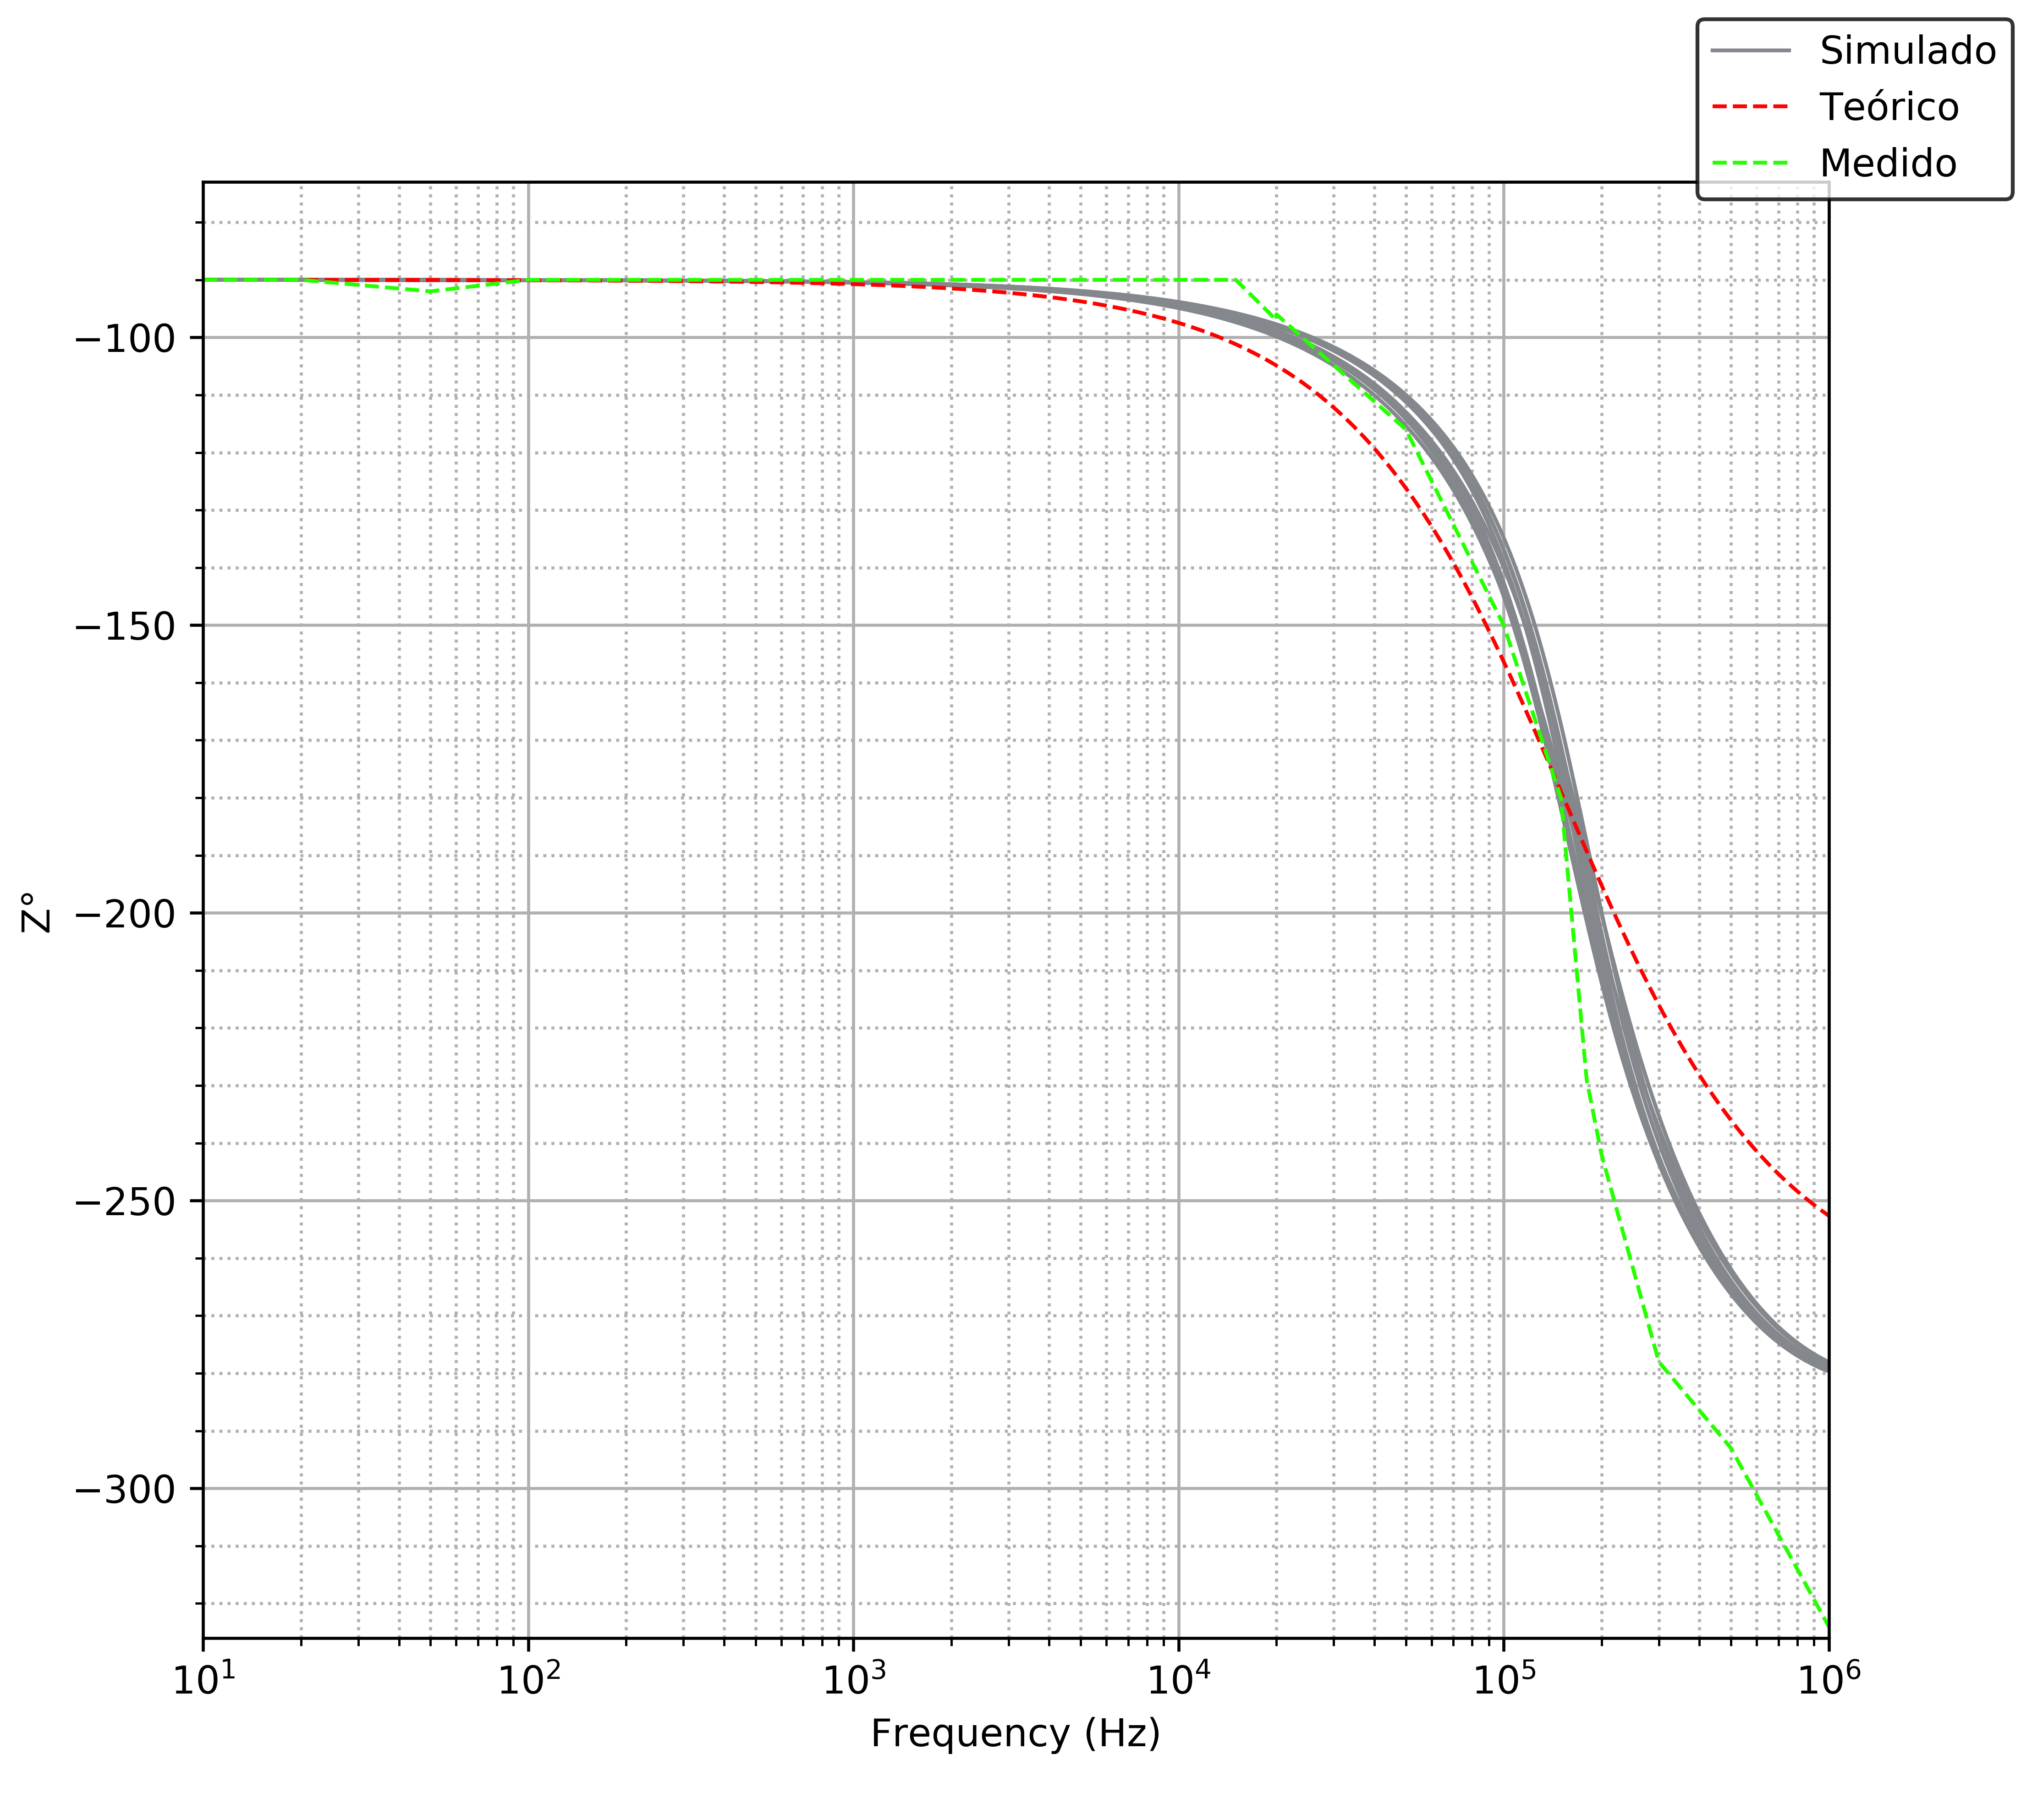
\includegraphics[scale=0.6]{Recursos/Derivador_compensado/bode_fase.png}
	\caption{Diagrama de bode en fase del derivador compensado}
	\label{fig:derivador_compensado_bode_fase}
\end{figure}

Finalmente, en principio se puede observar que por el diagrama de bode en fase que se obtuvo de las mediciones,
el circuito puede considerarse derivador hasta una frecuencia aproximadamente de $f_{max} = 15kHz$, donde como se puede
observar a continuaci\'on, si se quisiera que la tensi\'on pico a pico de la se\~nal de entrada permaneciera constante para toda
frecuencia, deberia utilizarse como m\'aximo $V_pp = 2,91 V$ para evitar saturaci\'on de la salida. Estas conclusiones se obtienen de los datos
utilizados para las gr\'aficas realizadas, t\'engase en cuenta que se fueron tomando valores de tensi\'on y frecuencia en los cuales no se produc\'ia
ninguna distorsi\'on o deformaci\'on de la salida, siempre y cuando lo obtenido diera como resultado una medici\'on apreciable.

\begin{table}[H]
	\centering
	\begin{tabular}{c c c c c}%
		$V_{gen} [V]$ & $f_{gen} [Hz]$ & $V_{out} [V]$ & $\phase{V_{out}} [\circ]$ & $\frac{V_o}{V_i} [dB]$ \\ \hline
		\csvreader[head to column names, late after line=\\]{bode_derivador_compensado.csv}{}{\gen & \f & \out & \p & \db}
		\hline
	\end{tabular}
\end{table}

\paragraph*{Impedancia de entrada} como se puede observar, las curvas te\'oricas, medidas y simuladas contrastan bien salvo
por diferencias en el m\'odulo en torno a la frecuencia de corte del cero de segundo orden. Esto \'ultimo se justifica de la misma forma que sucedi\' con la 
respuesta en frecuencia, ya que en las mediciones se posee una resistencia del generador que modifica el comportamiento del sistema que efectivamente se mide,
y por ello se puede apreciar que la medici\'on tiene un valor mucho menor que el caso cr\'iticamente amortiguado de la teor\'ia.

\begin{figure}[H]
	\centering
	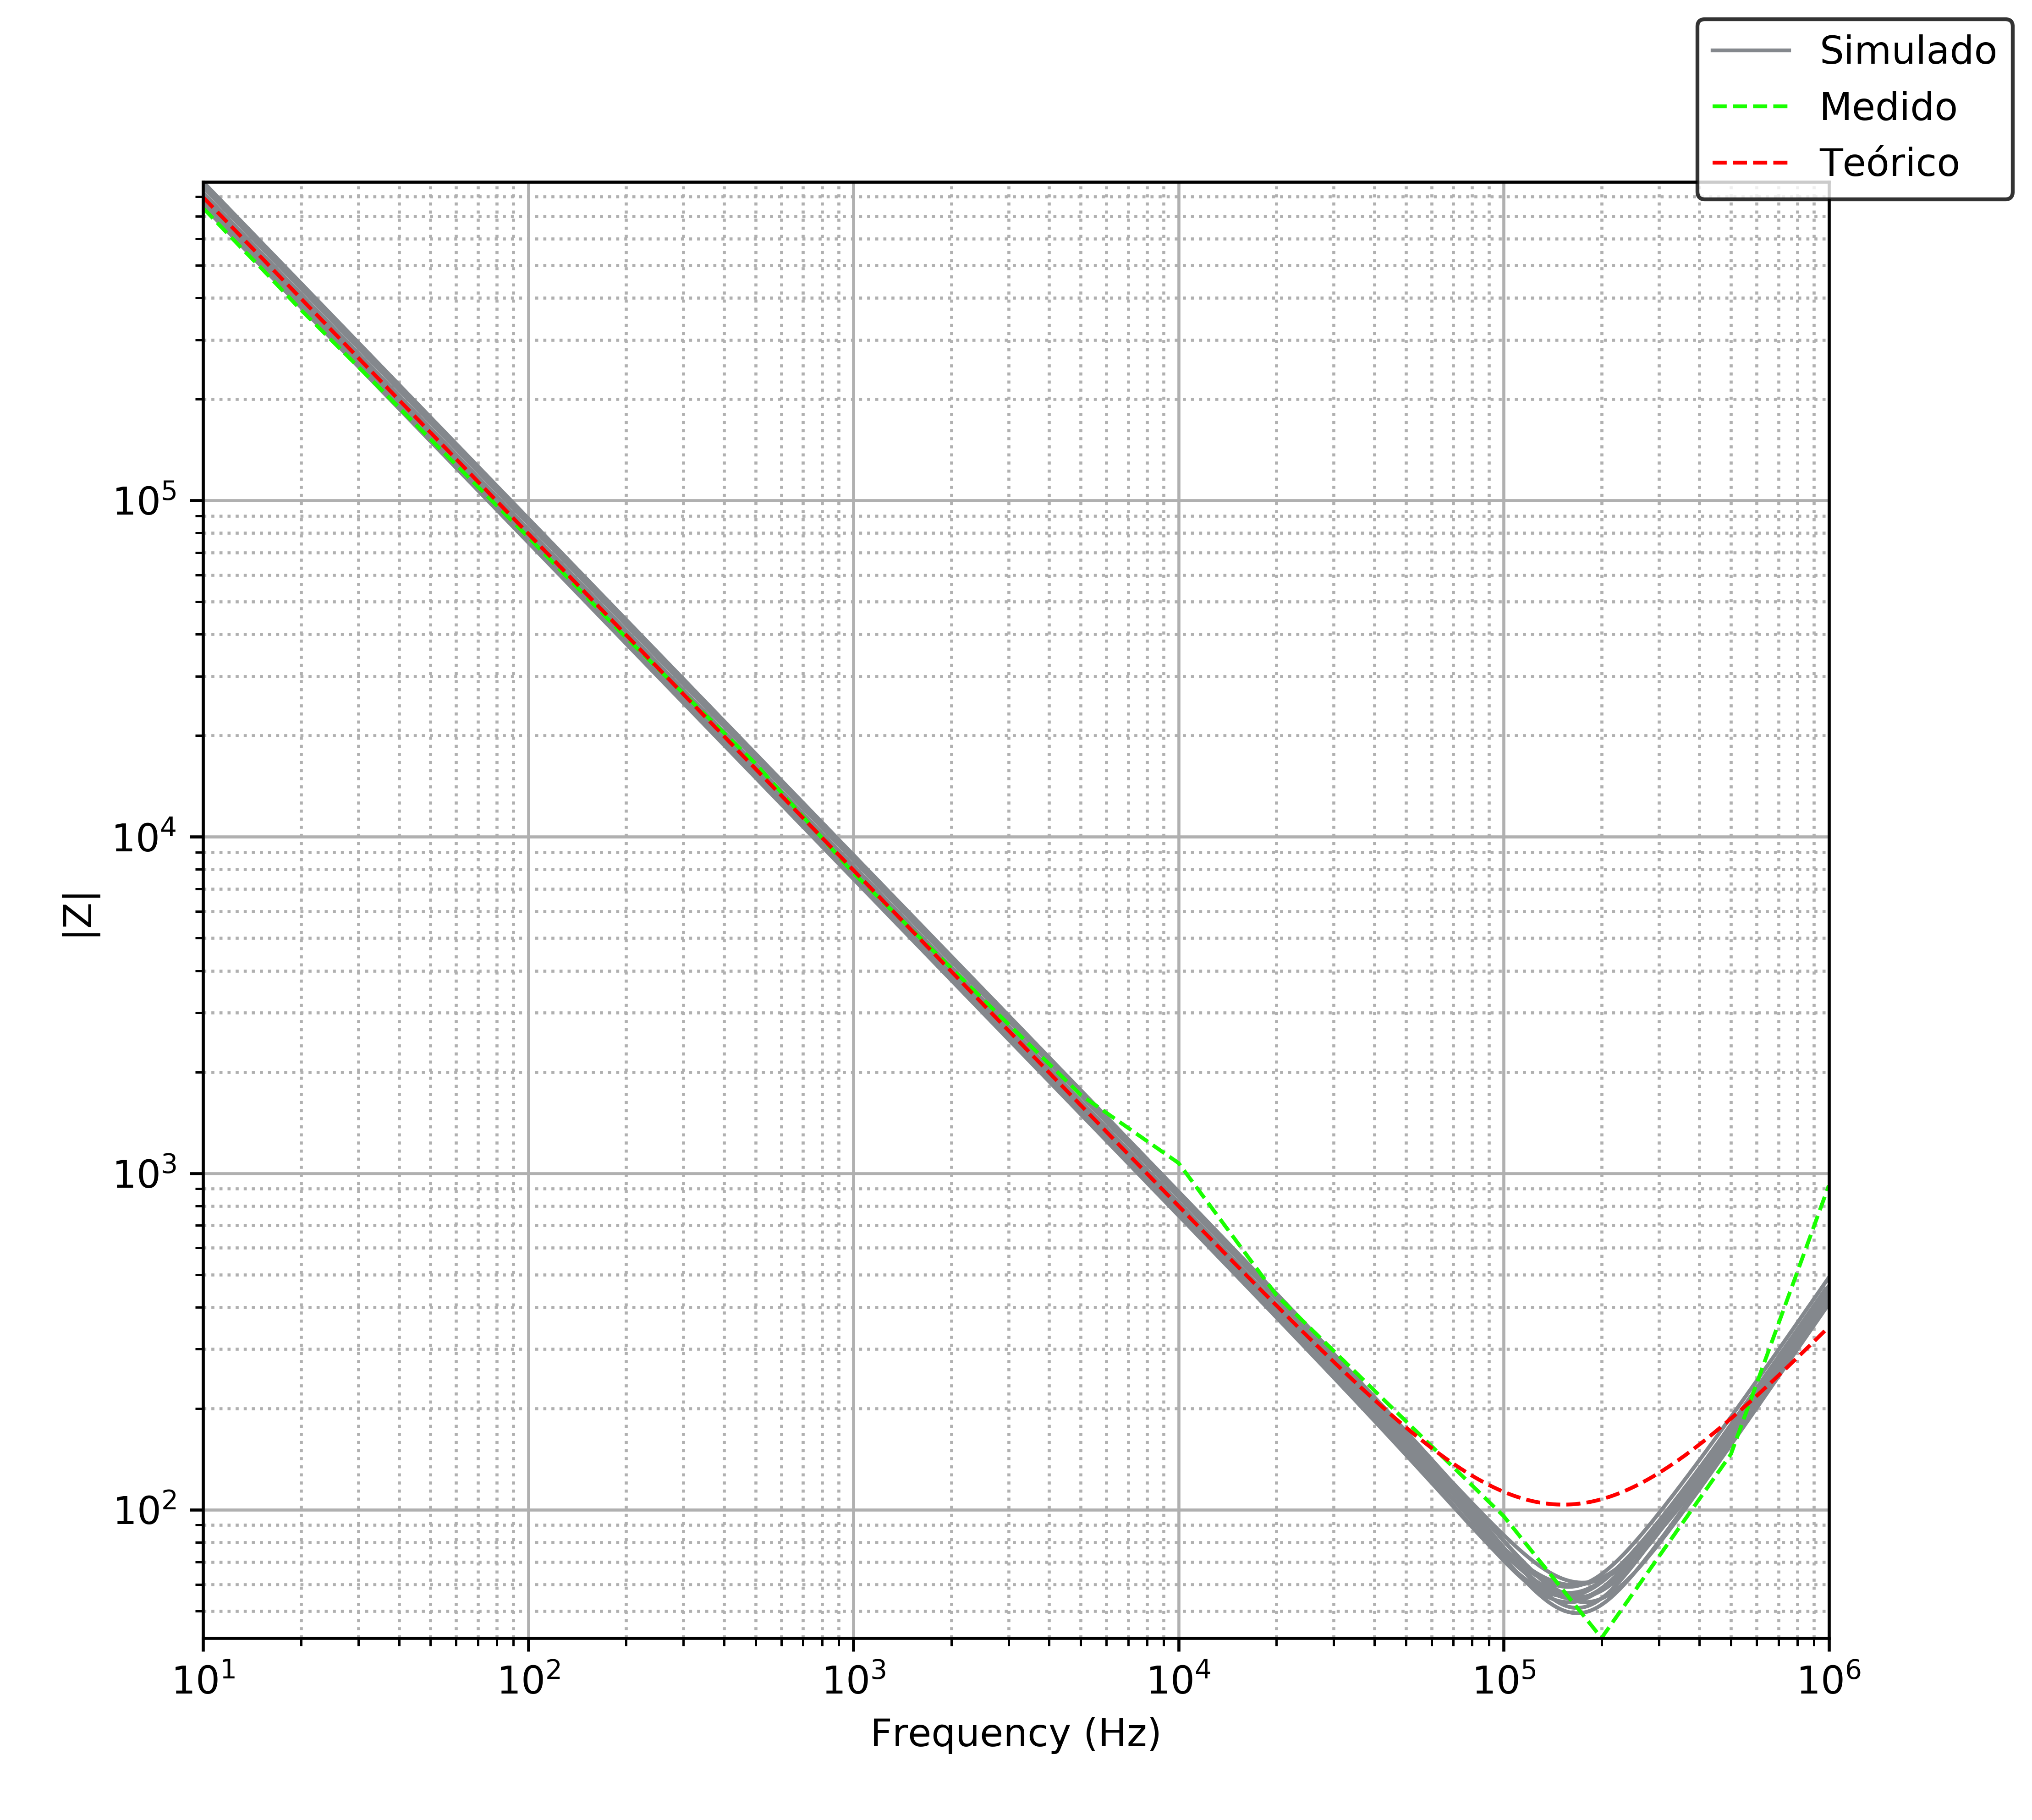
\includegraphics[scale=0.7]{Recursos/Derivador_compensado/impedancia_modulo.png}
	\caption{Impedancia de entrada del derivador compensado, en modulo}
	\label{fig:derivador_compensado_impedancia_modulo}
\end{figure}

\begin{figure}[H]
	\centering
	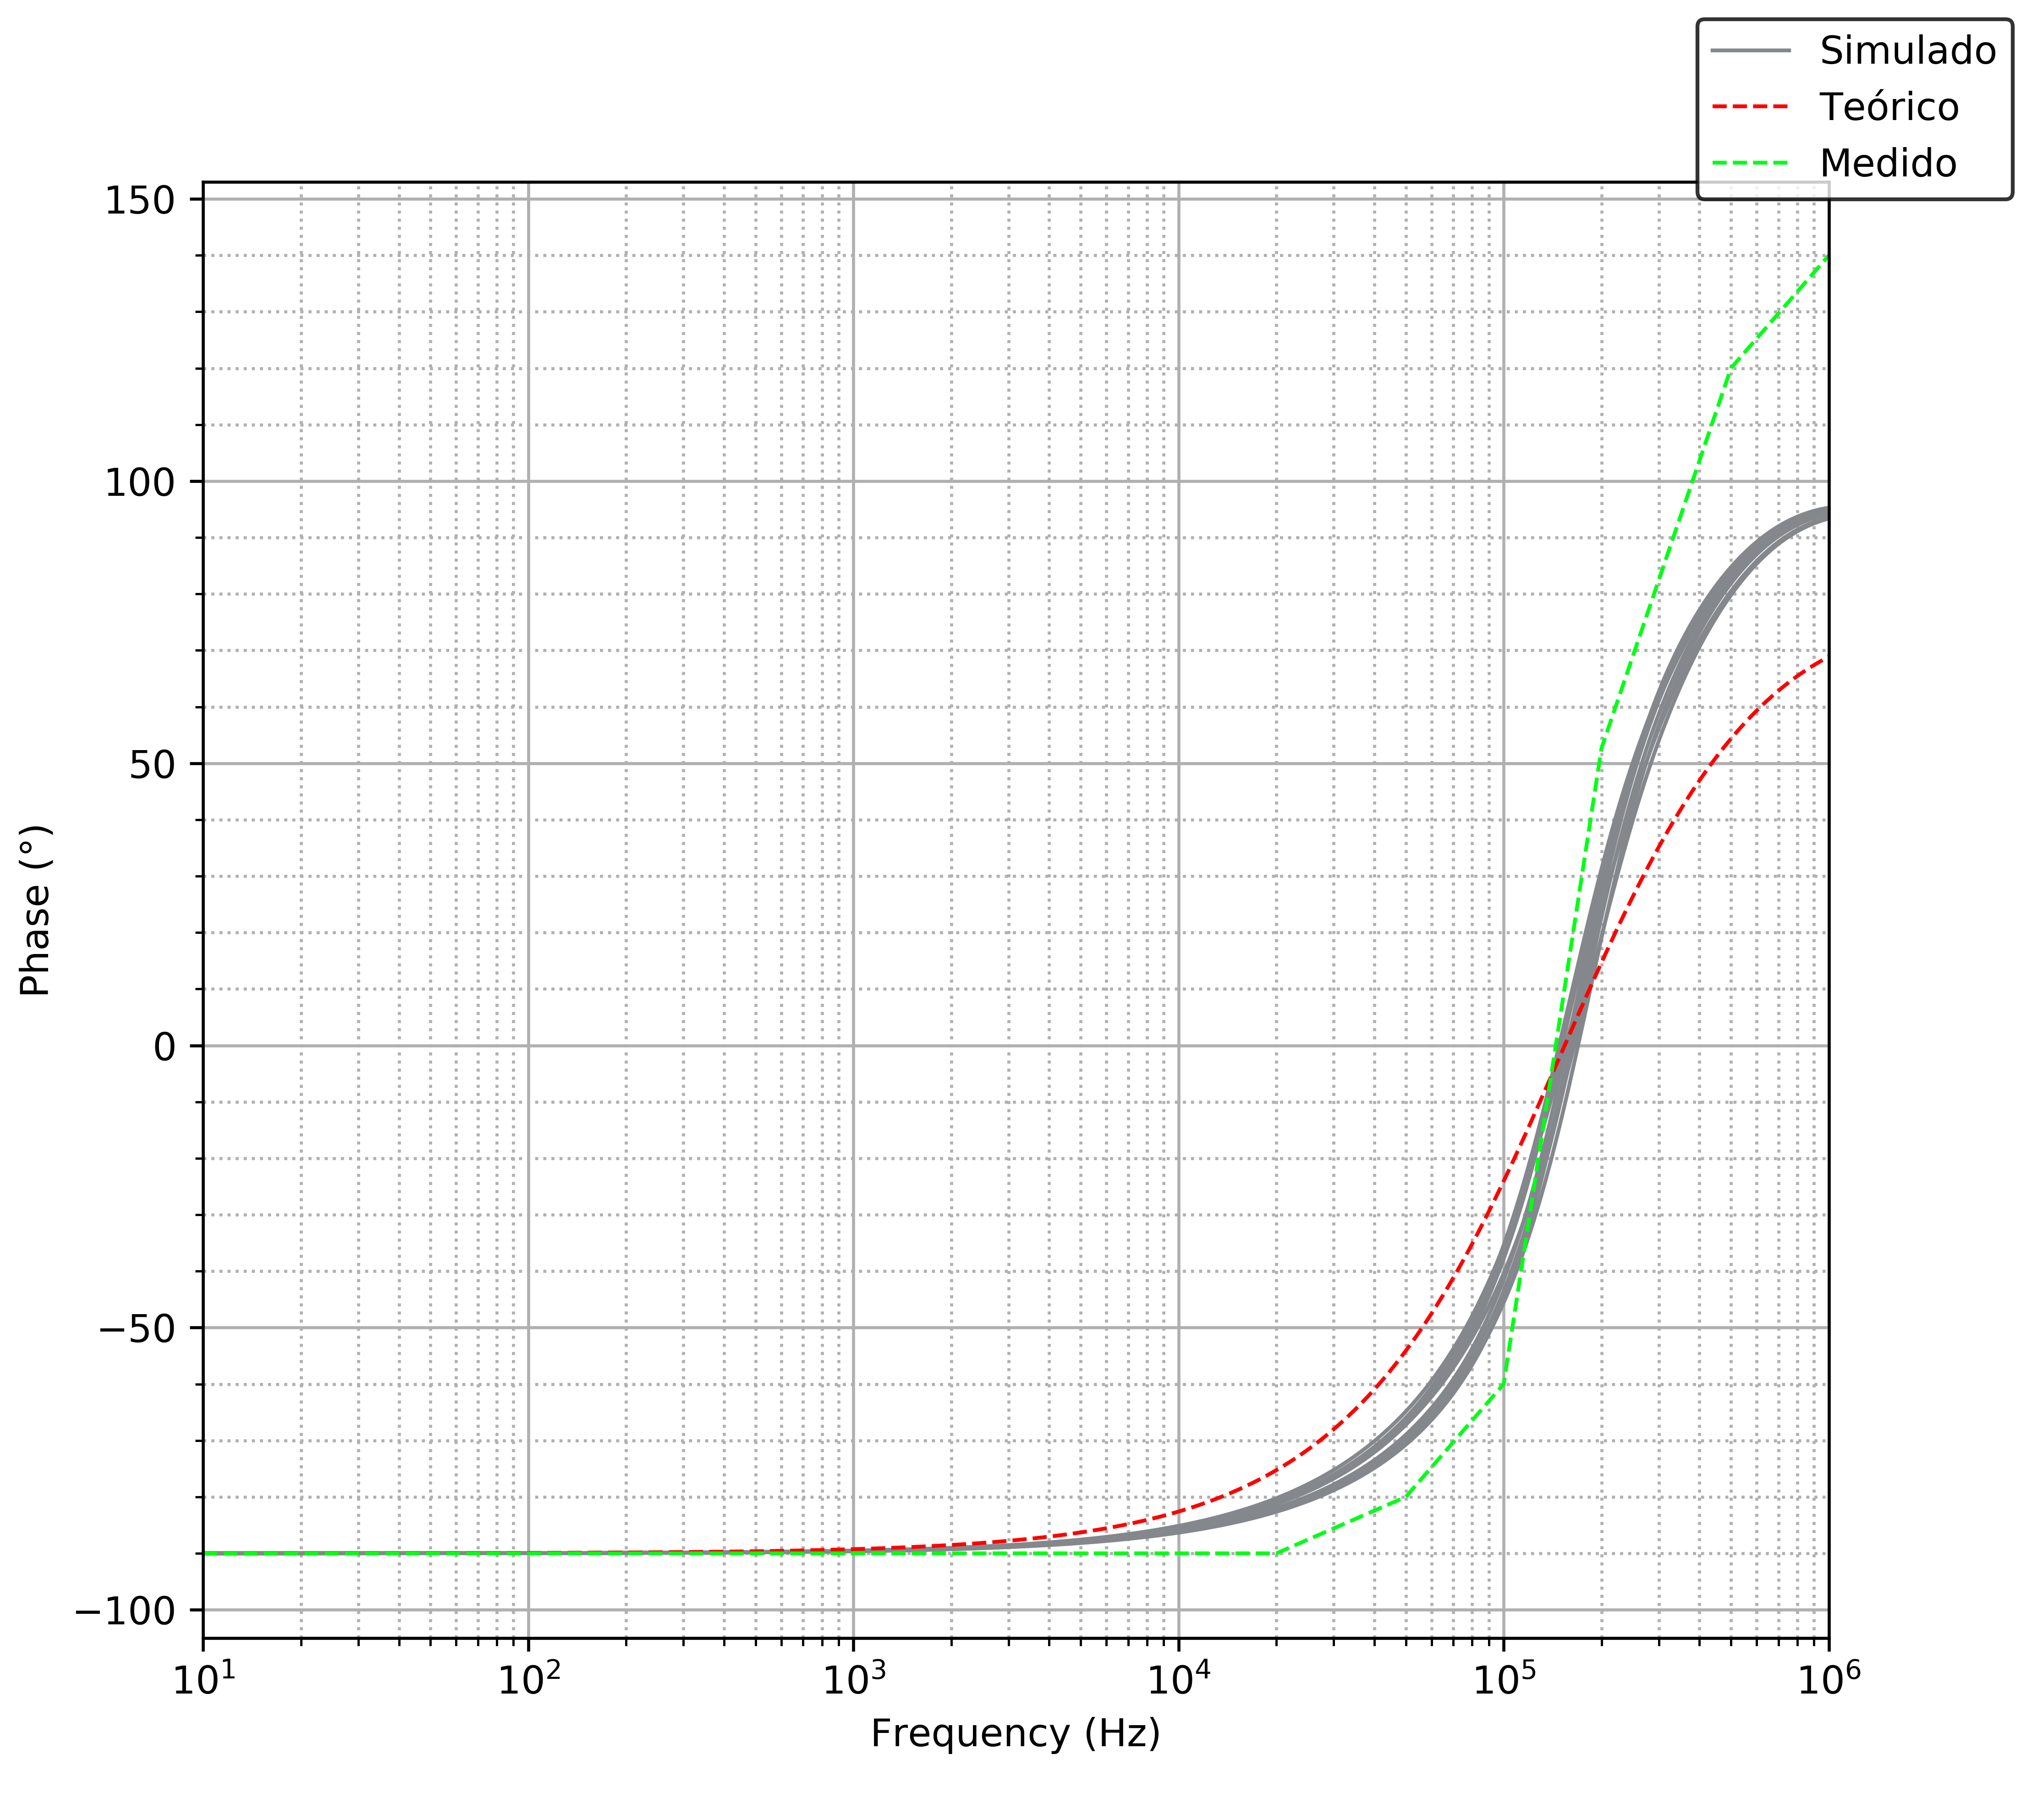
\includegraphics[scale=0.7]{Recursos/Derivador_compensado/impedancia_fase.png}
	\caption{Impedancia de entrada del derivador compensado, en fase}
	\label{fig_derivador_compensado_impedancia_fase}
\end{figure}

\paragraph*{Respuesta a se\~nales no senoidales} en las curvas ilustradas, las amarillas corresponden a las se\~nales de entrada y las verdes
a las se\~nales de salida.

\begin{figure}[H]
	\centering
	\begin{tabular}{c c}
		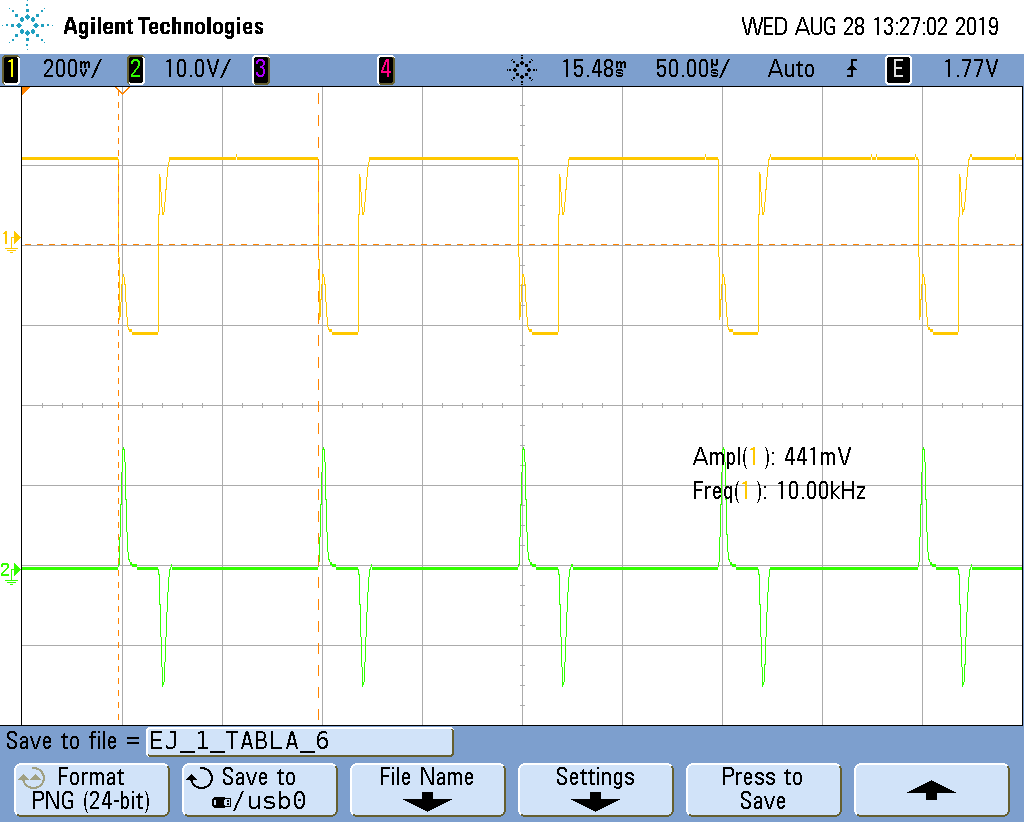
\includegraphics[scale=0.2]{Derivador/Mediciones/Osciloscopio/PCB_Compensado/EJ_1_TABLA_6.png} &
		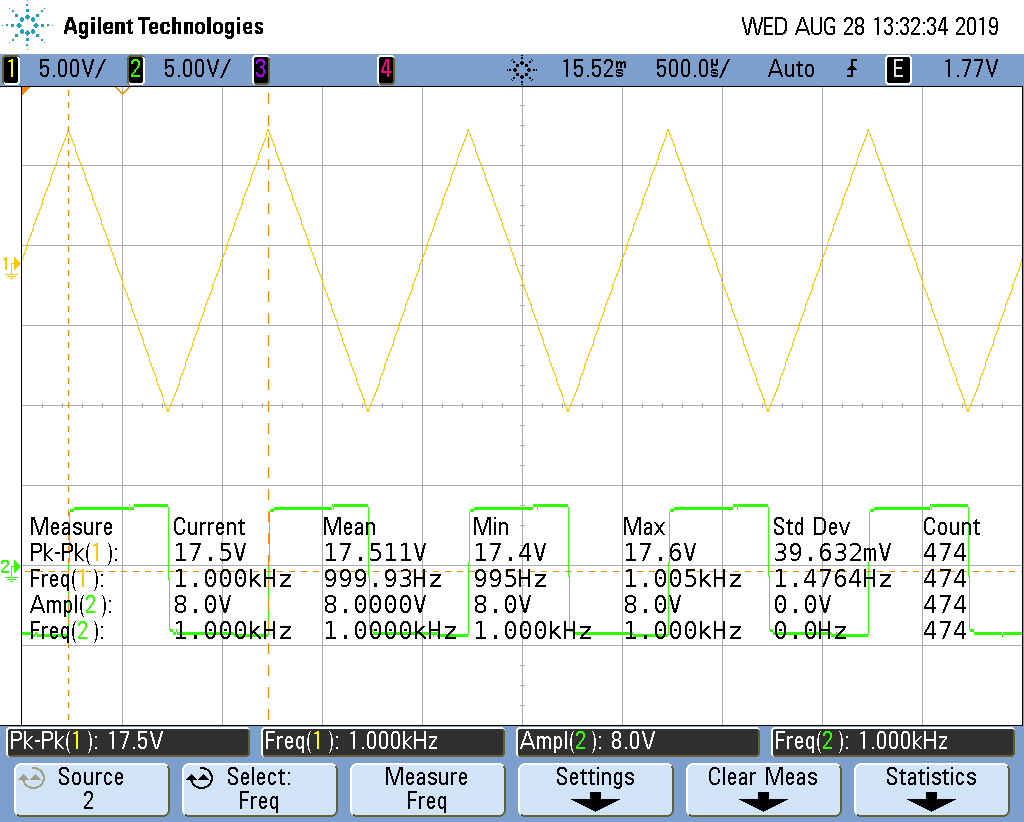
\includegraphics[scale=0.2]{Derivador/Mediciones/Osciloscopio/PCB_Compensado/osc_4.png} \\
		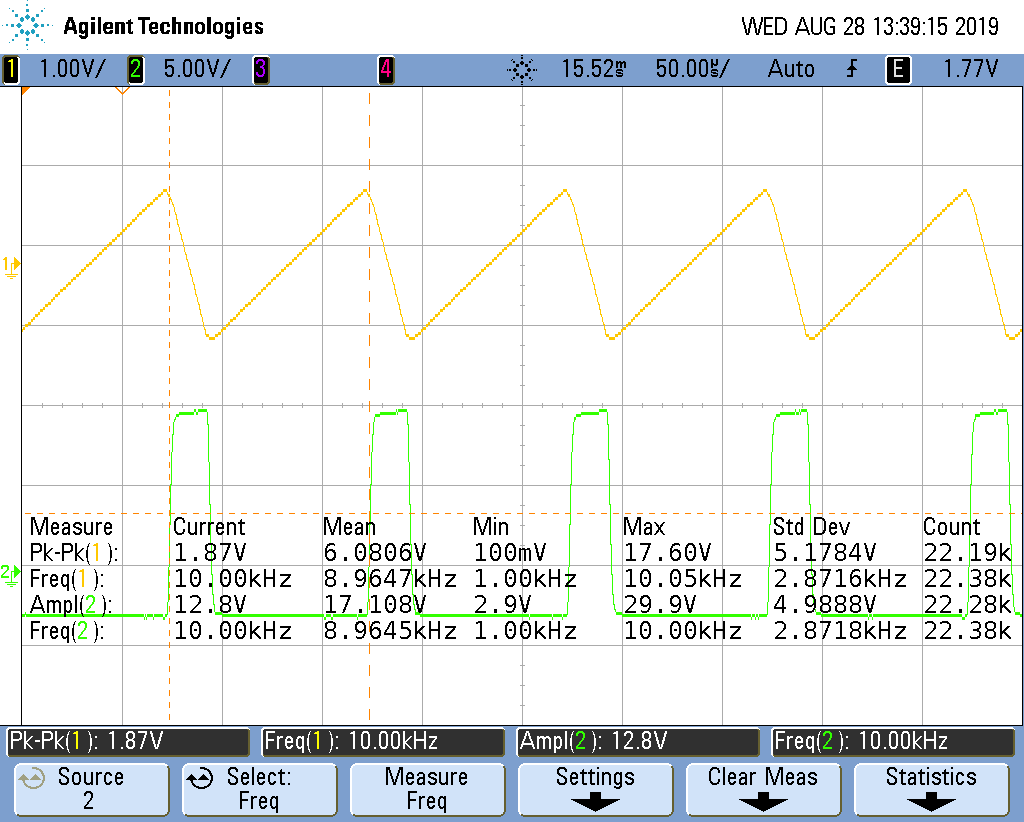
\includegraphics[scale=0.2]{Derivador/Mediciones/Osciloscopio/PCB_Compensado/osc_8.png} &
		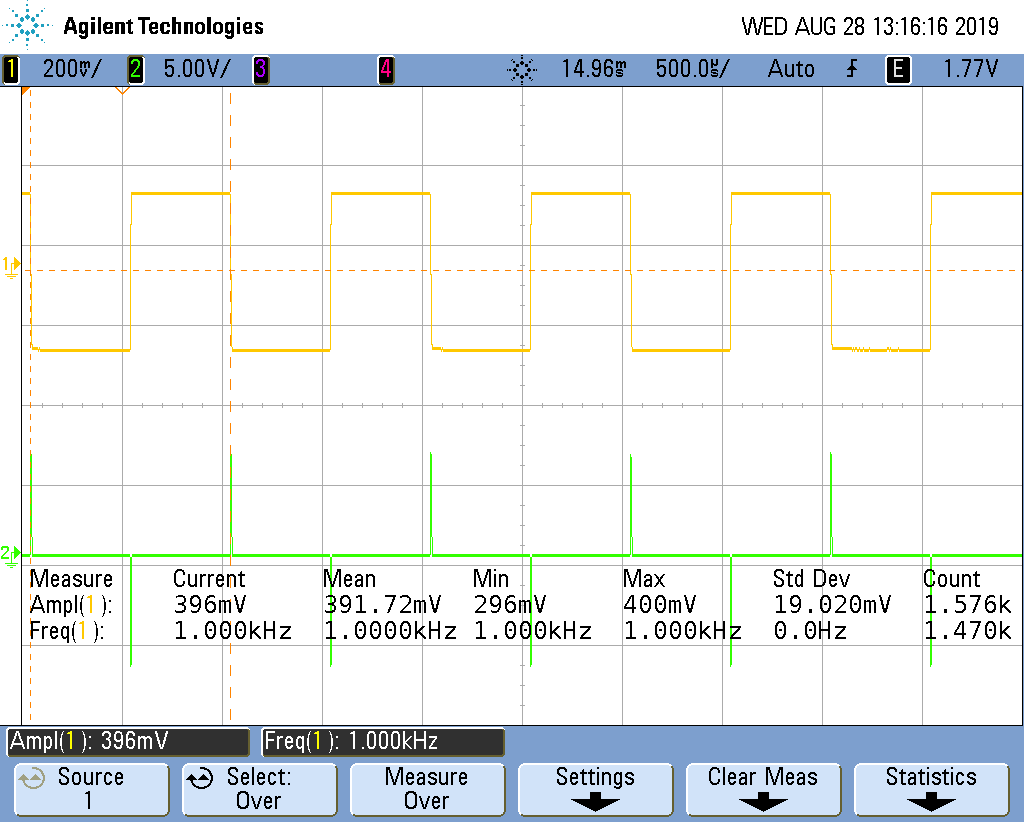
\includegraphics[scale=0.2]{Derivador/Mediciones/Osciloscopio/PCB_Compensado/scope_23.png} 
	\end{tabular}
	\caption{Medici\'on de respuesta a se\~nales no senoidales}
	\label{fig:respuesta_derivador_compensado}
\end{figure}

	\subsection{Circuito integrador}

\begin{figure}[H]
	\centering
	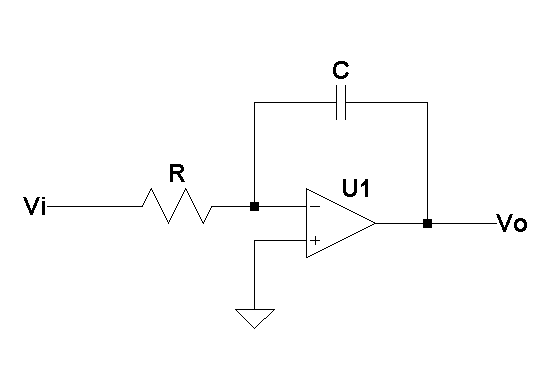
\includegraphics[scale=0.8]{Recursos/Integrador/Circuito_integrador.png}
	\caption{Circuito integrador sin compensar}
	\label{fig:circuito_integrador}
\end{figure}
\subsubsection{An\'alisis Te\'orico}

\paragraph*{Funci\'on transferencia en condiciones ideales} considerando el sistema LTI, causal y bibo-estable, bajo condiciones de idealidad donde $A_{vol} \rightarrow \infty$, luego como se conoce la expresi\'on para dicho caso del amplificador inversor, se obtiene que:
<<<<<<< HEAD

\begin{equation}
	H(s) = - \frac{\frac{1}{s \cdot C}}{R} = - \frac{1}{s \cdot C \cdot R}
	\Rightarrow
	H(s) = - \frac{1}{\frac{s}{2 \pi \cdot 1,591kHz}}
	\label{eq:integrador_transfer_ideal}
\end{equation}

En este primer acercamiento al comportamiento del circuito, se puede observar en la funci\'on transferencia que se describe un sistema que no es bibo-estable como se asumi\'o en un principio, sino que posee un polo en el origen. Esto \'ultimo tiene sentido porque implica que para entradas acotadas, la respuesta ser\'a la integral de dicha entrada acotada, pudiendo dar un resultado no acotado en el tiempo. Desde otro punto de vista, para frecuencias muy bajas o se\~nales continuas, la impedancia del capacitor en la realimentaci\'on es demasiado grande y provoca una desconexi\'on o un lazo d\'ebil, por lo tanto el amplificador operacional satura puesto que amplifica en t\'erminos de su $A_{vol}$ correspondiente seg\'un sea el caso.

\paragraph*{Funci\'on transferencia con $A_{vol}$ finito} consid\'erese un $A_{vol}$ finito, luego se plantean los valores de potencial el\'ectrico sobre los terminales de las entradas del amplificador operacional y se calcula la salida con la ecuaci\'on correspondiente al modelo del mismo. Entonces, se obtiene:

\begin{equation*}
	v^{-} = V_i \cdot \frac{\frac{1}{s \cdot C}}{\frac{1}{s \cdot C} + R} + V_o \cdot \frac{R}{\frac{1}{s \cdot C} + R}
	\Rightarrow
	v^{-} = \frac{V_i + V_o \cdot s \cdot C \cdot R}{1 + s \cdot C \cdot R}
\end{equation*}

\begin{equation*}
	V_o = (v^{+} - v^{-}) \cdot A_{vol} \Rightarrow
	V_o \cdot \left[ 1 + \frac{A_{vol} \cdot s \cdot R \cdot C}{1 + s \cdot C \cdot R} \right] =
	- V_i \cdot \frac{A_{vol}}{1 + s \cdot C \cdot R}
\end{equation*}

\begin{equation}
	H(s) = \frac{V_o(s)}{V_i(s)} = \frac{-A_{vol}}{1 + s \cdot C \cdot R \cdot (A_{vol} + 1)}
	\Rightarrow
	H(s) = \frac{-100000}{1 + \frac{s}{2 \pi \cdot 0,0159Hz}}
	\label{eq:integrador_transfer_avol_finito}
\end{equation}

Se puede observar que con estas nuevas consideraciones, el sistema dej\'o de ser inestable en t\'erminos de su respuesta, no obstante sigue sucediendo que para frecuencias muy bajas la realimentaci\'on pasa a tener un lazo d\'ebil y satura el amplificador operacional.

\paragraph*{Funci\'on transferencia con polo dominante} ahora se considera que la ganancia del amplificador operacional tiene el polo dominante, con lo cual no se mantiene invariante en frecuencia. Reutilizando la expresi\'on anterior para $A_{vol}$ finito y reemplazando tal t\'ermino por la expresi\'on con el polo dominante se obtiene:

\begin{equation*}
	H(s) = - \frac{A_o \cdot \omega_p}{s + \omega_p + s \cdot C \cdot R \cdot (A_o \cdot \omega_p + s + \omega_p)}
	\Rightarrow
	H(s) = - \frac{A_o}{1 + s \cdot \frac{1 + C \cdot R \cdot \omega_p \cdot ( A_o + 1 )}{\omega_p} + s^{2} \cdot \frac{C \cdot R}{\omega_p}}
\end{equation*}

\begin{equation*}
	H(s) = - \frac{100000}{1 + s \cdot 10,001 + \left( \frac{s}{2 \pi \cdot 488,60Hz} \right)^{2}}
\end{equation*}

En esta nueva expresi\'on de la funci\'on transferencia, el sistema refleja un segundo orden en el denominador del cual se pueden determinar los par\'ametros caracter\'isticos del mismo, obteniendo que $\omega_o = 3069,96 \frac{1}{s}$ y $\xi = 15351,58 \geq 1$. Entonces el sistema se encuentra en un sobreamortiguamiento con frecuencias de corte ubicadas en $f_1 = 15,0017MHz$ y $f_2 = 0,01499Hz$.

\begin{equation}
	H(s) = - \frac{106092,66}{(1 + \frac{s}{2 \pi \cdot 0,014998Hz}) \cdot (1 + \frac{s}{2 \pi \cdot 15,0017MHz})}
	\label{eq:integrador_transfer_polo_dominante}
\end{equation}

En este nuevo resultado la \'unica diferencia con respecto al anterior, es que ahora hay un polo adicional que aparece en una frecuencia muy alejada, no obstante sigue saturando para frecuencias muy bajas por el lazo d\'ebil, es por esto que este circuito no funcionar\'a correctamente con el prop\'osito para el que fue pensado desde un punto de vista ideal, por ende ser\'a necesario realizar alguna compensaci\'on para poder corregirlo.

\paragraph*{Impedancia de entrada con $A_{vol}$ finito} para encontrar la impedancia de entrada considerando el $A_{vol}$ finito, se redibuja el circuito reemplazando al amplificador operacional con su circuito equivalente y se plantea la ley de nodos.
Se llama a la diferencia de potencial $V_d = V^{+} - V^{-}$.

\begin{figure}[H]
	\centering
	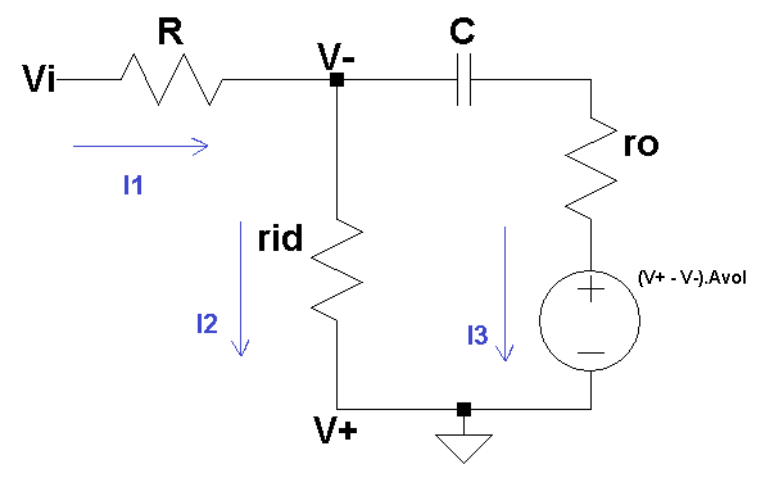
\includegraphics[scale=0.7]{Recursos/Integrador/Circuito_integrador_modelo_impedancia.png}
	\caption{Circuito equivalente para c\'alculo de impedancia de entrada}
	\label{fig:integrador_modelo}
\end{figure}

\begin{equation*}
	I_1 = I_2 + I_3 \Rightarrow
	\frac{V_i + V_d}{R_1} = 
	\frac{-V_i}{R_1} + \frac{- V_i - V_i \cdot A_{vol}}{\frac{1}{s \cdot C} + R}
\end{equation*}

\begin{equation*}
	V_d = \frac{- V_i \cdot r_i \cdot ( 1 + s \cdot C \cdot Z_o)}{r_i \cdot(s \cdot C \cdot Z_o + 1) + R_1 \cdot (1 + s \cdot C \cdot Z_o) + s \cdot C \cdot R_1 \cdot r_i \cdot (1 + A_{vol})}
\end{equation*}

\begin{equation*}
	Z_i(s) = \frac{V_i(s)}{I_1(s)} = \frac{V_i(s)}{\frac{V_i(s) + V_d(s)}{R_1}}
	\Rightarrow
	Z_i(s) = (R_1 + r_i) \cdot \frac{1 + s \cdot \frac{C \cdot \left[ Z_o \cdot (R_1 + r_i) + R_1 \cdot r_i \cdot (A_{vol} + 1) \right]}{R_1 + r_i}}{1 + s \cdot C \left[ Z_o + r_i \cdot ( 1 + A_{vol}) \right]}
\end{equation*}

\begin{equation}
	Z_i(s) = (180k \Omega) \cdot \frac{1 + \frac{s}{2 \pi \cdot 0,0163Hz}}{1 + \frac{s}{2 \pi \cdot 0,00045Hz}}
	\label{eq:integrador_impedancia_avol_finito}
\end{equation}

\paragraph*{Impedancia de entrada con polo dominante} reutilizando la expresi\'on anterior para la impedancia de entrada y considerando la variaci\'on del $A_{vol}$ respecto de la frecuencia, se obtiene:

\begin{equation*}
	Z_i(s) = (R_1 + r_i) \cdot \frac{1 + s \cdot \frac{r_i + R_1 + \omega_p \cdot C \cdot \left[ Z_o \cdot ( R_1 + r_i ) + R_1 \cdot r_i \cdot (A_o + 1) \right]}{\omega_p \cdot (R_1 +r_i)} + s^{2} \cdot \frac{C \cdot \left[ Z_o \cdot (R_1 + r_i) + R_1 \cdot r_i \right]}{\omega_p \cdot (R_1 + r_i)}}{1 + s \cdot \frac{1 + \omega_p \cdot C \cdot (Z_o + r_i \cdot ( A_o + 1 ) )}{\omega_p} + s^{2} \cdot \frac{C \cdot(Z_o + r_i)}{\omega_p}}
\end{equation*}

\begin{equation*}
	Z_i(s) = (180k \Omega) \cdot \frac{1 + s \cdot 9,723 + \left( \frac{s}{2 \pi \cdot 493,65Hz} \right)^{2}	}{1 + s \cdot 350,0045 + \left(\frac{s}{2 \pi \cdot 82,58Hz} \right)^{2}}
\end{equation*}

\begin{equation}
	Z_i(s) = 180k \Omega \cdot \frac{(1 + \frac{s}{2 \pi \cdot 25,45Hz}) \cdot (1 + \frac{s}{2 \pi \cdot 9574,06Hz})}{(1 + \frac{s}{2 \pi \cdot 0,1178Hz}) \cdot (1 + \frac{s}{2 \pi \cdot 57,806kHz})}
	\label{eq:integrador_impedancia_polo_dominante}
\end{equation}

\paragraph*{Conclusi\'on del an\'alisis} si se tienen en cuenta las expresiones resultantes para 
la funci\'on transferencia y la impedancia de entrada con la menor idealidad posible, es decir, los
resultados de las Ec. \ref{eq:integrador_transfer_polo_dominante} y
Ec. \ref{eq:integrador_impedancia_polo_dominante}. Asumiendo que el circuito se comportar\'a como
integrador en las regiones de frecuencia para las cuales la fase sea $90^{\circ}$ puesto que podría
aproximarse tal respuesta con la forma de $\frac{-1}{s}$ que en el dominio temporal equivale a la
integral de la funci\'on, luego para frecuencias que cumplan estar en el rango 
$0,14998Hz \leq f \leq 1,5Mhz$ se puede aproximar el comportamiento de la $H(s)$ obtenida a
dicha forma. No obstante, si se consideran bajas frecuencias, la impedancia del capacitor ser\'a 
tan elevada que el lazo de la realimentaci\'on dejar\'a de funcionar como tal, provocando que el
amplificador operacional amplifique en t\'erminos de su $A_{vol}$ con lo cual saturar\'a y dejar\'a de
 funcionar para tales frecuencias. Desde un an\'alisis temporal, y bajo condiciones de idealidad, cualquier componente
 de continua en la entrada provocar\'ia que circule una determinada corriente constante sobre el capacitor provocando
 que su carga acumulada crezca indefinidamente hasta saturar, esta es la consecuencia directa de la inestabilidad del sistema a trav\'es del
 polo en el origen de la funci\'on transferencia ideal.

 Si bien por un lado podr\'ia considerarse que el circuito puede llegar a funcionar correctamente siempre y cuando se limiten
 las componentes de corriente de continua en la entrada para evitar provocar las inestabilidades mencionadas, debe tenerse en cuenta
 la presencia de las corrientes de bias y tensi\'on de polarizaci\'on del amplificador operacional que podr\'ian tener tal efecto y eventualmente
 saturar la salida. Ergo, dado el caso donde tales corrientes y tensiones de continua por offset del amplificador no se vean compensadas,
 el circuito saturar\'a y no funcionar\'a.

\subsubsection{Resultados}
A continuaci\'on se presentan los resultados de las simulaciones y mediciones, contrastantdo con lo te\'orico analizado anteriormente. T\'engase en cuenta,
que se parte de la conclusi\'on de que el circuito no deber\'ia funcionar correctamente, o directamente no funcionar. A pesar de ello, se somete al circuito tanto por simulaci\'on
como por mediciones pr\'acticas reales, a un conjunto de ensayos para caracterizarlo.

\paragraph*{Respuesta en frecuencia} en las curvas de la respuesta en frecuencia se puede observar tres conjuntos correspondientes a los resultados de la 
simulaci\'on, de lo te\'orico y la medici\'on. En una primera inspecci\'on de los resultados para un rango de frecuencias de $100Hz$ a $100kHz$ se puede observar que
las curvas se superponen y contrastan adecuadamente, no obstante para bajas y para altas frecuencias el comportamiento del circuito resulta de forma muy diferente entre lo simulado,
lo medido y lo calculado. No s\'olo esto, sino que adem\'as como se puede observar en el gr\'afico resultante de las mediciones, s\'olo se tomaron algunos valores de la respuesta en frecuencia
porque se encontr\'o que a medida que aumenta la frecuencia la salida empieza a presentar un nivel de continua y la se\~nal alterna se ve altamente atenuada. Esto produce que a medida que se aumenta
la frecuencia, la salida se vuelve poco apreciable y pierde sentido la medici\'on.

Esto \'ultimo se debe a que las corrientes de bias y la tensi\'on de polarizaci\'on del amplificador operacional provocan que el capacitor se cargue a un valor en el cual alcanza el equilibrio,
produciendo la saturaci\'on de la salida. No obstante, cuando se inyecta en la entrada una se\~nal alterna de una dada frecuencia, en los semiciclo positivo y negativo, se produce una circulaci\'on de corriente
sobre la resistencia de la entrada del circuito que va en un sentido u otro, provocando que el capacitor se cargue y descargue. Por esto \'ultimo, para frecuencias bajas los semiciclos negativos producen una corriente que descarga el capacitor
durante un tiempo prolongado, y por ello el nivel de continua disminuye. Mientras que para altas frecuencias el tiempo de semiciclo negativo es menor y la descarga se da en menor magnitud, provocando que el nivel de continua
de la carga del capacitor perdure, por esto \'ultimo sin se\~nal de entrada la salida satura y a medida que inyectamos senoides de menor a mayor frecuencia, el nivel sube desde un valor bajo hasta la saturaci\'on cuando la se\~nal de salida
se vuelve poco apreciable.

\begin{figure}[H]
	\centering
	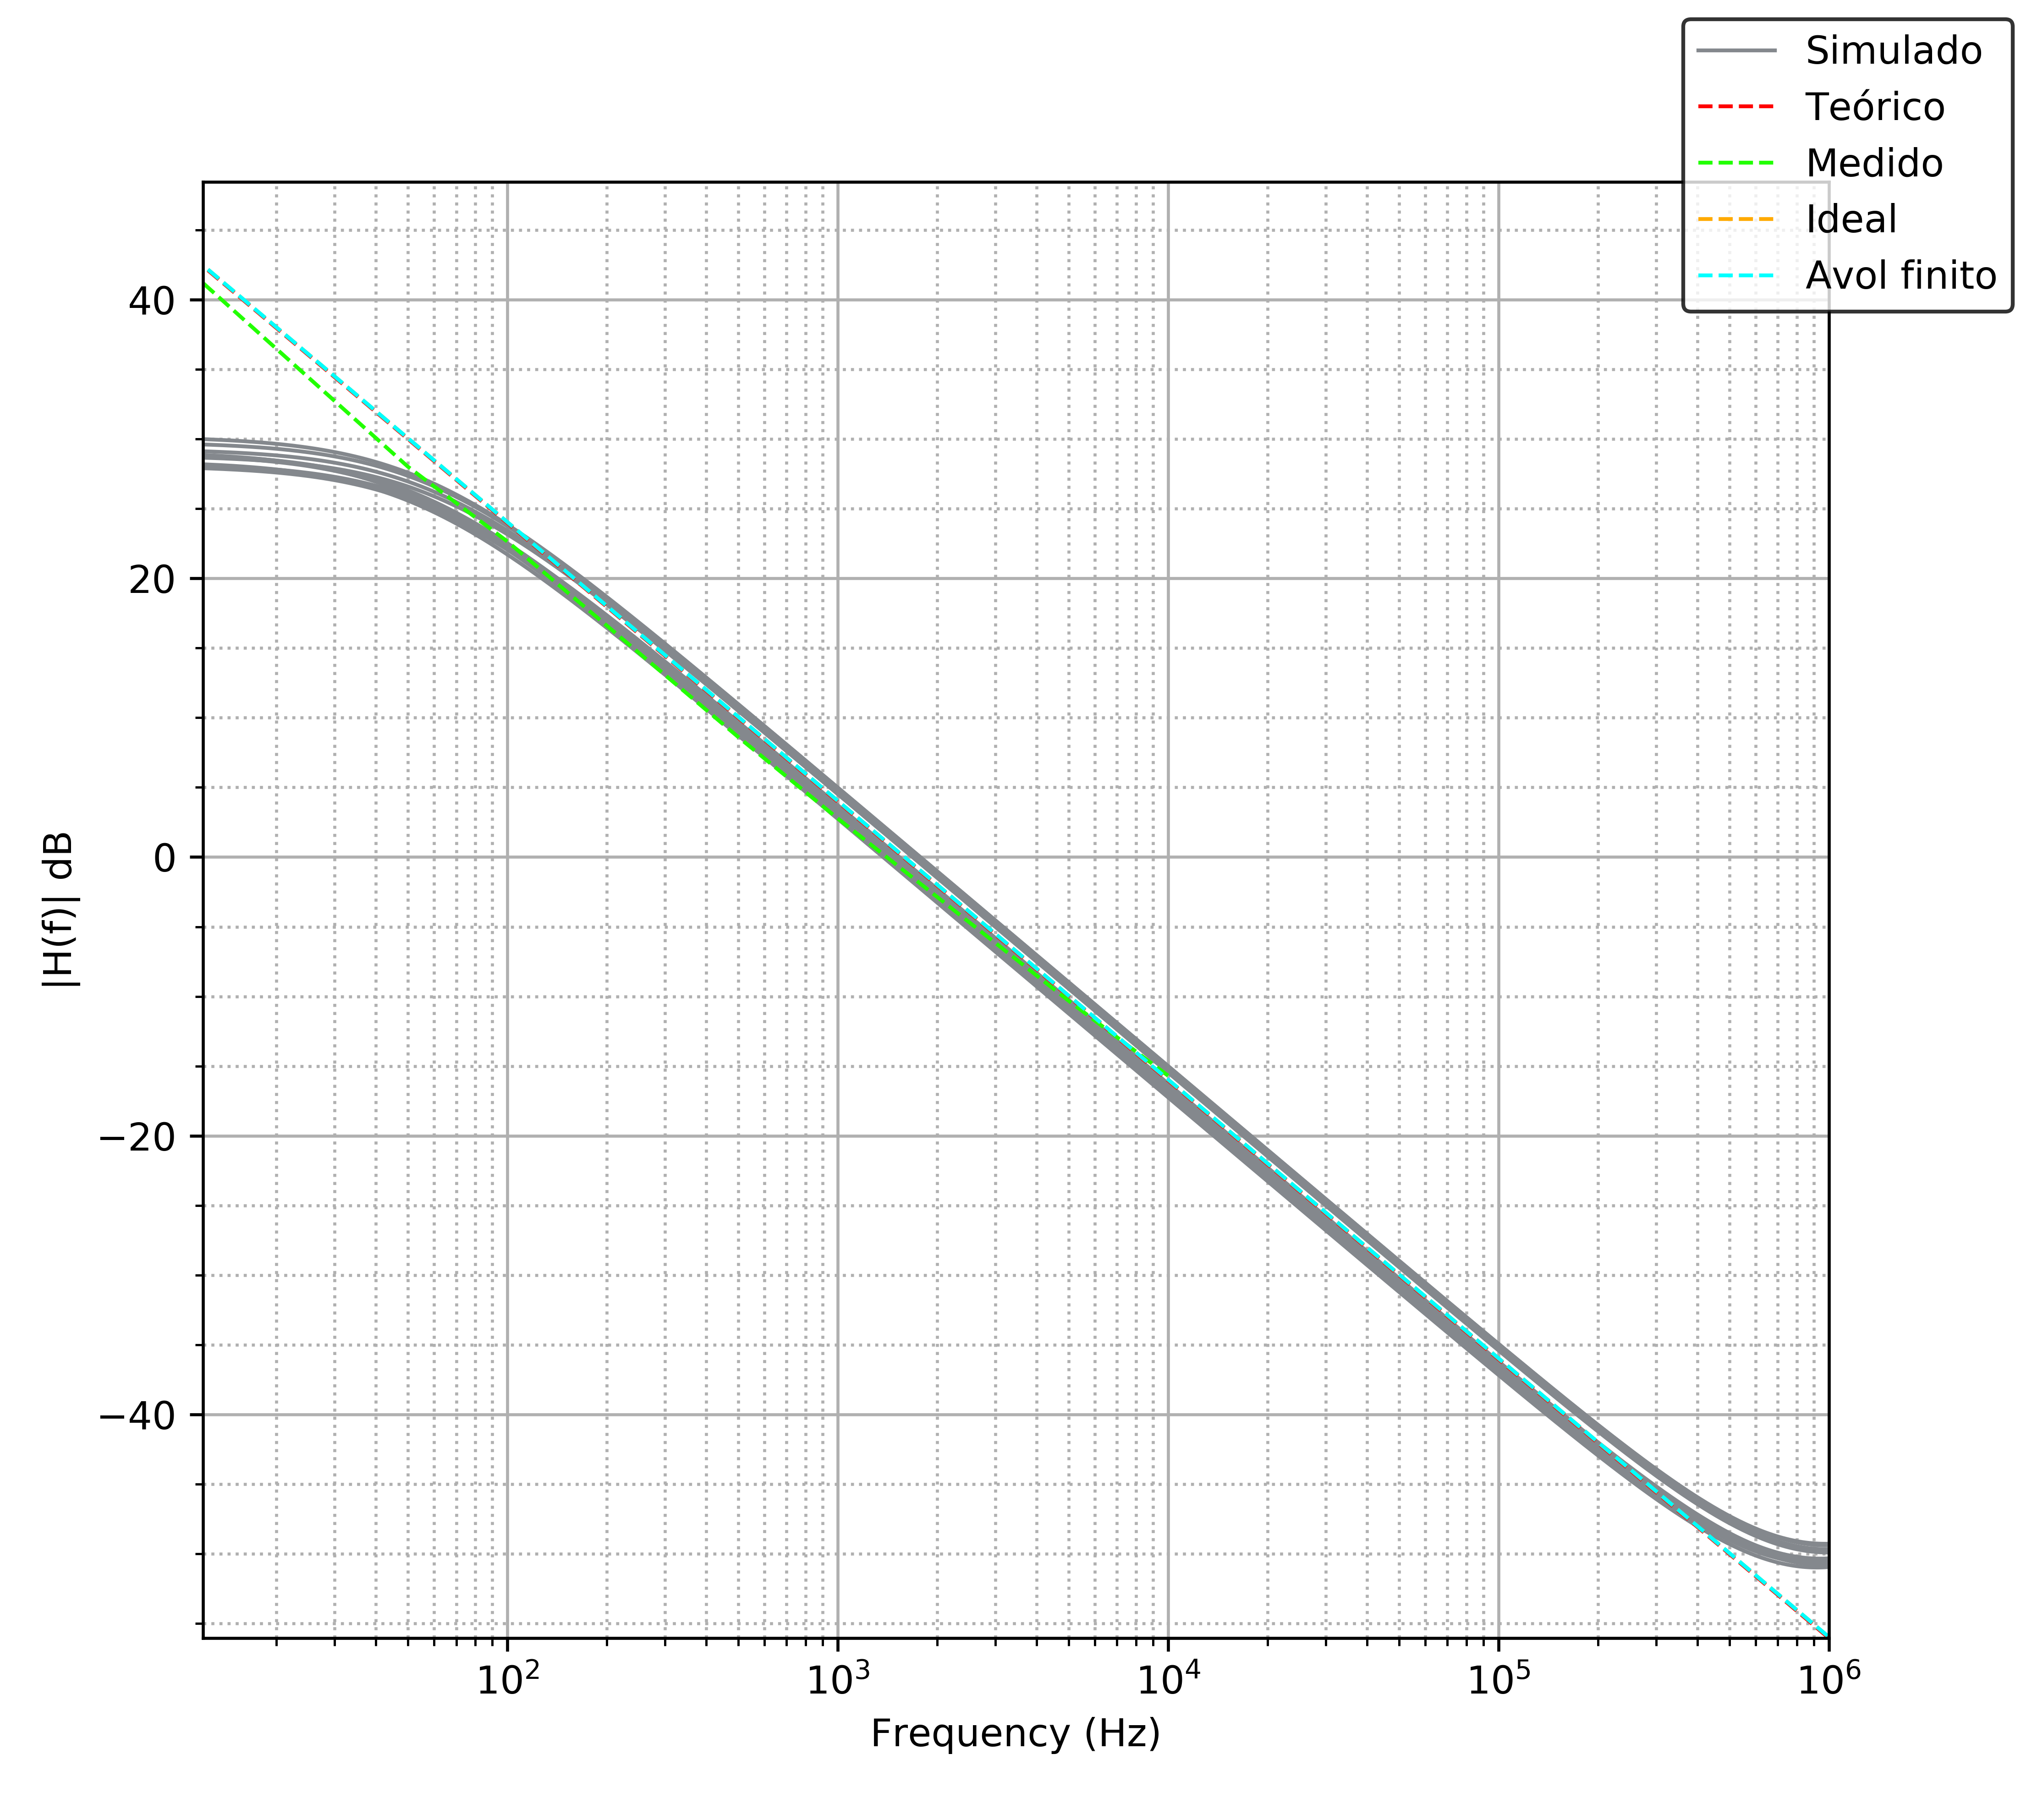
\includegraphics[scale=0.6]{Recursos/Integrador/bode_modulo.png}
	\caption{Diagrama de bode en m\'odulo del integrador sin compensar}
	\label{fig:integrador_bode_modulo}
\end{figure}

\begin{figure}[H]
	\centering
	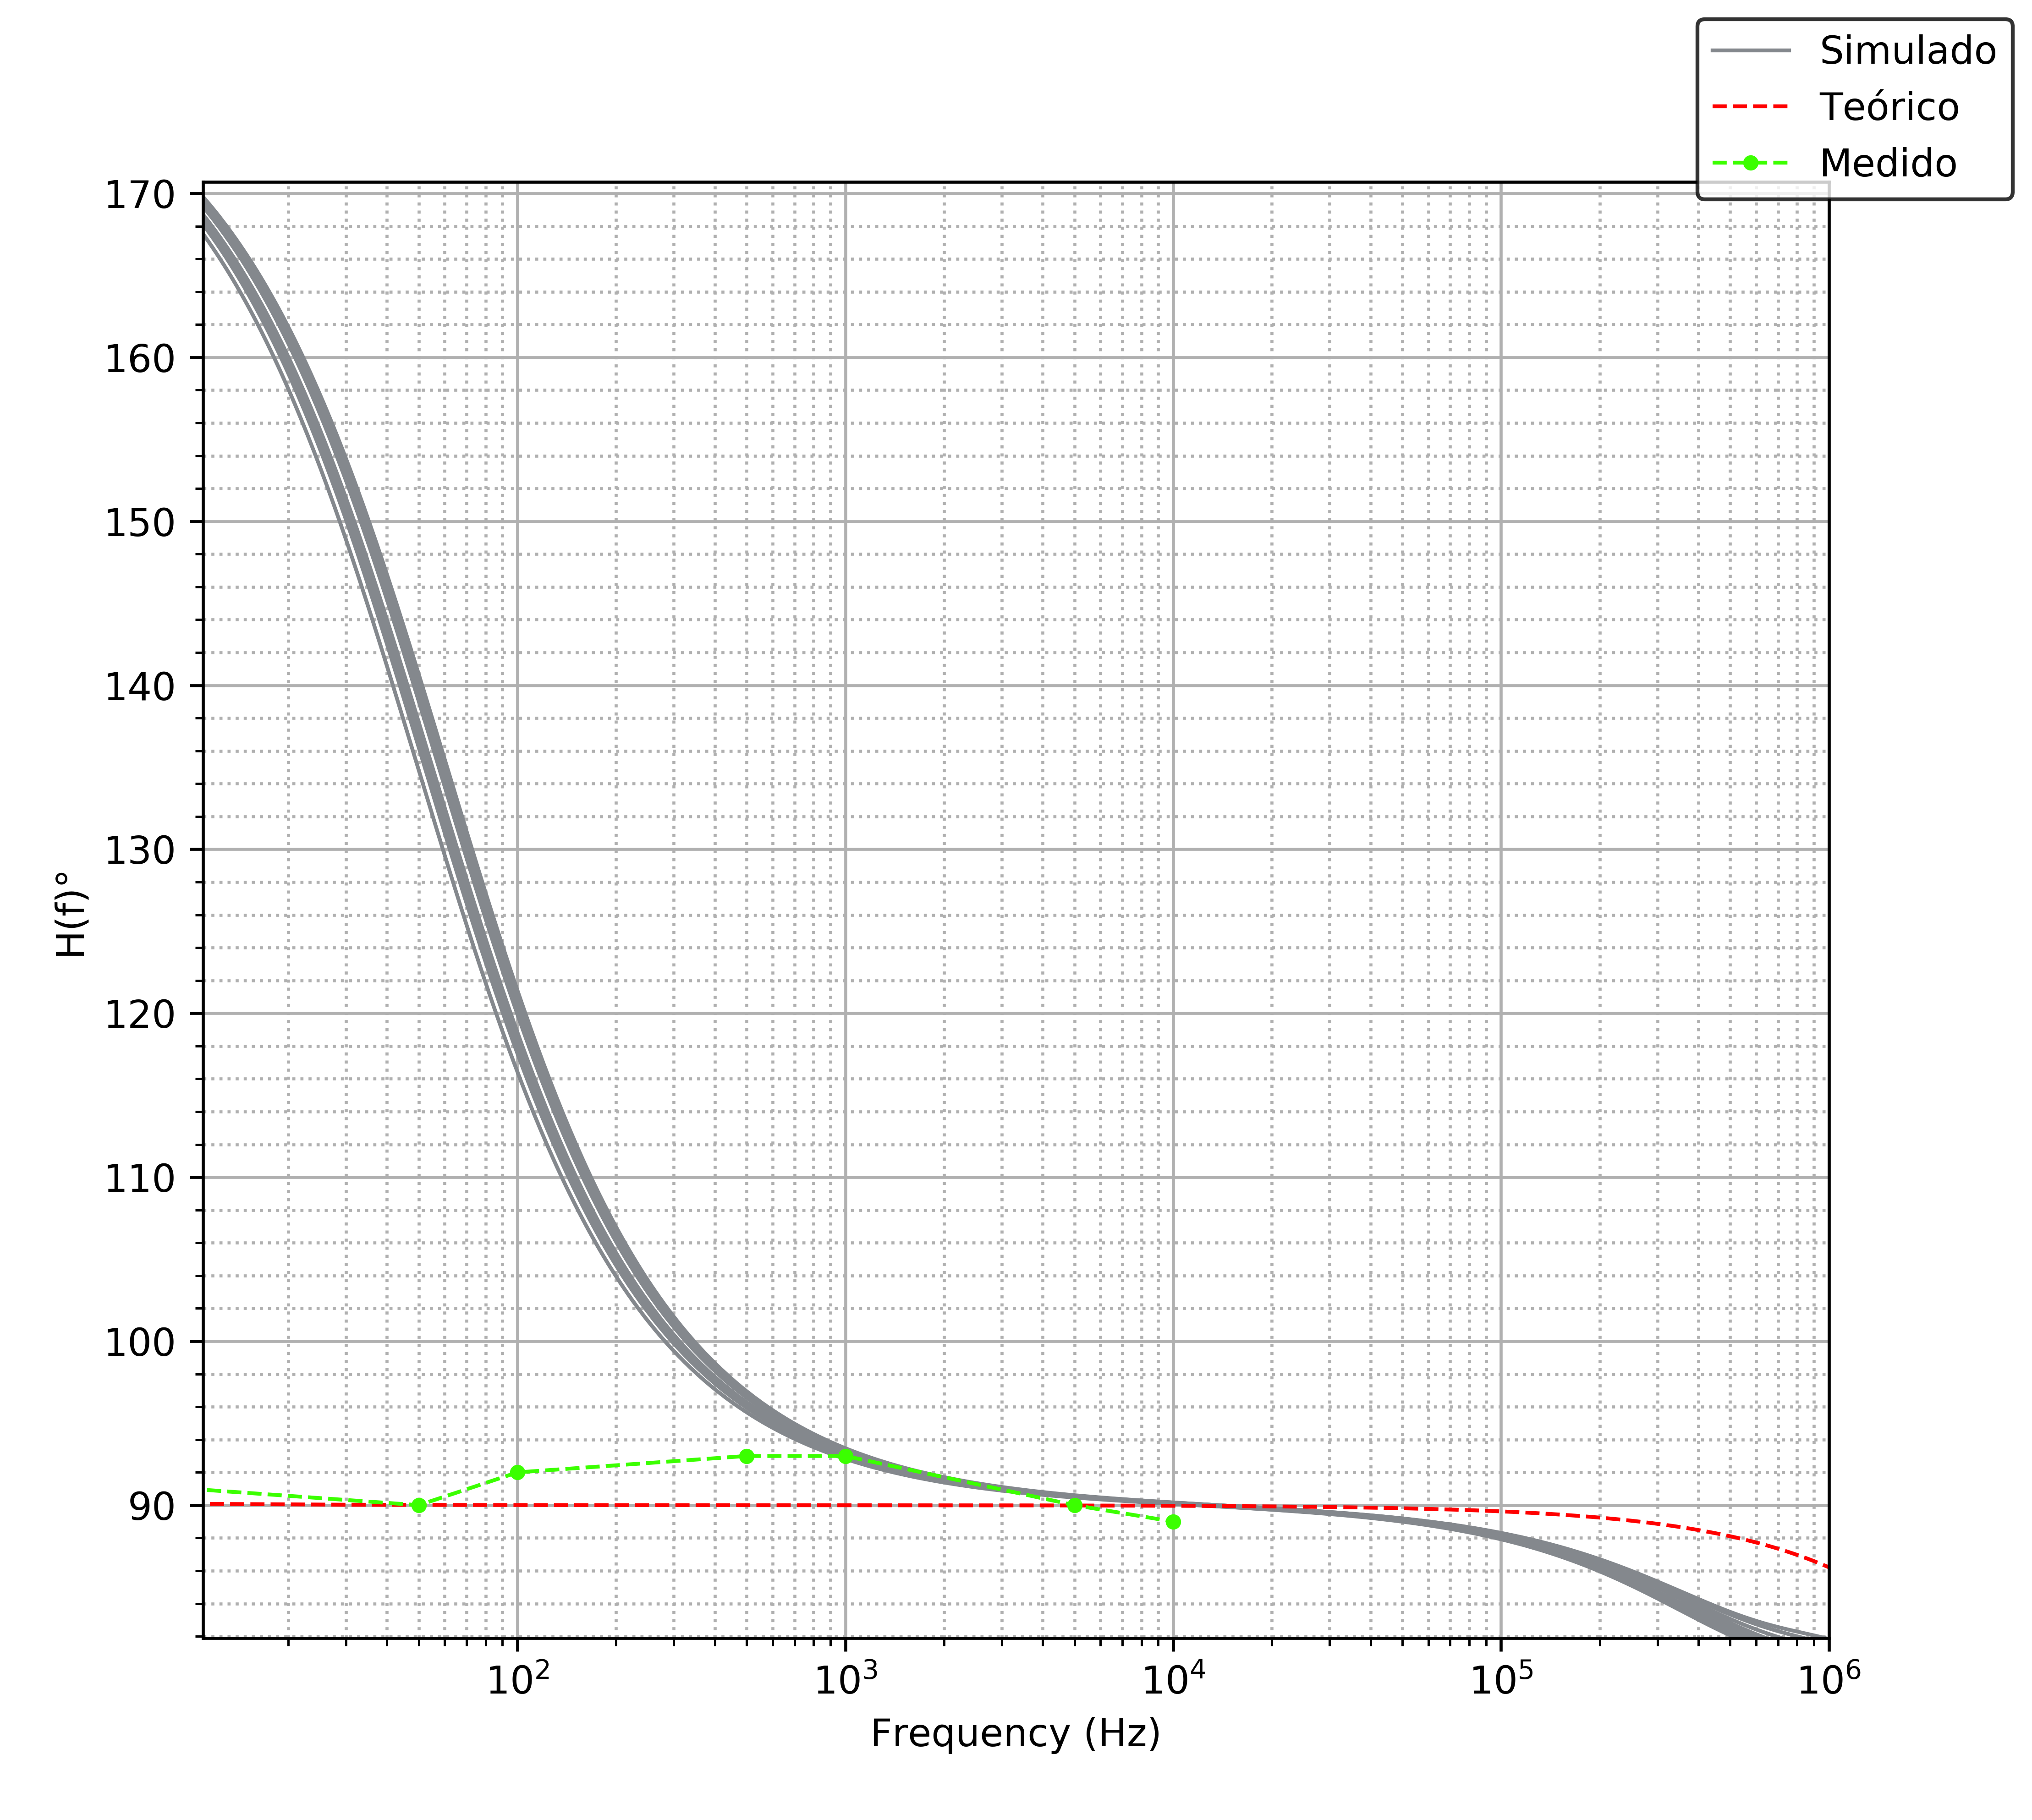
\includegraphics[scale=0.6]{Recursos/Integrador/bode_fase.png}
	\caption{Diagrama de bode en fase del integrador sin compensar}
	\label{fig:integrador_bode_fase}
\end{figure}

\paragraph*{Impedancia de entrada} en t\'erminos generales, tanto la respuesta en frecuencia como la impedancia de entrada
obtenidos en la medici\'on y en la simulaci\'on son resultados que en s\'i mismos no logran caracterizar al sistema correctamente por los efectos indeseados
de la saturaci\'on para bajas frecuencias del circuito. Esto \'ultimo tambi\'en se encuentra presente en LTSpice. En las figuras \ref{fig:integrador_simulacion} se puede observar
que seg\'un la frecuencia el nivel de continua se modifica por lo explicado anteriormente.

\begin{figure}[H]
	\centering
	\begin{tabular}{c c}
		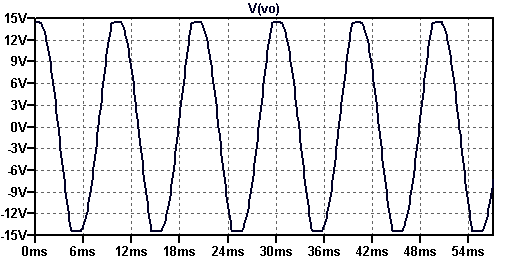
\includegraphics[scale=0.55]{Integrador/Simulaciones/Seno100.png} &
		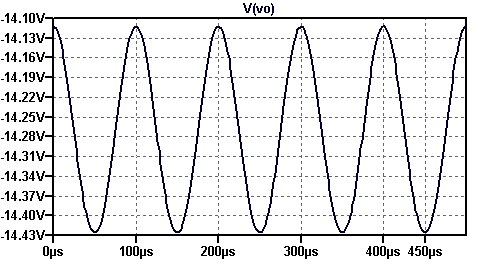
\includegraphics[scale=0.55]{Integrador/Simulaciones/Seno10k.png}
	\end{tabular}
	\caption{Respuesta del integrador sin compensar a senoidales de $100Hz$ y $10kHz$}
	\label{fig:integrador_simulacion}
\end{figure}

\begin{figure}[H]
	\centering
	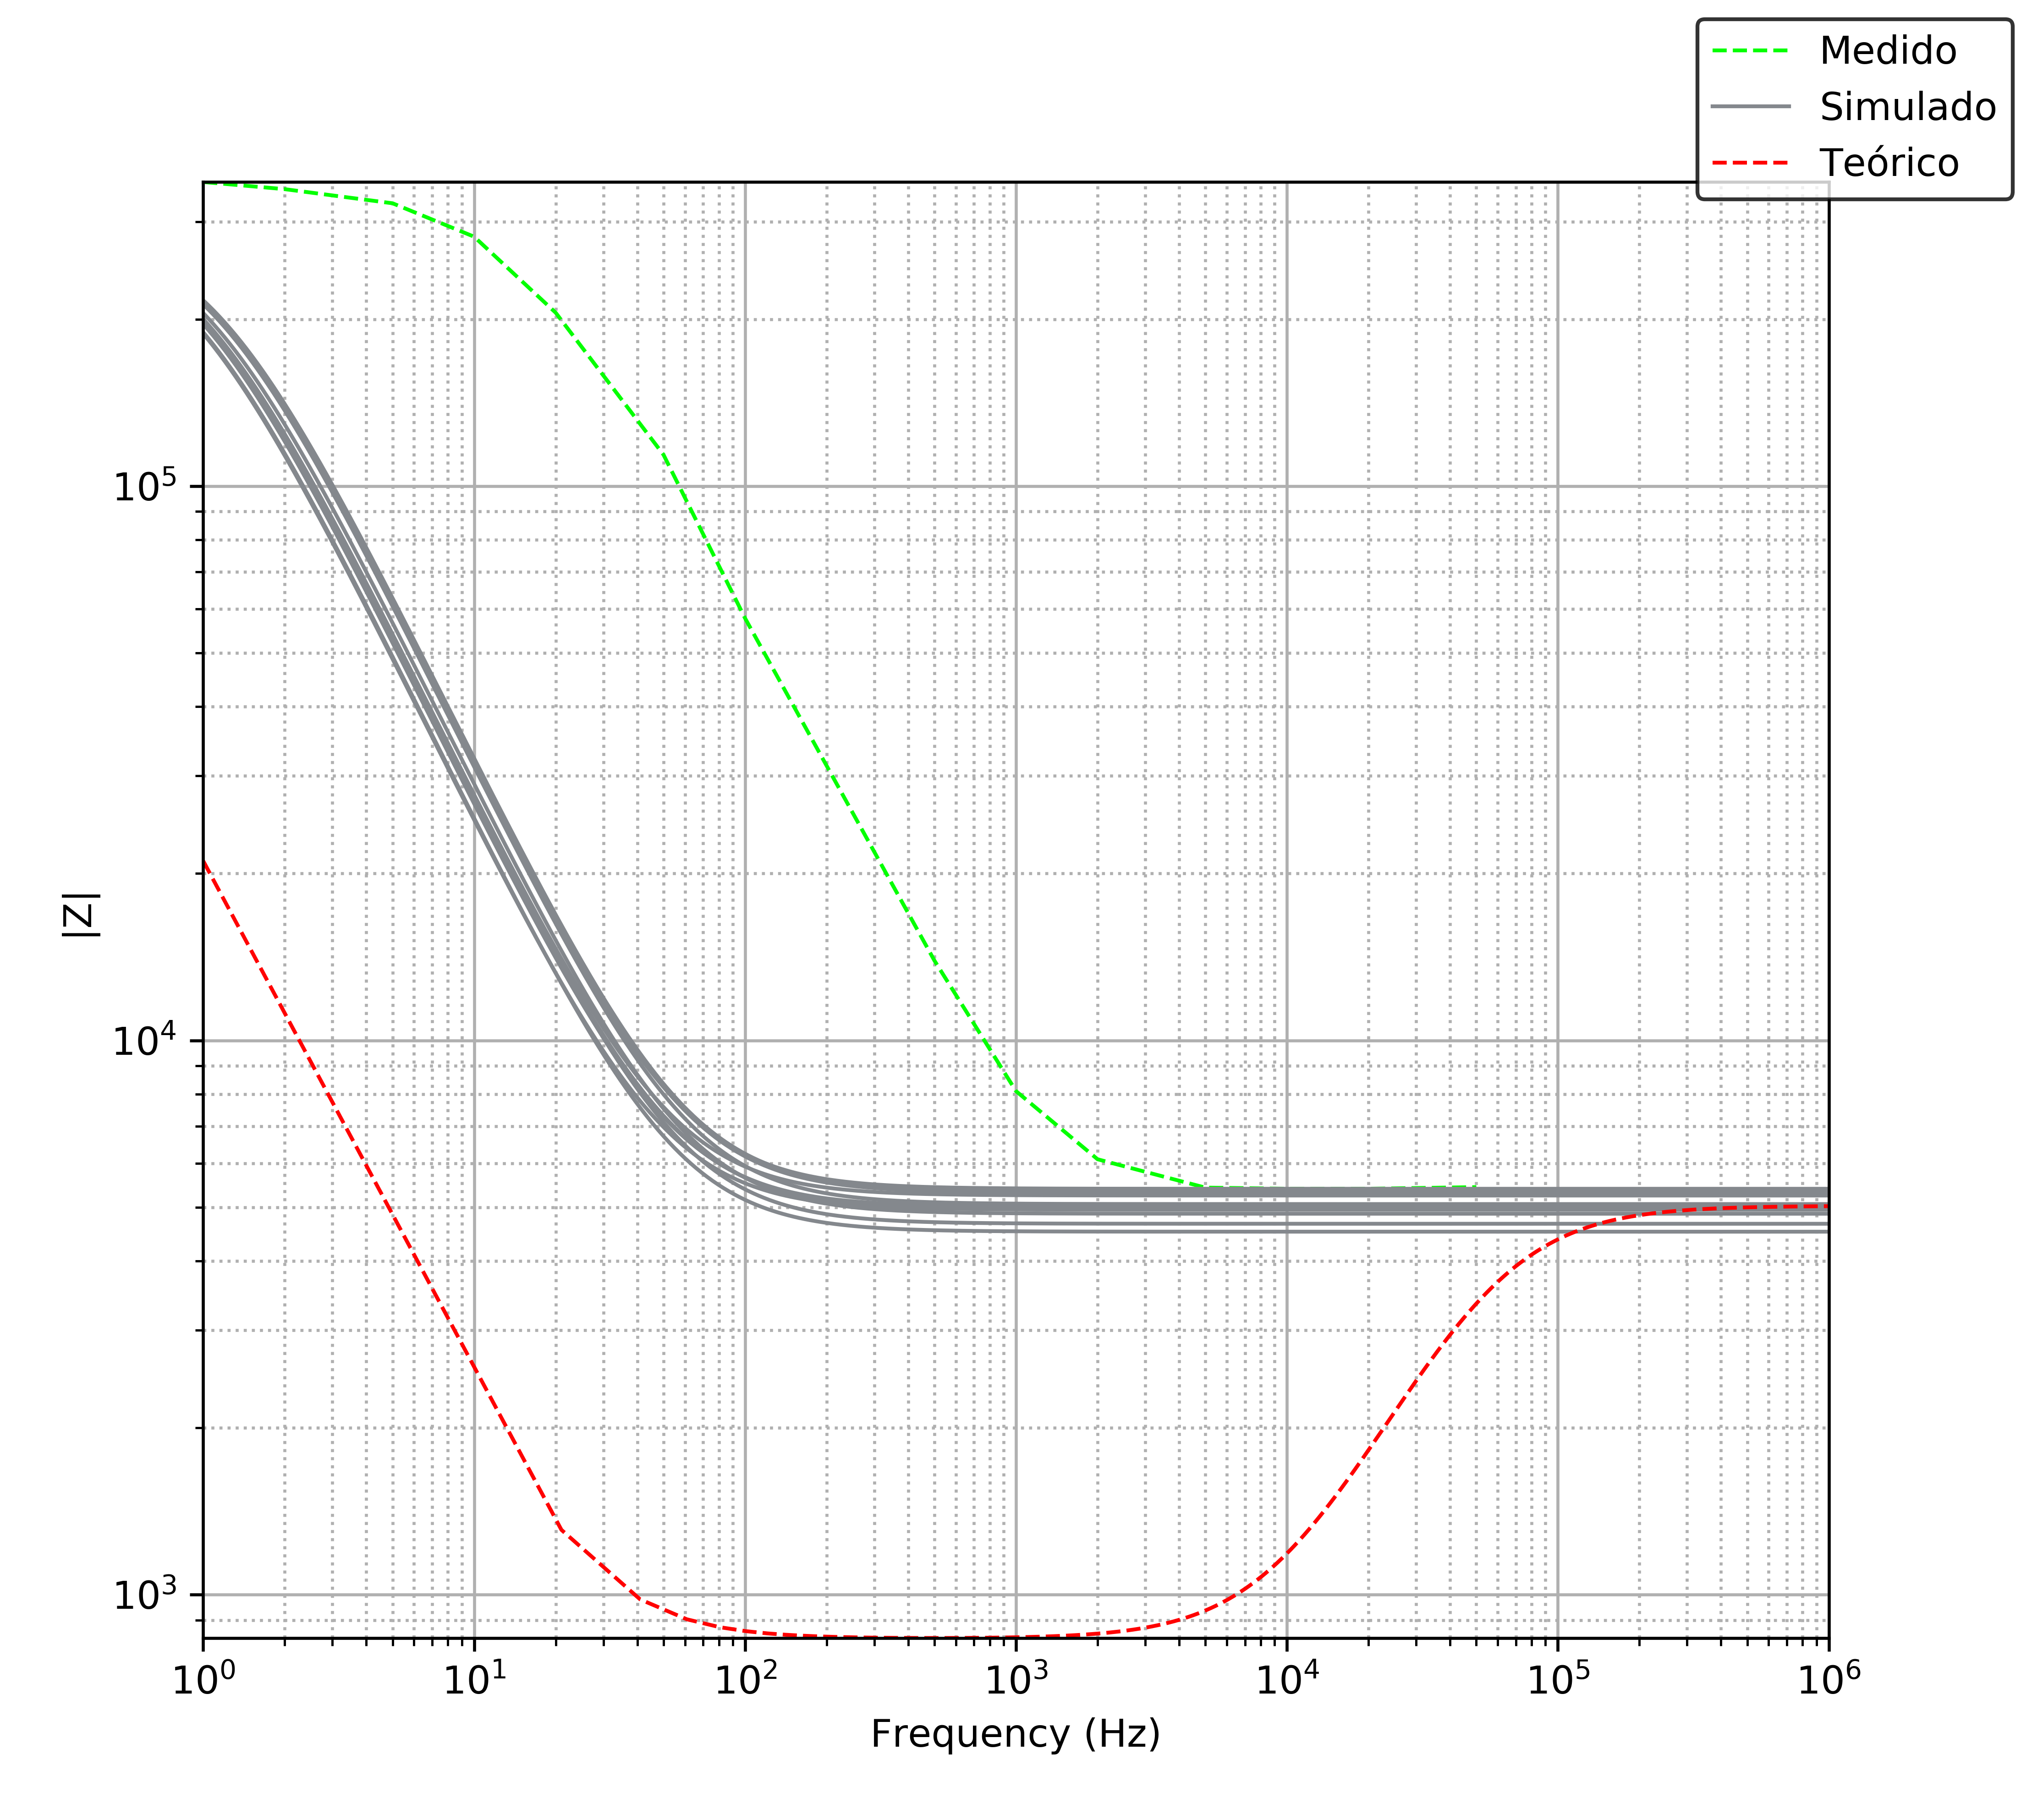
\includegraphics[scale=0.7]{Recursos/Integrador/impedancia_modulo.png}
	\caption{Impedancia de entrada en m\'odulo del integrador sin compensar}
	\label{fig:integrador_impedancia_modulo}
\end{figure}

\begin{figure}[H]
	\centering
	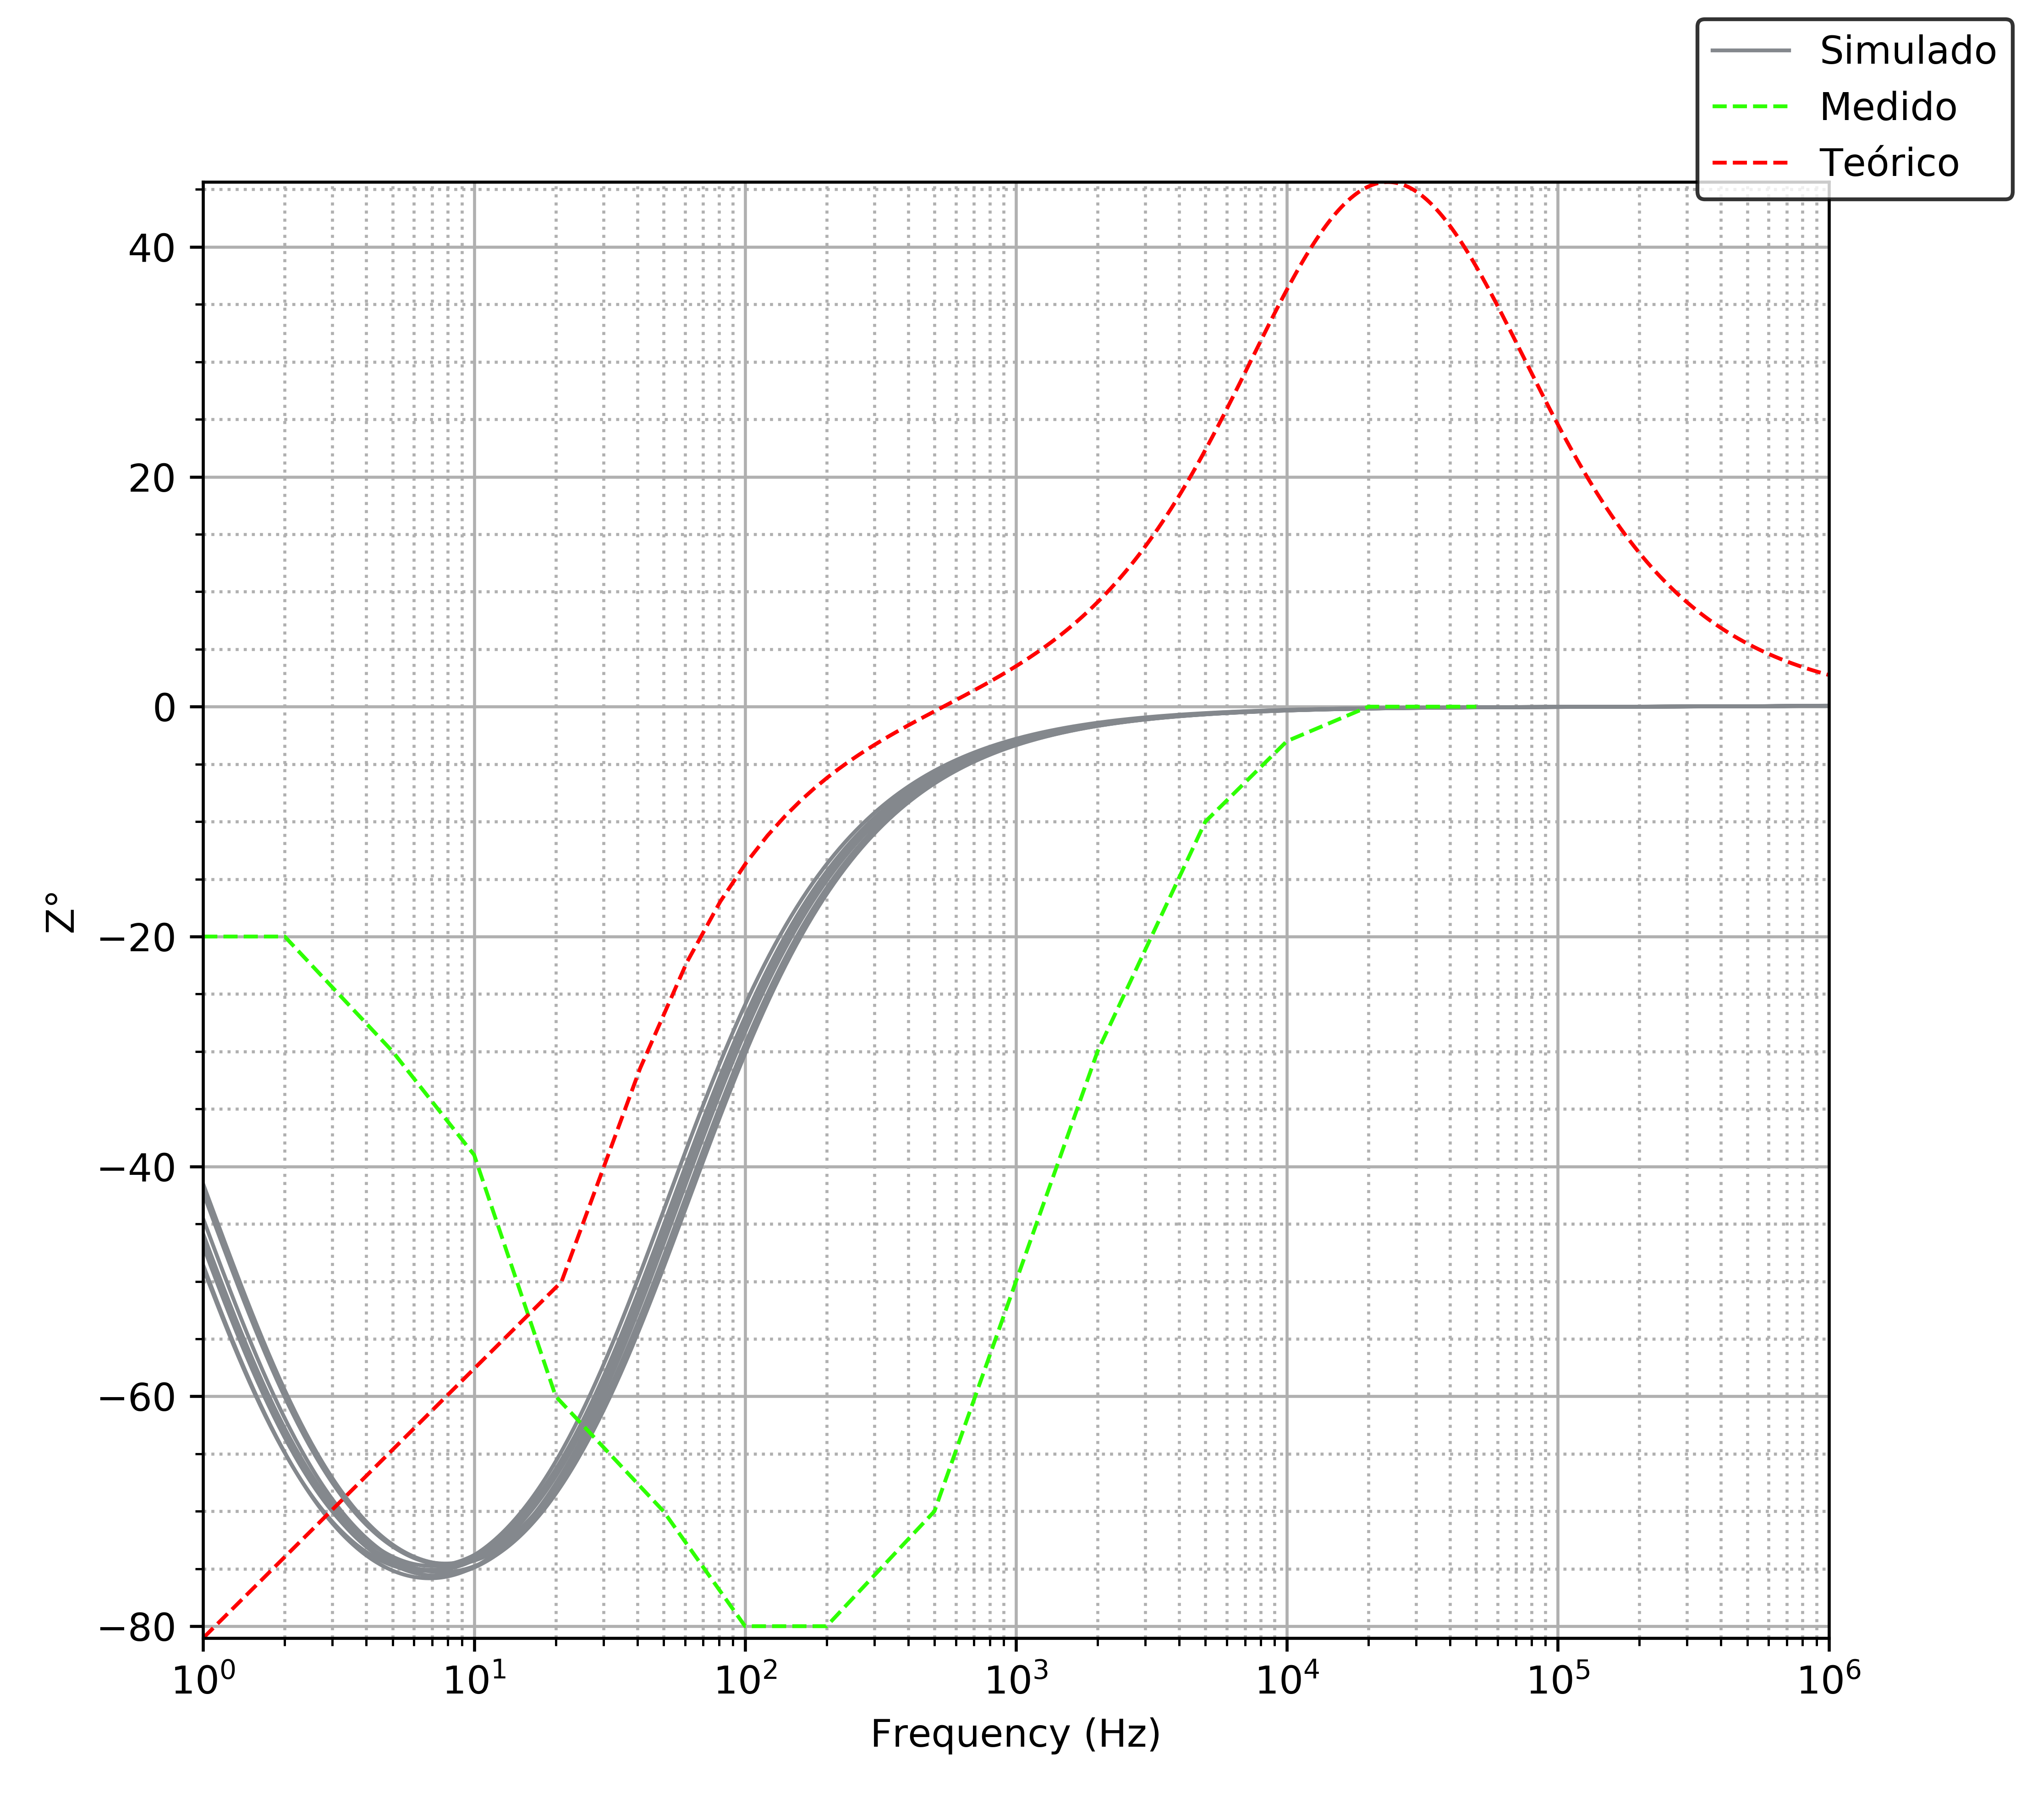
\includegraphics[scale=0.7]{Recursos/Integrador/impedancia_fase.png}
	\caption{Impedancia de entrada en fase del integrador sin compensar}
	\label{fig:integrador_impedancia_fase}
\end{figure}

\paragraph*{Respuesta a se\~nales no senoidales} A pesar de que se considera que el circuito como tal no funciona correctamente por el malfuncionamiento provocado ante las componetes de continuas,
se observ\'o la respuesta del circuito ante una se\~nal cuadrada y una se\~nal triangular, en ambos casos el resultado es en cierta forma apreciable, sin embargo se puede observar la presencia de continuas
seg\'un la frecuencia.

\begin{figure}[H]
	\centering
	\begin{tabular}{c c}
		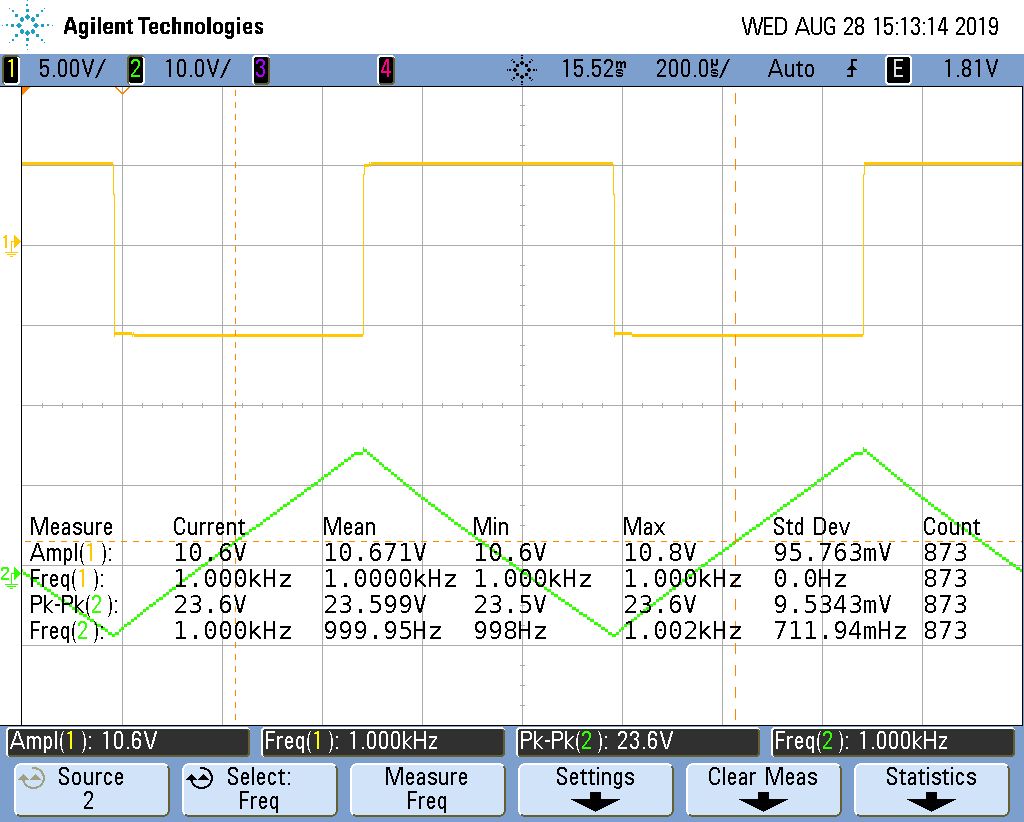
\includegraphics[scale=0.2]{Integrador/Mediciones/Osciloscopio/PCB_Sin_Compensar/osc_11.png} & 
		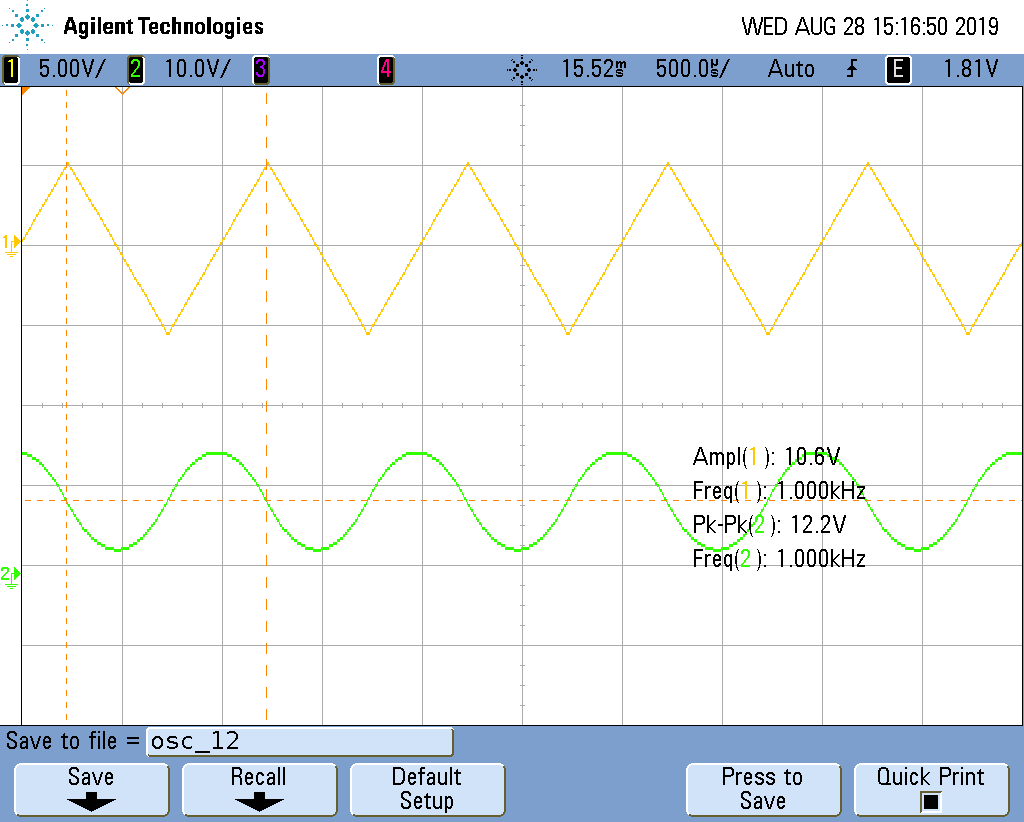
\includegraphics[scale=0.2]{Integrador/Mediciones/Osciloscopio/PCB_Sin_Compensar/osc_12.png}
	\end{tabular}
	\caption{Respuestas a se\~nales no senoidales}
	\label{fig:integrador_respuestas}
\end{figure}

	\subsection{Circuito integrador compensado}
A partir de los resultados de las mediciones y simulaciones del circuito integrador no compensado, se llega a la conclusi\'on de que como tal, el circuito no puede funcionar como integrador correctamente
y es necesario colocar una resistencia de compensaci\'on con el objetivo de limitar la ganancia para se\~nales de baja frecuencia. Por otro lado, se busca que el valor sea tal que el resultado no presente efectos no deseados como lo era para
el derivador un sobrepico por comportamientos subamortiguados, adem\'as de querer que el funcionamiento del integrador se d\'e en el mayor ancho de banda posible con un error en la fase menor a tres grados.

\subsubsection{An\'alisis Te\'orico}

\paragraph*{Funci\'on transferencia en condiciones ideales} utilizando la expresi\'on del amplificador inversor bajo condiciones ideales, se llama $Z_2$ a la impedancia que resulta del paralelo de la resistencia y el capacitor. Luego se obtiene:

\begin{equation*}
	Z_2 = R_2 // \frac{1}{s \cdot C} = \frac{R_2}{1 + s \cdot C \cdot R_2}
\end{equation*}

\begin{equation}
	H(s) = \frac{V_o(s)}{V_i(s)} = - \frac{Z_2}{R_1} = - \frac{\frac{R_2}{R_1}}{1 + s \cdot C \cdot R_2}
	\label{eq:integrador_compensado_transfer_ideal}
\end{equation}

\paragraph*{Funci\'on transferencia con $A_{vol}$ finito} considerando la misma impedancia del paralelo en la realimentaci\'on que en la resoluci\'on ideal, se calcula el valor del potencial en la pata inversora del amplificador operacional y luego se halla la expresi\'on de la funci\'on de la siguiente manera:

\begin{equation*}
	v^{-} = V_o \cdot \frac{R_1}{R_1+ Z_2} + V_i \cdot \frac{Z_2}{Z_2 + R_1} \Rightarrow
	v^{-} = \frac{V_o \cdot R_1 \cdot ( 1 + s \cdot C \cdot R_2) + V_i \cdot R_2}{R_2 + R_1 \cdot (1 + s \cdot C \cdot R_2)}
\end{equation*}

\begin{align*}
	V_o = (v^{+} - v^{-}) \cdot A_{vol} = - A_{vol} \cdot \frac{V_o \cdot R_1 \cdot ( 1 + s \cdot C \cdot R_2) + R_2 \cdot V_i}{R_1 + R_2 + s \cdot C \cdot R_1 \cdot R_2} \Rightarrow \\
	V_o \cdot \left[ 1 + \frac{A_{vol} \cdot R_1 \cdot ( 1 + s \cdot C \cdot R_2)}{R_1 + R_2 + s \cdot C \cdot R_1 \cdot R_2} \right] =
	V_i \cdot \frac{-A_{vol} \cdot R_2}{R_1 + R_2 + s \cdot C \cdot R_1 \cdot R_2} 
\end{align*}

\begin{equation}
	H(s) = \frac{- A_{vol} \cdot R_2}{R_1 \cdot ( 1 + A_{vol} ) + R_2} \cdot \frac{1}{1 + s \cdot \frac{C \cdot R_1 \cdot R_2 \cdot ( 1 + A_{vol})}{R_1 \cdot (1 + A_{vol}) + R_2}}
	\label{eq:integrador_compensado_transfer_avol_finito}
\end{equation}

\paragraph*{Funci\'on transferencia con polo dominante} luego reemplazando en la expresi\'on anterior la forma del $A_{vol}(\omega)$ se obtiene:

\begin{equation*}
	H(s) = \frac{-A_o \cdot \omega_p \cdot R_2}{R_1 \cdot ( A_o \cdot \omega_p + s + \omega_p) + R_2 \cdot (s + \omega_p)} \cdot \frac{1}{1 + s \cdot \frac{C \cdot R_1 \cdot R_2 \cdot ( A_o \cdot \omega_p + s + \omega_p)}{R_2 \cdot ( s + \omega_p) + R_1 \cdot (A_o \cdot \omega_p + s + \omega_p)}}
\end{equation*}

\begin{equation}
	H(s) = \frac{-A_o \cdot R_2}{R_2 + R_1 \cdot (1+A_o)} \cdot \frac{1}{1 + s \cdot \frac{C \cdot R_1 \cdot R_2 \cdot \omega_p \cdot (A_o + 1) + R_1 + R_2}{\omega_p \cdot (R_2 + R_1 \cdot(A_o + 1))} + s^{2} \cdot \frac{C \cdot R_1 \cdot R_2}{\omega_p \cdot (R_2 + R_1 \cdot (A_o + 1))}}
	\label{eq:integrador_compensado_transfer_polo_dominante}
\end{equation}

\paragraph*{Impedancia de entrada con $A_{vol}$ finito} llamando como $Z_2$ al paralelo entre la resistencia y el capacitor en el lazo de la realimentaci\'on y luego aplicando ley de nodos, se obtiene:

\begin{align*}
	I_1 & = I_2 + I_3 \Rightarrow \frac{V_i + V_d}{R_1} = \frac{-V_d}{R_{id}} + \frac{-V_d - V_d \cdot A_{vol}}{Z_o + Z_2}\\
	& \Rightarrow
	V_d = \frac{- V_i \cdot r_{id} \cdot \left[ R_2 + Z_o \cdot (1 + s \cdot C \cdot R_2) \right]}{(R_1 + r_{id}) \cdot \left[R_2 + Z_o \cdot (1 + s \cdot C \cdot R_2) \right] + (1 + A_{vol}) \cdot ( 1 + s \cdot C \cdot R_2) \cdot R_1 \cdot r_{id}}
\end{align*}

\begin{align}
	Z_{in}(s) = \frac{V_i}{I_1} = \frac{(R_1 + r_{id}) \cdot (R_2 + Z_o) + (1 + A_{vol}) \cdot (R_1 + r_{id})}{R_2 + Z_o + r_{id} \cdot(1 + A_{vol})} \cdot \frac{1 + s \cdot \frac{C \cdot R_2 \cdot \left[ Z_o \cdot (R_1 + r_{id}) + R_1 \cdot r_{id} \cdot ( 1 + A_{vol}) \right]}{(R_1 + r_{id}) \cdot (R_2 + Z_o) + (1 + A_{vol}) \cdot R_1 \cdot r_{id}}}{1 + s \cdot \frac{C \cdot R_2 \left[ Z_o + r_{id} \cdot ( 1 + A_{vol}) \right]}{R_2 + Z_o + r_{id} \cdot ( 1 + A_{vol})}}
\end{align}

\paragraph*{Impedancia de entrada con polo dominante} reemplazando $A_{vol}$ por su expresi\'on incluyendo el polo dominante, se llega luego de unos pasos algebraicos a que:

\begin{align}
	Z_{in}(s) = \frac{(R_1+r_{id})\cdot(R_2 + Z_o) + R_1 \cdot r_{id} \cdot(1+A_o)}{R_2 + Z_o + r_{id} \cdot(1 + A_o)} \cdot \frac{1 + s \cdot \beta + s^{2} \cdot \alpha}{1 + s \cdot b + s^{2} \cdot a }
\end{align}

\begin{align*}
	a & = \frac{C \cdot R_2 \cdot (Z_o + r_{id})}{\omega_p \cdot \left[ R_2 + Z_o + r_{id} \cdot(1 + A_o) \right]} \\
	b & = \frac{R_2 + Z_o + r_{id} + \omega_p \cdot C \cdot R_2 \cdot \left[ Z_o + (1 + A_o) \cdot r_{id} \right] }{\omega_p \cdot \left[ R_2 + Z_o + r_{id} \cdot(1 + A_o) \right] } \\
	\alpha & = \frac{C \cdot R_2 \cdot \left[ (R_1 + r_{id}) \cdot Z_o + R_1 \cdot r_{id} \right] }{\omega_p \left[ (R_1 + r_{id}) \cdot (R_2 + Z_o) + R_1 \cdot r_{id} \cdot(1 + A_o) \right]} \\
	\beta & = \frac{(R_1 + r_{id}) \cdot \left[C \cdot R_2 \cdot Z_o \cdot \omega_p + R_2 + Z_o \right] + R_1 \cdot r_{id} \cdot \left[ 1 + C \cdot R_2 \cdot \omega_p \cdot (A_o + 1) \right] }{\omega_p \left[ (R_1 + r_{id}) \cdot (R_2 + Z_o) + R_1 \cdot r_{id} \cdot(1 + A_o) \right] }
\end{align*}

\paragraph*{Expresiones finales} para finalizar con el dise\~no y an\'alisis te\'orico del integrador compensado es necesario determinar el valor de la resistencia de compensaci\'on que debe ser colocada en paralelo
al capacitor, para que de esta forma se logre que en bajas frecuencias cuando el lazo de realimentaci\'on por el capacitor se ve debilitado, la resistencia mantenga tal realimentaci\'on. Por otro lado, a dicha resistencia se le imponen
las condiciones mencionadas al principio de esta secci\'on, estas son, que no presente sobrepicos la respuesta en frecuencia, que integre en el mayor rango de frecuencias con un error de fase menor a 3 grados y se logre compensar
efectivamente el circuito.

Para lograr estas condiciones, se propone an\'alizar te\'oricamente cu\'ales son las componentes de corriente continua del $LM833$ que pueden provocar la saturaci\'on
del integrador incluso cuando no hay entrada. Para ello se analiza el efecto de las corrientes de bias y la tensi\'on de polarizaci\'on del amplificador operacional.
Analizando la hoja de datos, se obtiene que la corriente de bias tiene un valor de $I_{io} = 200nA$ y la tensi\'on de polarizaci\'on es de
$V_{io} = 5mV$. Utilizando esto para limitar el valor de tensi\'on de salida de forma que no haya saturaci\'on y considerando que el circuito se encuentra configurado
de forma \'optima para el menor efecto de las corrientes de bias, se encuentra que la componente de salida de continua y sobre ella se imponen tales restricciones, considerando que en el peor caso se quiere una tensi\'on de salida m\'axima de $V_{max} = 1V$ simplemente 
para tener un valor de resistencia de referencia que no se puede sobrepasar
, y luego imponiendo como una condici\'on adicional, que la frecuencia de corte como m\'axmio debe estar ubicada en aproximadamente $f_o = 20Hz$ para
 lograr un ancho de banda amplio dentro del cual se integre correctamente, se llega a que:

\begin{equation*}
	V_{dc} = (200nA) \cdot R_2 + 5mV \cdot ( 1 + \frac{R_2}{R_1} )
	\Rightarrow
	R_2 < 829,16 k \Omega 
\end{equation*}

\begin{align*}
	f_o & = \frac{1}{2 \pi \cdot C \cdot R_2} 
	\Rightarrow
	R_2 > \frac{1}{2 \pi \cdot C \cdot f_o}
	\Rightarrow
	R_2 > 397,89k \Omega
\end{align*}

En consecuencia se opta por tomar un valor de resistencia $R_2 = 470k\Omega$ puesto que ajusta correctamente en el rango de los criterios adoptados.

\begin{equation}
	H(s) = \frac{-93,91}{1 + s \cdot 9,392 \cdot 10^{-3} + \left( \frac{s}{2 \pi \cdot 15,94kHz} \right)^{2}}
\end{equation}

=======

\begin{equation}
	H(s) = - \frac{\frac{1}{s \cdot C}}{R} = - \frac{1}{s \cdot C \cdot R}
	\Rightarrow
	H(s) = - \frac{1}{\frac{s}{2 \pi \cdot 1,591kHz}}
	\label{eq:integrador_transfer_ideal}
\end{equation}

En este primer acercamiento al comportamiento del circuito, se puede observar en la funci\'on transferencia que se describe un sistema que no es bibo-estable como se asumi\'o en un principio, sino que posee un polo en el origen. Esto \'ultimo tiene sentido porque implica que para entradas acotadas, la respuesta ser\'a la integral de dicha entrada acotada, pudiendo dar un resultado no acotado en el tiempo. Desde otro punto de vista, para frecuencias muy bajas o se\~nales continuas, la impedancia del capacitor en la realimentaci\'on es demasiado grande y provoca una desconexi\'on o un lazo d\'ebil, por lo tanto el amplificador operacional satura puesto que amplifica en t\'erminos de su $A_{vol}$ correspondiente seg\'un sea el caso.

\paragraph*{Funci\'on transferencia con $A_{vol}$ finito} consid\'erese un $A_{vol}$ finito, luego se plantean los valores de potencial el\'ectrico sobre los terminales de las entradas del amplificador operacional y se calcula la salida con la ecuaci\'on correspondiente al modelo del mismo. Entonces, se obtiene:

\begin{equation*}
	v^{-} = V_i \cdot \frac{\frac{1}{s \cdot C}}{\frac{1}{s \cdot C} + R} + V_o \cdot \frac{R}{\frac{1}{s \cdot C} + R}
	\Rightarrow
	v^{-} = \frac{V_i + V_o \cdot s \cdot C \cdot R}{1 + s \cdot C \cdot R}
\end{equation*}

\begin{equation*}
	V_o = (v^{+} - v^{-}) \cdot A_{vol} \Rightarrow
	V_o \cdot \left[ 1 + \frac{A_{vol} \cdot s \cdot R \cdot C}{1 + s \cdot C \cdot R} \right] =
	- V_i \cdot \frac{A_{vol}}{1 + s \cdot C \cdot R}
\end{equation*}

\begin{equation}
	H(s) = \frac{V_o(s)}{V_i(s)} = \frac{-A_{vol}}{1 + s \cdot C \cdot R \cdot (A_{vol} + 1)}
	\Rightarrow
	H(s) = \frac{-100000}{1 + \frac{s}{2 \pi \cdot 0,0159Hz}}
	\label{eq:integrador_transfer_avol_finito}
\end{equation}

Se puede observar que con estas nuevas consideraciones, el sistema dej\'o de ser inestable en t\'erminos de su respuesta, no obstante sigue sucediendo que para frecuencias muy bajas la realimentaci\'on pasa a tener un lazo d\'ebil y satura el amplificador operacional.

\paragraph*{Funci\'on transferencia con polo dominante} ahora se considera que la ganancia del amplificador operacional tiene el polo dominante, con lo cual no se mantiene invariante en frecuencia. Reutilizando la expresi\'on anterior para $A_{vol}$ finito y reemplazando tal t\'ermino por la expresi\'on con el polo dominante se obtiene:

\begin{equation*}
	H(s) = - \frac{A_o \cdot \omega_p}{s + \omega_p + s \cdot C \cdot R \cdot (A_o \cdot \omega_p + s + \omega_p)}
	\Rightarrow
	H(s) = - \frac{A_o}{1 + s \cdot \frac{1 + C \cdot R \cdot \omega_p \cdot ( A_o + 1 )}{\omega_p} + s^{2} \cdot \frac{C \cdot R}{\omega_p}}
\end{equation*}

\begin{equation*}
	H(s) = - \frac{100000}{1 + s \cdot 10,001 + \left( \frac{s}{2 \pi \cdot 488,60Hz} \right)^{2}}
\end{equation*}

En esta nueva expresi\'on de la funci\'on transferencia, el sistema refleja un segundo orden en el denominador del cual se pueden determinar los par\'ametros caracter\'isticos del mismo, obteniendo que $\omega_o = 3069,96 \frac{1}{s}$ y $\xi = 15351,58 \geq 1$. Entonces el sistema se encuentra en un sobreamortiguamiento con frecuencias de corte ubicadas en $f_1 = 15,0017MHz$ y $f_2 = 0,01499Hz$.

\begin{equation}
	H(s) = - \frac{106092,66}{(1 + \frac{s}{2 \pi \cdot 0,014998Hz}) \cdot (1 + \frac{s}{2 \pi \cdot 15,0017MHz})}
	\label{eq:integrador_transfer_polo_dominante}
\end{equation}

En este nuevo resultado la \'unica diferencia con respecto al anterior, es que ahora hay un polo adicional que aparece en una frecuencia muy alejada, no obstante sigue saturando para frecuencias muy bajas por el lazo d\'ebil, es por esto que este circuito no funcionar\'a correctamente con el prop\'osito para el que fue pensado desde un punto de vista ideal, por ende ser\'a necesario realizar alguna compensaci\'on para poder corregirlo.

\paragraph*{Impedancia de entrada con $A_{vol}$ finito} para encontrar la impedancia de entrada considerando el $A_{vol}$ finito, se redibuja el circuito reemplazando al amplificador operacional con su circuito equivalente y se plantea la ley de nodos.
Se llama a la diferencia de potencial $V_d = V^{+} - V^{-}$.

\begin{figure}[H]
	\centering
	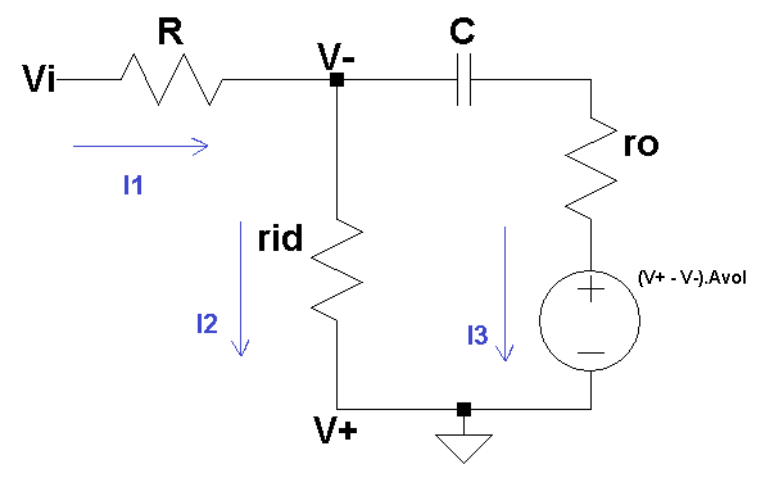
\includegraphics[scale=0.7]{Recursos/Integrador/Circuito_integrador_modelo_impedancia.png}
	\caption{Circuito equivalente para c\'alculo de impedancia de entrada}
	\label{fig:integrador_modelo}
\end{figure}

\begin{equation*}
	I_1 = I_2 + I_3 \Rightarrow
	\frac{V_i + V_d}{R_1} = 
	\frac{-V_i}{R_1} + \frac{- V_i - V_i \cdot A_{vol}}{\frac{1}{s \cdot C} + R}
\end{equation*}

\begin{equation*}
	V_d = \frac{- V_i \cdot r_i \cdot ( 1 + s \cdot C \cdot Z_o)}{r_i \cdot(s \cdot C \cdot Z_o + 1) + R_1 \cdot (1 + s \cdot C \cdot Z_o) + s \cdot C \cdot R_1 \cdot r_i \cdot (1 + A_{vol})}
\end{equation*}

\begin{equation*}
	Z_i(s) = \frac{V_i(s)}{I_1(s)} = \frac{V_i(s)}{\frac{V_i(s) + V_d(s)}{R_1}}
	\Rightarrow
	Z_i(s) = (R_1 + r_i) \cdot \frac{1 + s \cdot \frac{C \cdot \left[ Z_o \cdot (R_1 + r_i) + R_1 \cdot r_i \cdot (A_{vol} + 1) \right]}{R_1 + r_i}}{1 + s \cdot C \left[ Z_o + r_i \cdot ( 1 + A_{vol}) \right]}
\end{equation*}

\begin{equation}
	Z_i(s) = (180k \Omega) \cdot \frac{1 + \frac{s}{2 \pi \cdot 0,0163Hz}}{1 + \frac{s}{2 \pi \cdot 0,00045Hz}}
	\label{eq:integrador_impedancia_avol_finito}
\end{equation}

\paragraph*{Impedancia de entrada con polo dominante} reutilizando la expresi\'on anterior para la impedancia de entrada y considerando la variaci\'on del $A_{vol}$ respecto de la frecuencia, se obtiene:

\begin{equation*}
	Z_i(s) = (R_1 + r_i) \cdot \frac{1 + s \cdot \frac{r_i + R_1 + \omega_p \cdot C \cdot \left[ Z_o \cdot ( R_1 + r_i ) + R_1 \cdot r_i \cdot (A_o + 1) \right]}{\omega_p \cdot (R_1 +r_i)} + s^{2} \cdot \frac{C \cdot \left[ Z_o \cdot (R_1 + r_i) + R_1 \cdot r_i \right]}{\omega_p \cdot (R_1 + r_i)}}{1 + s \cdot \frac{1 + \omega_p \cdot C \cdot (Z_o + r_i \cdot ( A_o + 1 ) )}{\omega_p} + s^{2} \cdot \frac{C \cdot(Z_o + r_i)}{\omega_p}}
\end{equation*}

\begin{equation*}
	Z_i(s) = (180k \Omega) \cdot \frac{1 + s \cdot 9,723 + \left( \frac{s}{2 \pi \cdot 493,65Hz} \right)^{2}	}{1 + s \cdot 350,0045 + \left(\frac{s}{2 \pi \cdot 82,58Hz} \right)^{2}}
\end{equation*}

\begin{equation}
	Z_i(s) = 180k \Omega \cdot \frac{(1 + \frac{s}{2 \pi \cdot 25,45Hz}) \cdot (1 + \frac{s}{2 \pi \cdot 9574,06Hz})}{(1 + \frac{s}{2 \pi \cdot 0,1178Hz}) \cdot (1 + \frac{s}{2 \pi \cdot 57,806kHz})}
	\label{eq:integrador_impedancia_polo_dominante}
\end{equation}

\paragraph*{Conclusi\'on del an\'alisis} si se tienen en cuenta las expresiones resultantes para 
la funci\'on transferencia y la impedancia de entrada con la menor idealidad posible, es decir, los
resultados de las Ec. \ref{eq:integrador_transfer_polo_dominante} y
Ec. \ref{eq:integrador_impedancia_polo_dominante}. Asumiendo que el circuito se comportar\'a como
integrador en las regiones de frecuencia para las cuales la fase sea $90^{\circ}$ puesto que podría
aproximarse tal respuesta con la forma de $\frac{-1}{s}$ que en el dominio temporal equivale a la
integral de la funci\'on, luego para frecuencias que cumplan estar en el rango 
$0,14998Hz \leq f \leq 1,5Mhz$ se puede aproximar el comportamiento de la $H(s)$ obtenida a
dicha forma. No obstante, si se consideran bajas frecuencias, la impedancia del capacitor ser\'a 
tan elevada que el lazo de la realimentaci\'on dejar\'a de funcionar como tal, provocando que el
amplificador operacional amplifique en t\'erminos de su $A_{vol}$ con lo cual saturar\'a y dejar\'a de
 funcionar para tales frecuencias. Desde un an\'alisis temporal, y bajo condiciones de idealidad, cualquier componente
 de continua en la entrada provocar\'ia que circule una determinada corriente constante sobre el capacitor provocando
 que su carga acumulada crezca indefinidamente hasta saturar, esta es la consecuencia directa de la inestabilidad del sistema a trav\'es del
 polo en el origen de la funci\'on transferencia ideal.

 Si bien por un lado podr\'ia considerarse que el circuito puede llegar a funcionar correctamente siempre y cuando se limiten
 las componentes de corriente de continua en la entrada para evitar provocar las inestabilidades mencionadas, debe tenerse en cuenta
 la presencia de las corrientes de bias y tensi\'on de polarizaci\'on del amplificador operacional que podr\'ian tener tal efecto y eventualmente
 saturar la salida. Ergo, dado el caso donde tales corrientes y tensiones de continua por offset del amplificador no se vean compensadas,
 el circuito saturar\'a y no funcionar\'a.

\subsubsection{Resultados}
A continuaci\'on se presentan los resultados de las simulaciones y mediciones, contrastantdo con lo te\'orico analizado anteriormente. T\'engase en cuenta,
que se parte de la conclusi\'on de que el circuito no deber\'ia funcionar correctamente, o directamente no funcionar. A pesar de ello, se somete al circuito tanto por simulaci\'on
como por mediciones pr\'acticas reales, a un conjunto de ensayos para caracterizarlo.

\paragraph*{Respuesta en frecuencia} en las curvas de la respuesta en frecuencia se puede observar tres conjuntos correspondientes a los resultados de la 
simulaci\'on, de lo te\'orico y la medici\'on. En una primera inspecci\'on de los resultados para un rango de frecuencias de $100Hz$ a $100kHz$ se puede observar que
las curvas se superponen y contrastan adecuadamente, no obstante para bajas y para altas frecuencias el comportamiento del circuito resulta de forma muy diferente entre lo simulado,
lo medido y lo calculado. No s\'olo esto, sino que adem\'as como se puede observar en el gr\'afico resultante de las mediciones, s\'olo se tomaron algunos valores de la respuesta en frecuencia
porque se encontr\'o que a medida que aumenta la frecuencia la salida empieza a presentar un nivel de continua y la se\~nal alterna se ve altamente atenuada. Esto produce que a medida que se aumenta
la frecuencia, la salida se vuelve poco apreciable y pierde sentido la medici\'on.

Esto \'ultimo se debe a que las corrientes de bias y la tensi\'on de polarizaci\'on del amplificador operacional provocan que el capacitor se cargue a un valor en el cual alcanza el equilibrio,
produciendo la saturaci\'on de la salida. No obstante, cuando se inyecta en la entrada una se\~nal alterna de una dada frecuencia, en los semiciclo positivo y negativo, se produce una circulaci\'on de corriente
sobre la resistencia de la entrada del circuito que va en un sentido u otro, provocando que el capacitor se cargue y descargue. Por esto \'ultimo, para frecuencias bajas los semiciclos negativos producen una corriente que descarga el capacitor
durante un tiempo prolongado, y por ello el nivel de continua disminuye. Mientras que para altas frecuencias el tiempo de semiciclo negativo es menor y la descarga se da en menor magnitud, provocando que el nivel de continua
de la carga del capacitor perdure, por esto \'ultimo sin se\~nal de entrada la salida satura y a medida que inyectamos senoides de menor a mayor frecuencia, el nivel sube desde un valor bajo hasta la saturaci\'on cuando la se\~nal de salida
se vuelve poco apreciable.

\begin{figure}[H]
	\centering
	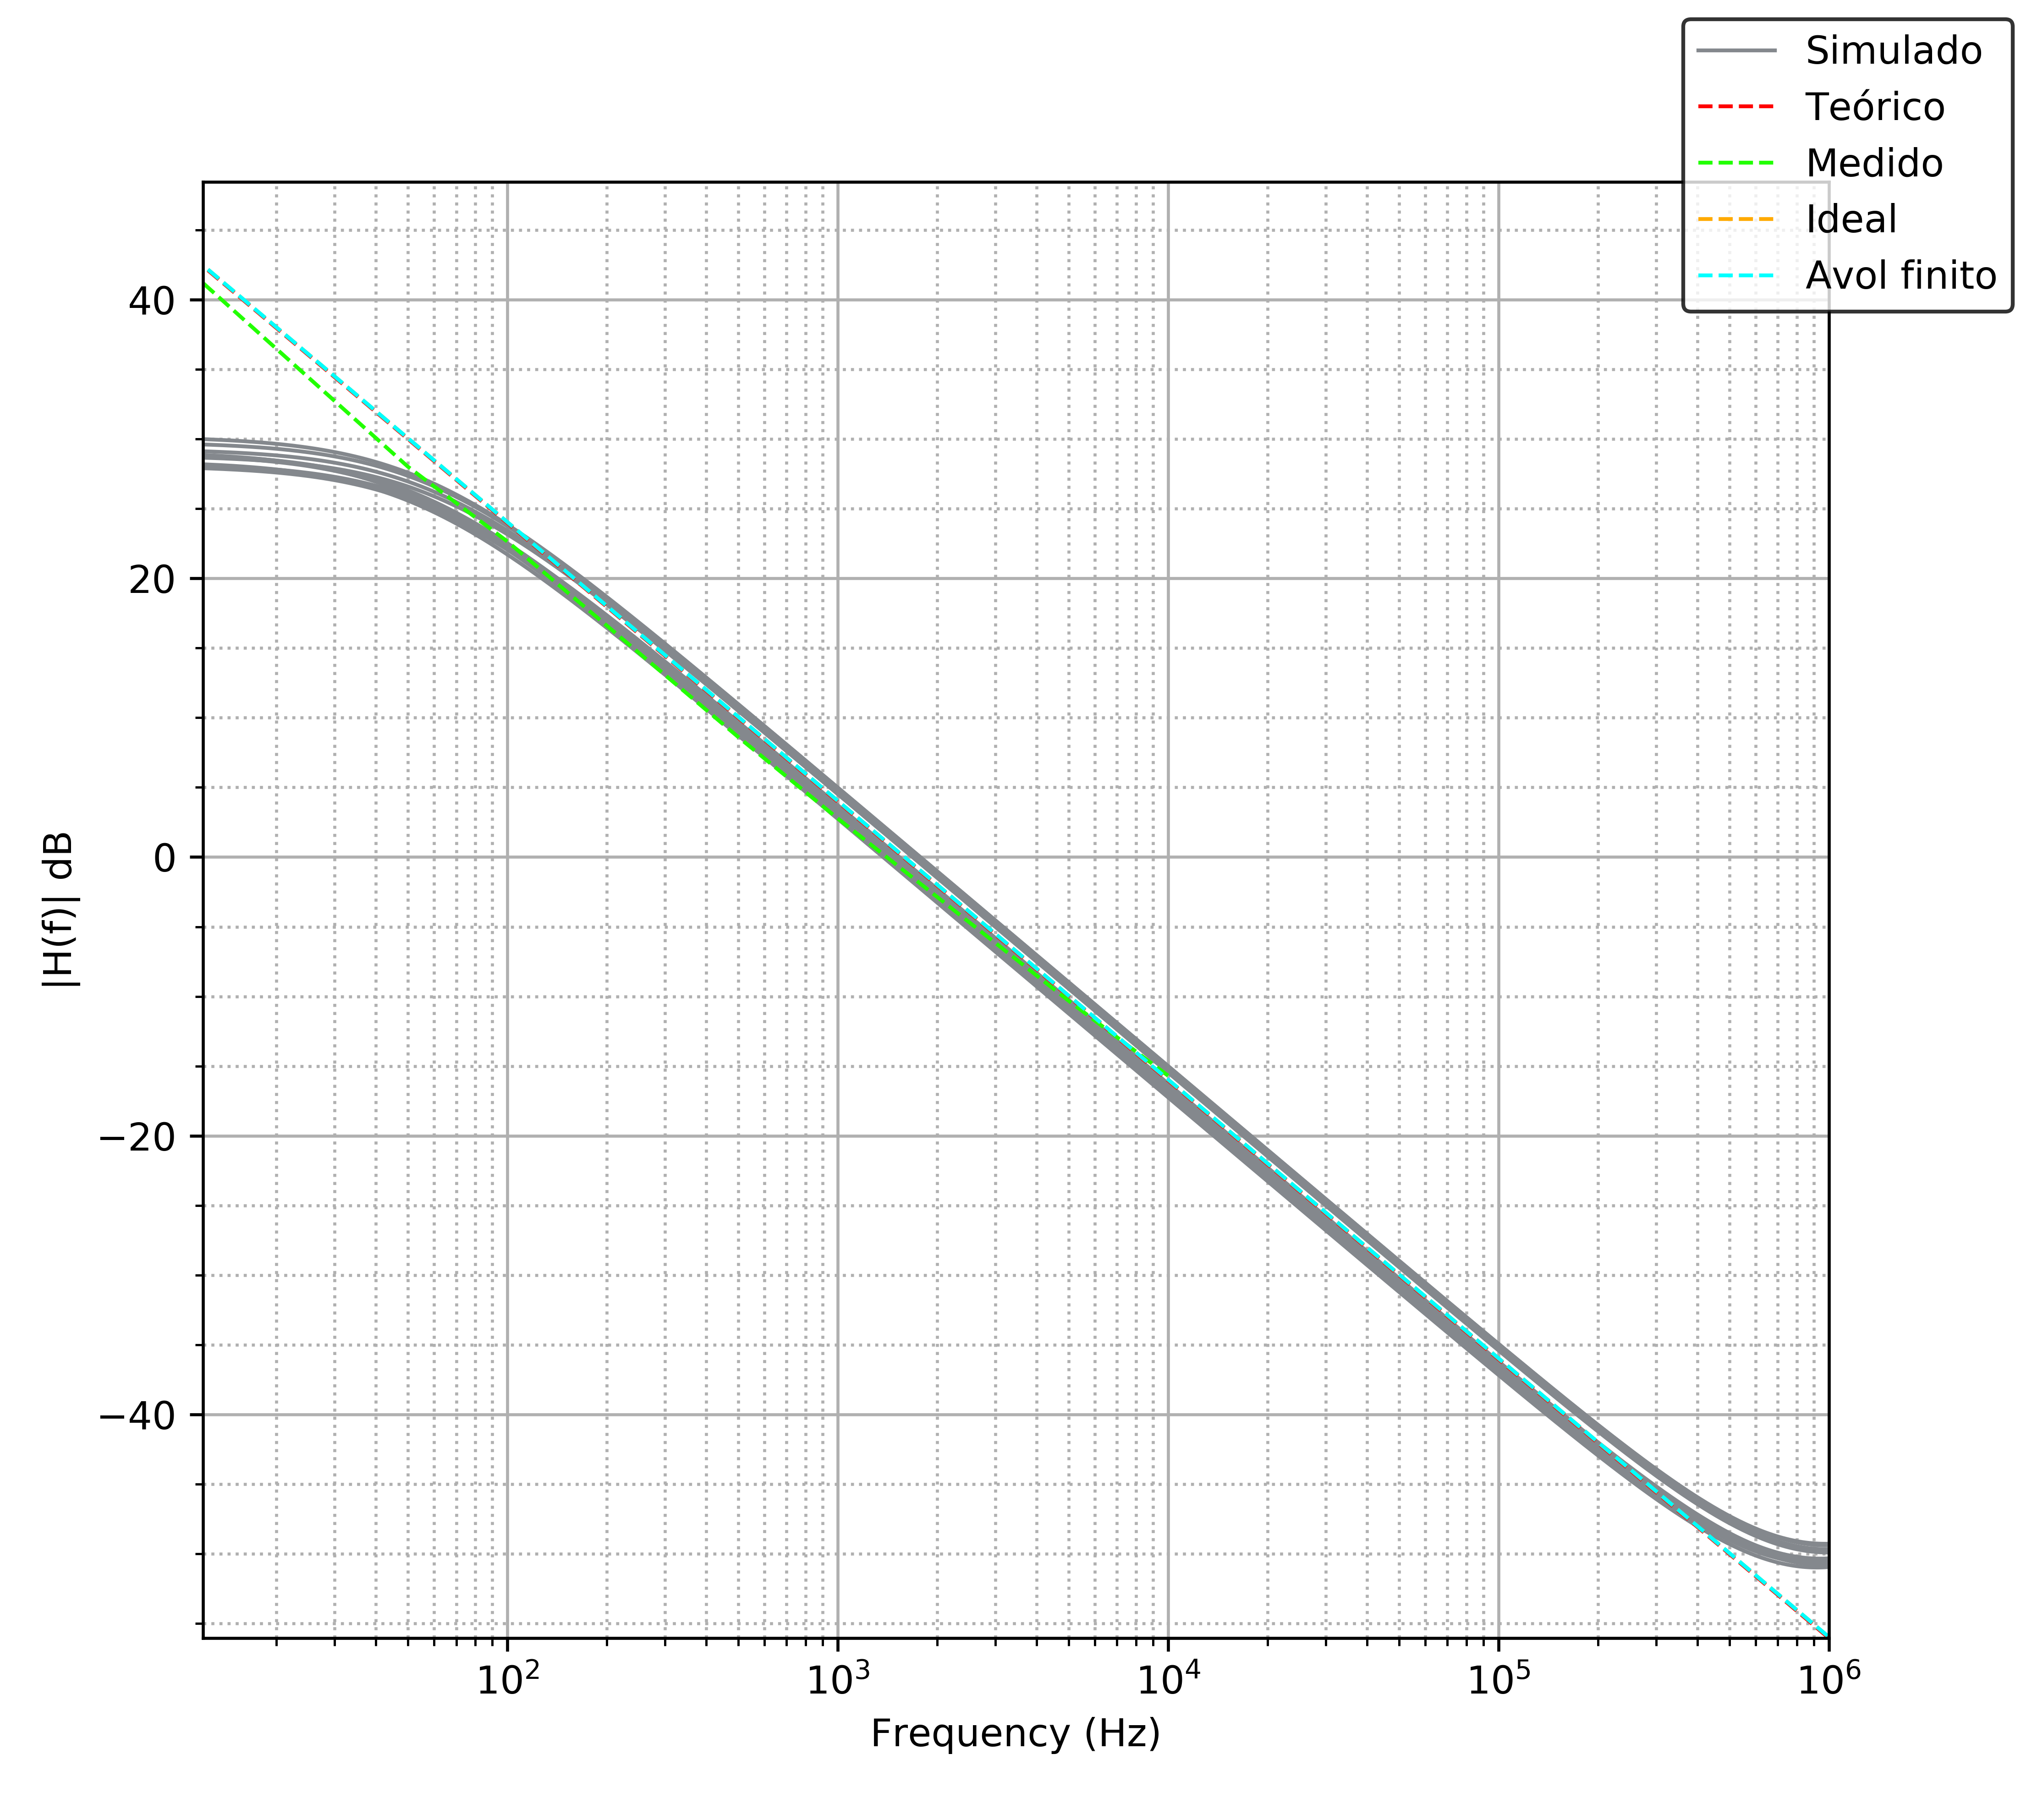
\includegraphics[scale=0.6]{Recursos/Integrador/bode_modulo.png}
	\caption{Diagrama de bode en m\'odulo del integrador sin compensar}
	\label{fig:integrador_bode_modulo}
\end{figure}

\begin{figure}[H]
	\centering
	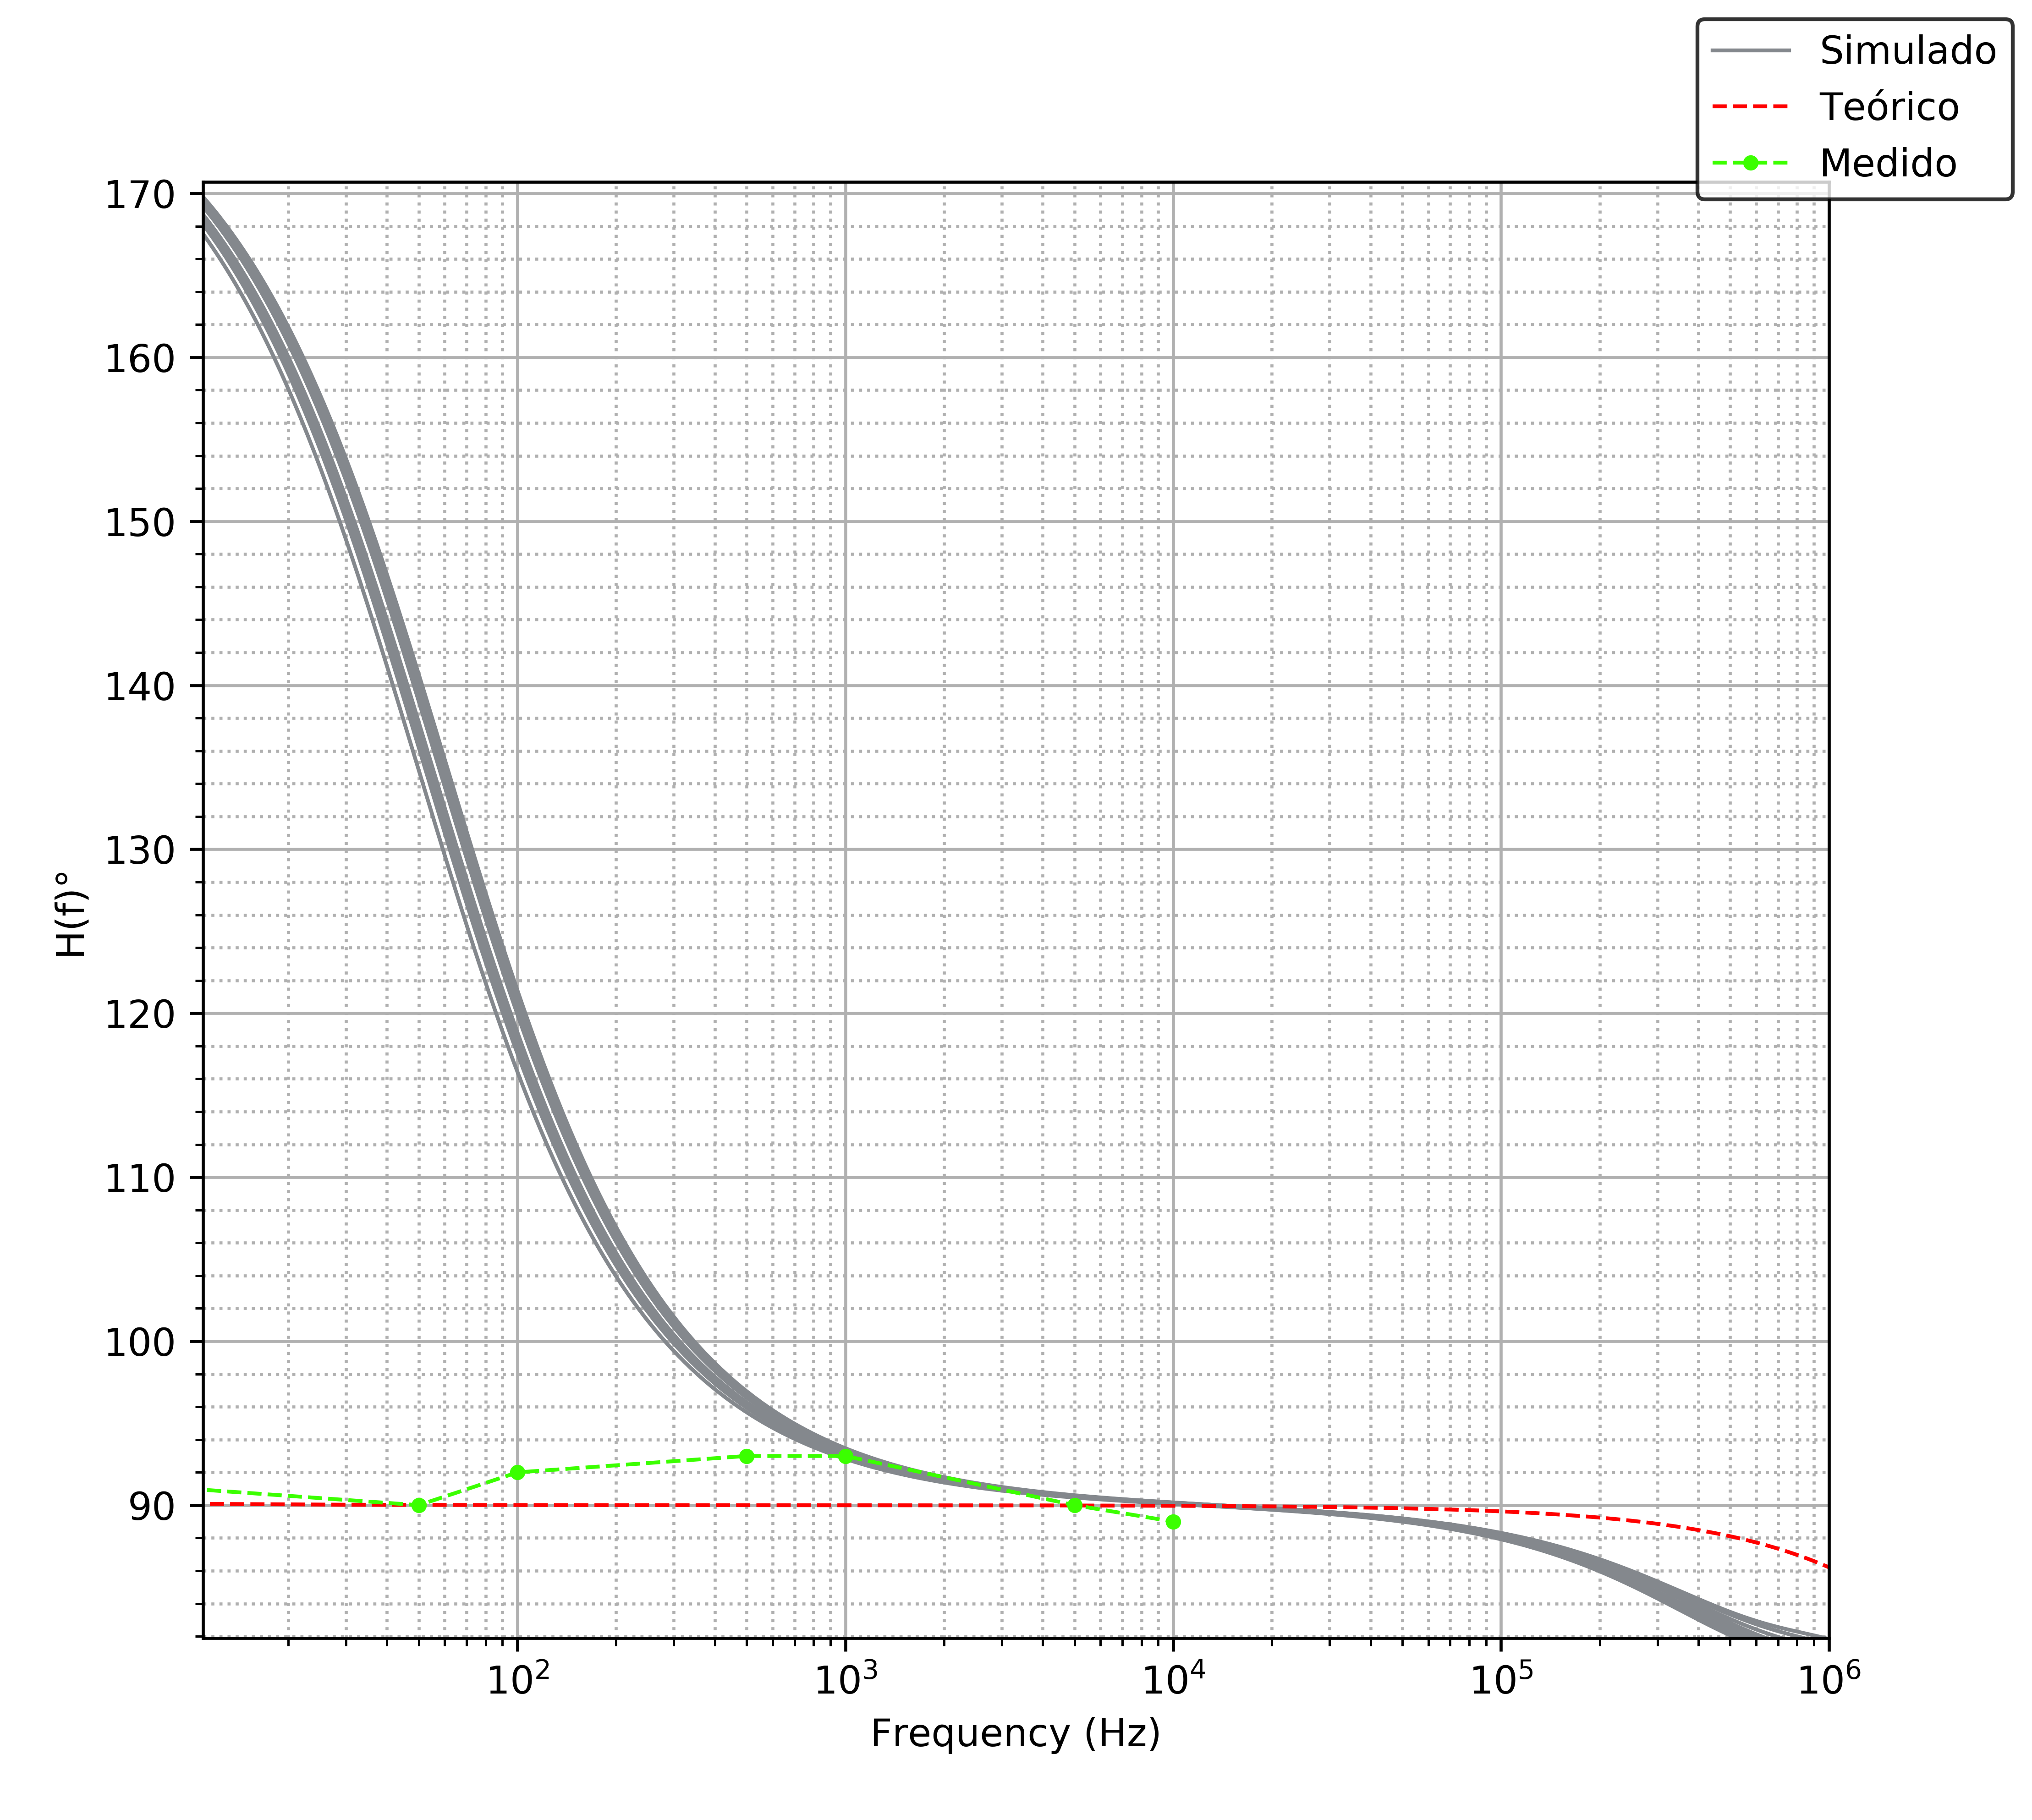
\includegraphics[scale=0.6]{Recursos/Integrador/bode_fase.png}
	\caption{Diagrama de bode en fase del integrador sin compensar}
	\label{fig:integrador_bode_fase}
\end{figure}

\paragraph*{Impedancia de entrada} en t\'erminos generales, tanto la respuesta en frecuencia como la impedancia de entrada
obtenidos en la medici\'on y en la simulaci\'on son resultados que en s\'i mismos no logran caracterizar al sistema correctamente por los efectos indeseados
de la saturaci\'on para bajas frecuencias del circuito. Esto \'ultimo tambi\'en se encuentra presente en LTSpice. En las figuras \ref{fig:integrador_simulacion} se puede observar
que seg\'un la frecuencia el nivel de continua se modifica por lo explicado anteriormente.

\begin{figure}[H]
	\centering
	\begin{tabular}{c c}
		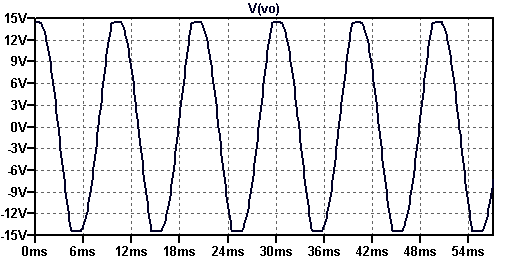
\includegraphics[scale=0.55]{Integrador/Simulaciones/Seno100.png} &
		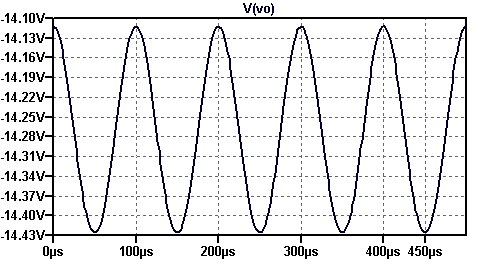
\includegraphics[scale=0.55]{Integrador/Simulaciones/Seno10k.png}
	\end{tabular}
	\caption{Respuesta del integrador sin compensar a senoidales de $100Hz$ y $10kHz$}
	\label{fig:integrador_simulacion}
\end{figure}

\begin{figure}[H]
	\centering
	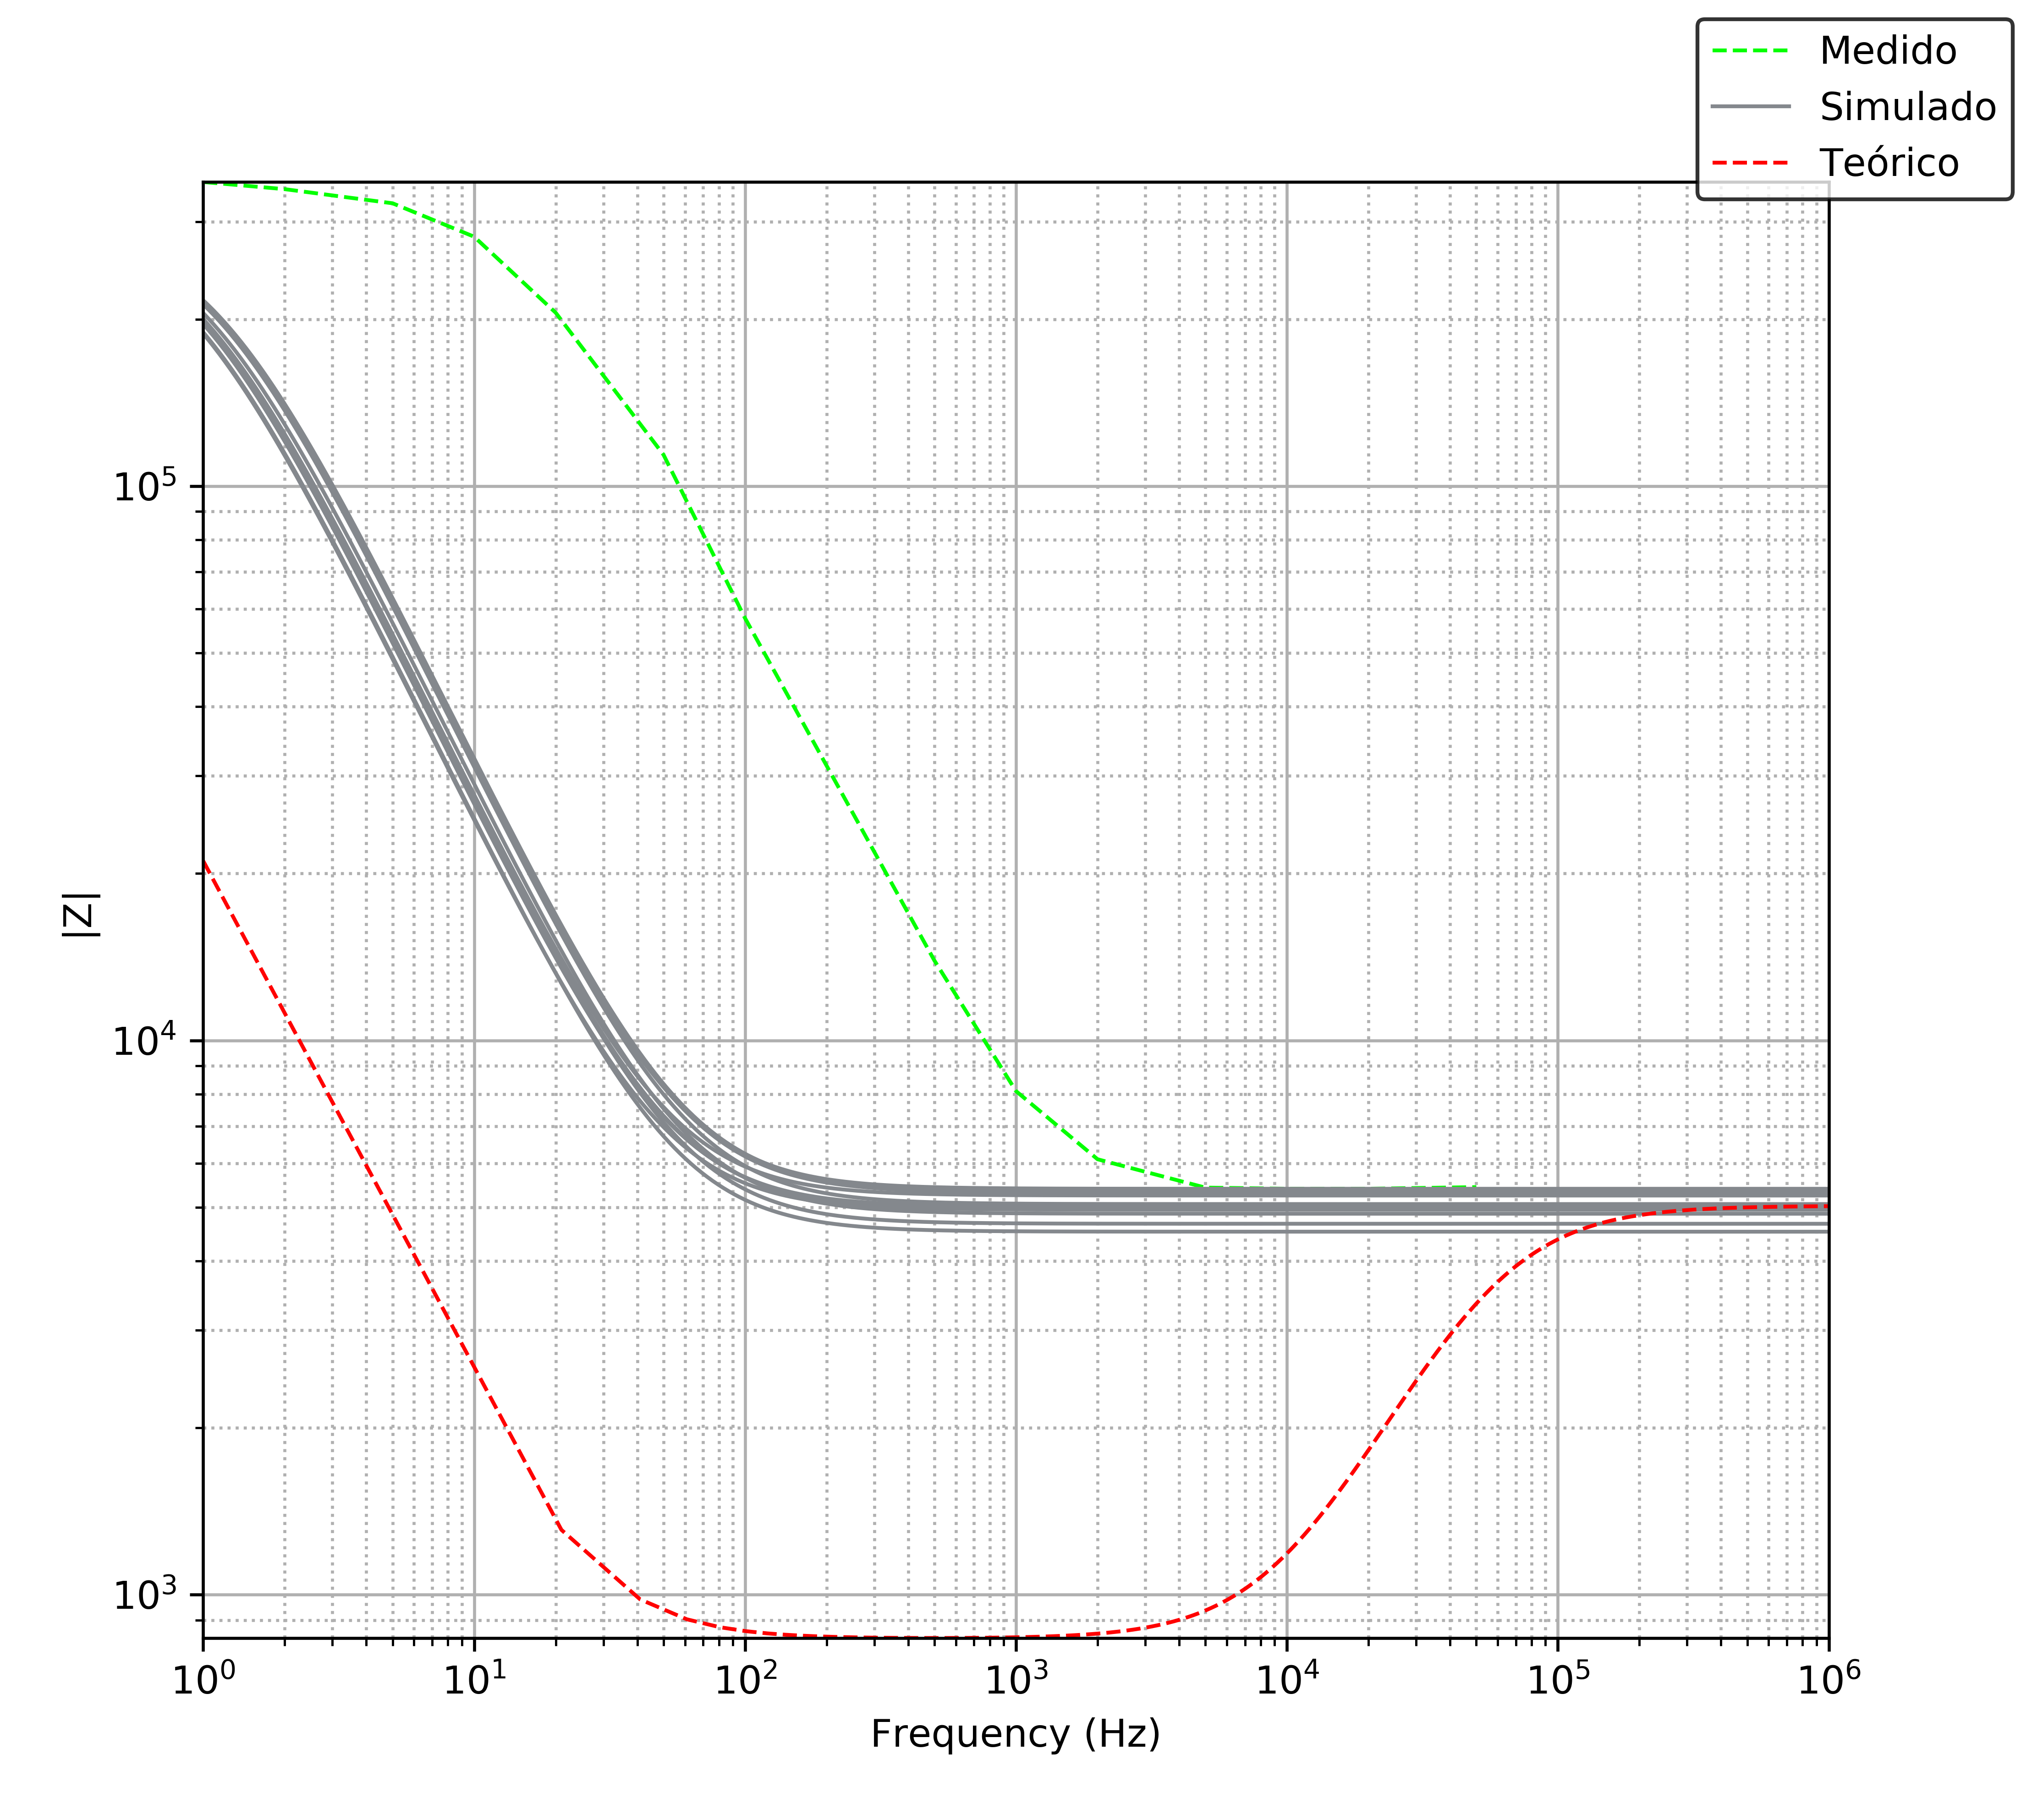
\includegraphics[scale=0.7]{Recursos/Integrador/impedancia_modulo.png}
	\caption{Impedancia de entrada en m\'odulo del integrador sin compensar}
	\label{fig:integrador_impedancia_modulo}
\end{figure}

\begin{figure}[H]
	\centering
	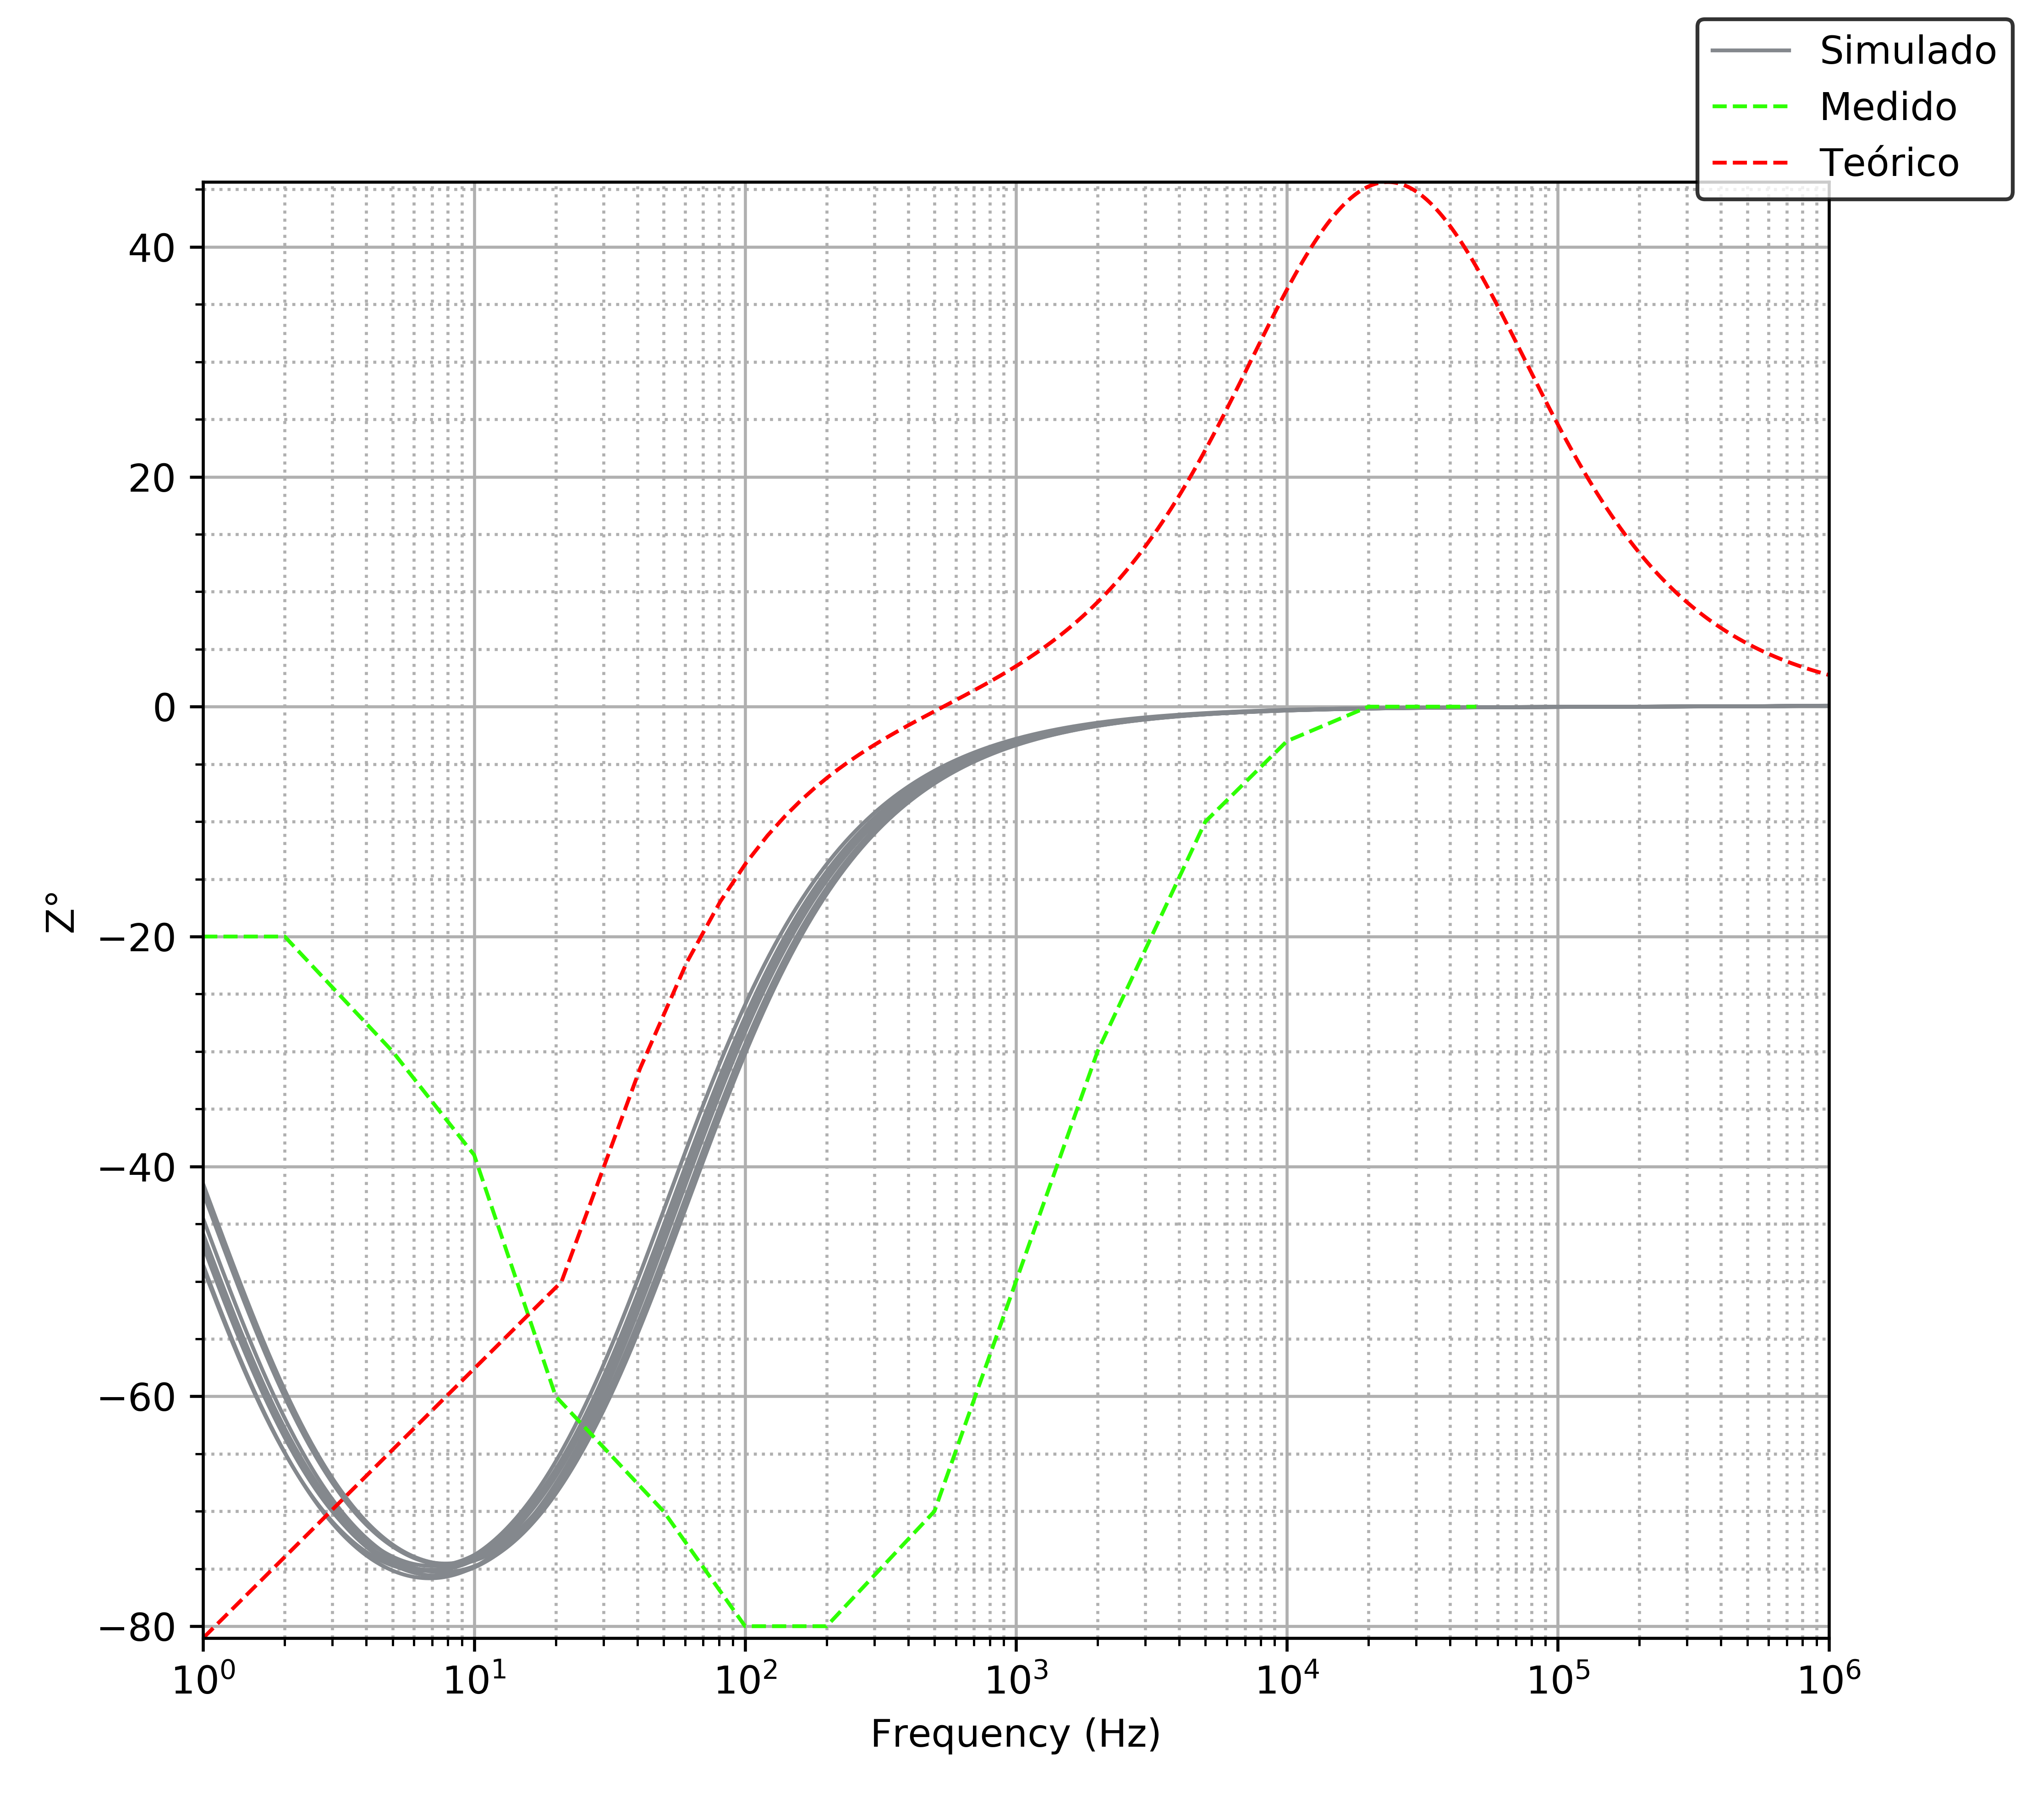
\includegraphics[scale=0.7]{Recursos/Integrador/impedancia_fase.png}
	\caption{Impedancia de entrada en fase del integrador sin compensar}
	\label{fig:integrador_impedancia_fase}
\end{figure}

\paragraph*{Respuesta a se\~nales no senoidales} A pesar de que se considera que el circuito como tal no funciona correctamente por el malfuncionamiento provocado ante las componetes de continuas,
se observ\'o la respuesta del circuito ante una se\~nal cuadrada y una se\~nal triangular, en ambos casos el resultado es en cierta forma apreciable, sin embargo se puede observar la presencia de continuas
seg\'un la frecuencia.

\begin{figure}[H]
	\centering
	\begin{tabular}{c c}
		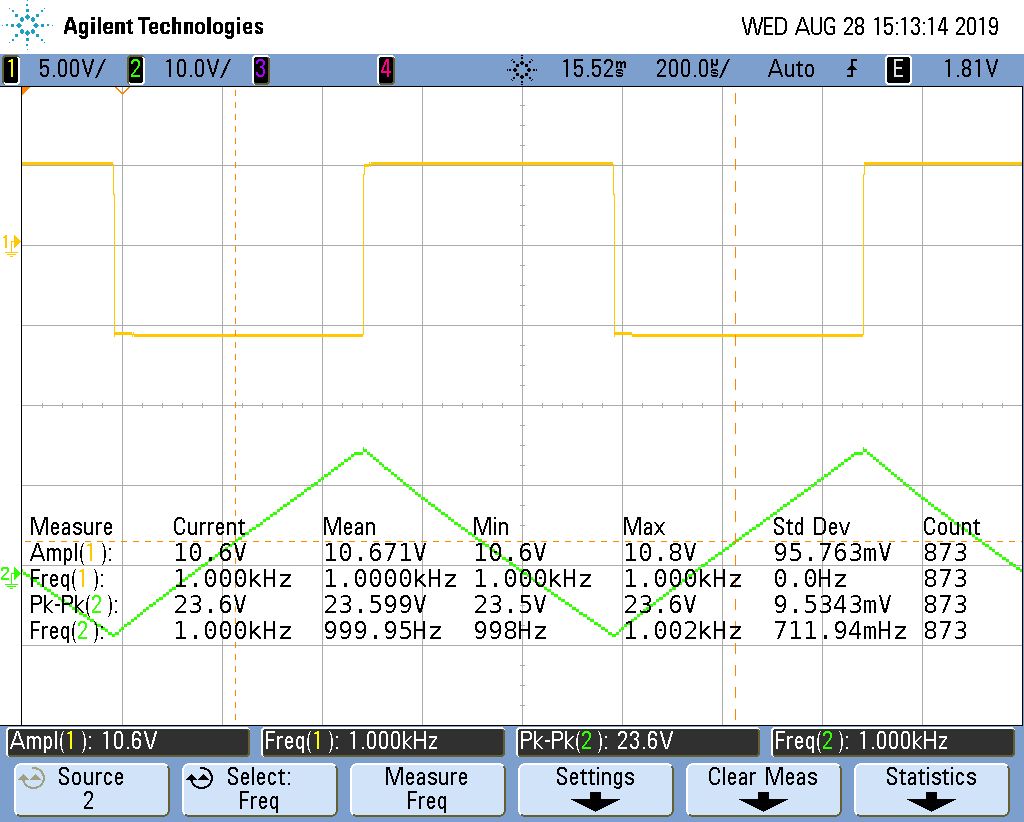
\includegraphics[scale=0.2]{Integrador/Mediciones/Osciloscopio/PCB_Sin_Compensar/osc_11.png} & 
		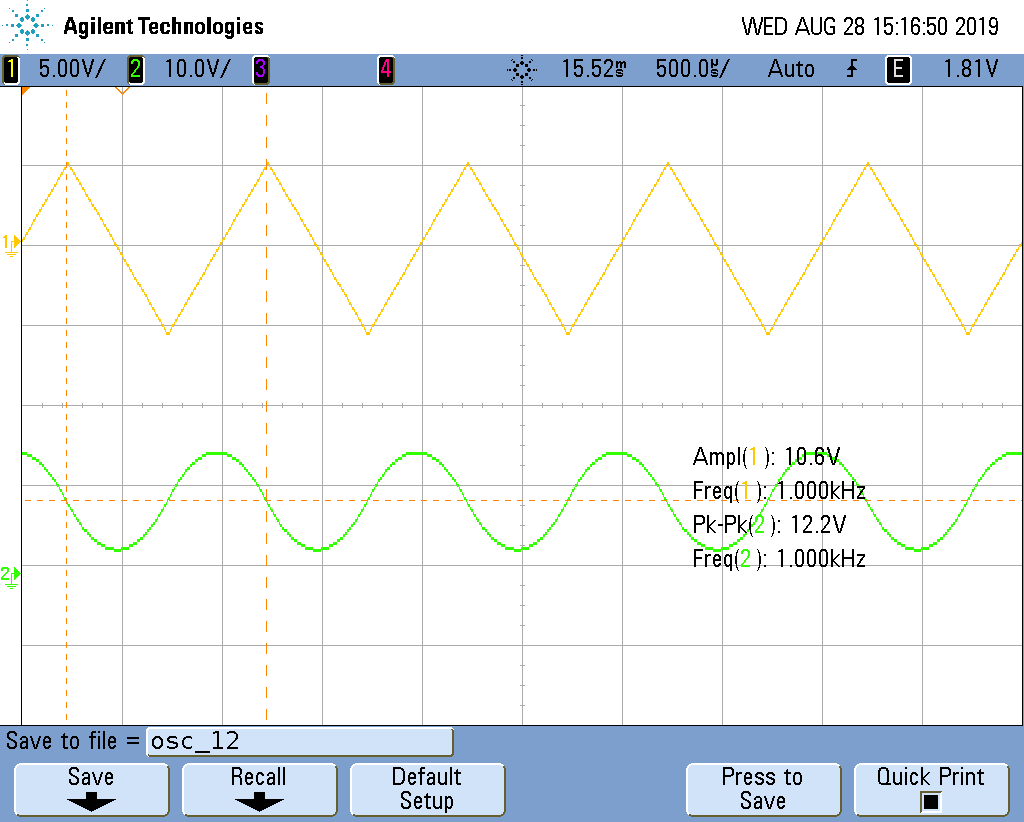
\includegraphics[scale=0.2]{Integrador/Mediciones/Osciloscopio/PCB_Sin_Compensar/osc_12.png}
	\end{tabular}
	\caption{Respuestas a se\~nales no senoidales}
	\label{fig:integrador_respuestas}
\end{figure}

	\subsection{Circuito integrador compensado}
A partir de los resultados de las mediciones y simulaciones del circuito integrador no compensado, se llega a la conclusi\'on de que como tal, el circuito no puede funcionar como integrador correctamente
y es necesario colocar una resistencia de compensaci\'on con el objetivo de limitar la ganancia para se\~nales de baja frecuencia. Por otro lado, se busca que el valor sea tal que el resultado no presente efectos no deseados como lo era para
el derivador un sobrepico por comportamientos subamortiguados, adem\'as de querer que el funcionamiento del integrador se d\'e en el mayor ancho de banda posible con un error en la fase menor a tres grados.

\subsubsection{An\'alisis Te\'orico}

\paragraph*{Funci\'on transferencia en condiciones ideales} utilizando la expresi\'on del amplificador inversor bajo condiciones ideales, se llama $Z_2$ a la impedancia que resulta del paralelo de la resistencia y el capacitor. Luego se obtiene:

\begin{equation*}
	Z_2 = R_2 // \frac{1}{s \cdot C} = \frac{R_2}{1 + s \cdot C \cdot R_2}
\end{equation*}

\begin{equation}
	H(s) = \frac{V_o(s)}{V_i(s)} = - \frac{Z_2}{R_1} = - \frac{\frac{R_2}{R_1}}{1 + s \cdot C \cdot R_2}
	\label{eq:integrador_compensado_transfer_ideal}
\end{equation}

\paragraph*{Funci\'on transferencia con $A_{vol}$ finito} considerando la misma impedancia del paralelo en la realimentaci\'on que en la resoluci\'on ideal, se calcula el valor del potencial en la pata inversora del amplificador operacional y luego se halla la expresi\'on de la funci\'on de la siguiente manera:

\begin{equation*}
	v^{-} = V_o \cdot \frac{R_1}{R_1+ Z_2} + V_i \cdot \frac{Z_2}{Z_2 + R_1} \Rightarrow
	v^{-} = \frac{V_o \cdot R_1 \cdot ( 1 + s \cdot C \cdot R_2) + V_i \cdot R_2}{R_2 + R_1 \cdot (1 + s \cdot C \cdot R_2)}
\end{equation*}

\begin{align*}
	V_o = (v^{+} - v^{-}) \cdot A_{vol} = - A_{vol} \cdot \frac{V_o \cdot R_1 \cdot ( 1 + s \cdot C \cdot R_2) + R_2 \cdot V_i}{R_1 + R_2 + s \cdot C \cdot R_1 \cdot R_2} \Rightarrow \\
	V_o \cdot \left[ 1 + \frac{A_{vol} \cdot R_1 \cdot ( 1 + s \cdot C \cdot R_2)}{R_1 + R_2 + s \cdot C \cdot R_1 \cdot R_2} \right] =
	V_i \cdot \frac{-A_{vol} \cdot R_2}{R_1 + R_2 + s \cdot C \cdot R_1 \cdot R_2} 
\end{align*}

\begin{equation}
	H(s) = \frac{- A_{vol} \cdot R_2}{R_1 \cdot ( 1 + A_{vol} ) + R_2} \cdot \frac{1}{1 + s \cdot \frac{C \cdot R_1 \cdot R_2 \cdot ( 1 + A_{vol})}{R_1 \cdot (1 + A_{vol}) + R_2}}
	\label{eq:integrador_compensado_transfer_avol_finito}
\end{equation}

\paragraph*{Funci\'on transferencia con polo dominante} luego reemplazando en la expresi\'on anterior la forma del $A_{vol}(\omega)$ se obtiene:

\begin{equation*}
	H(s) = \frac{-A_o \cdot \omega_p \cdot R_2}{R_1 \cdot ( A_o \cdot \omega_p + s + \omega_p) + R_2 \cdot (s + \omega_p)} \cdot \frac{1}{1 + s \cdot \frac{C \cdot R_1 \cdot R_2 \cdot ( A_o \cdot \omega_p + s + \omega_p)}{R_2 \cdot ( s + \omega_p) + R_1 \cdot (A_o \cdot \omega_p + s + \omega_p)}}
\end{equation*}

\begin{equation}
	H(s) = \frac{-A_o \cdot R_2}{R_2 + R_1 \cdot (1+A_o)} \cdot \frac{1}{1 + s \cdot \frac{C \cdot R_1 \cdot R_2 \cdot \omega_p \cdot (A_o + 1) + R_1 + R_2}{\omega_p \cdot (R_2 + R_1 \cdot(A_o + 1))} + s^{2} \cdot \frac{C \cdot R_1 \cdot R_2}{\omega_p \cdot (R_2 + R_1 \cdot (A_o + 1))}}
	\label{eq:integrador_compensado_transfer_polo_dominante}
\end{equation}

\paragraph*{Impedancia de entrada con $A_{vol}$ finito} llamando como $Z_2$ al paralelo entre la resistencia y el capacitor en el lazo de la realimentaci\'on y luego aplicando ley de nodos, se obtiene:

\begin{align*}
	I_1 & = I_2 + I_3 \Rightarrow \frac{V_i + V_d}{R_1} = \frac{-V_d}{R_{id}} + \frac{-V_d - V_d \cdot A_{vol}}{Z_o + Z_2}\\
	& \Rightarrow
	V_d = \frac{- V_i \cdot r_{id} \cdot \left[ R_2 + Z_o \cdot (1 + s \cdot C \cdot R_2) \right]}{(R_1 + r_{id}) \cdot \left[R_2 + Z_o \cdot (1 + s \cdot C \cdot R_2) \right] + (1 + A_{vol}) \cdot ( 1 + s \cdot C \cdot R_2) \cdot R_1 \cdot r_{id}}
\end{align*}

\begin{align}
	Z_{in}(s) = \frac{V_i}{I_1} = \frac{(R_1 + r_{id}) \cdot (R_2 + Z_o) + (1 + A_{vol}) \cdot (R_1 + r_{id})}{R_2 + Z_o + r_{id} \cdot(1 + A_{vol})} \cdot \frac{1 + s \cdot \frac{C \cdot R_2 \cdot \left[ Z_o \cdot (R_1 + r_{id}) + R_1 \cdot r_{id} \cdot ( 1 + A_{vol}) \right]}{(R_1 + r_{id}) \cdot (R_2 + Z_o) + (1 + A_{vol}) \cdot R_1 \cdot r_{id}}}{1 + s \cdot \frac{C \cdot R_2 \left[ Z_o + r_{id} \cdot ( 1 + A_{vol}) \right]}{R_2 + Z_o + r_{id} \cdot ( 1 + A_{vol})}}
\end{align}

\paragraph*{Impedancia de entrada con polo dominante} reemplazando $A_{vol}$ por su expresi\'on incluyendo el polo dominante, se llega luego de unos pasos algebraicos a que:

\begin{align}
	Z_{in}(s) = \frac{(R_1+r_{id})\cdot(R_2 + Z_o) + R_1 \cdot r_{id} \cdot(1+A_o)}{R_2 + Z_o + r_{id} \cdot(1 + A_o)} \cdot \frac{1 + s \cdot \beta + s^{2} \cdot \alpha}{1 + s \cdot b + s^{2} \cdot a }
\end{align}

\begin{align*}
	a & = \frac{C \cdot R_2 \cdot (Z_o + r_{id})}{\omega_p \cdot \left[ R_2 + Z_o + r_{id} \cdot(1 + A_o) \right]} \\
	b & = \frac{R_2 + Z_o + r_{id} + \omega_p \cdot C \cdot R_2 \cdot \left[ Z_o + (1 + A_o) \cdot r_{id} \right] }{\omega_p \cdot \left[ R_2 + Z_o + r_{id} \cdot(1 + A_o) \right] } \\
	\alpha & = \frac{C \cdot R_2 \cdot \left[ (R_1 + r_{id}) \cdot Z_o + R_1 \cdot r_{id} \right] }{\omega_p \left[ (R_1 + r_{id}) \cdot (R_2 + Z_o) + R_1 \cdot r_{id} \cdot(1 + A_o) \right]} \\
	\beta & = \frac{(R_1 + r_{id}) \cdot \left[C \cdot R_2 \cdot Z_o \cdot \omega_p + R_2 + Z_o \right] + R_1 \cdot r_{id} \cdot \left[ 1 + C \cdot R_2 \cdot \omega_p \cdot (A_o + 1) \right] }{\omega_p \left[ (R_1 + r_{id}) \cdot (R_2 + Z_o) + R_1 \cdot r_{id} \cdot(1 + A_o) \right] }
\end{align*}

\paragraph*{Expresiones finales} para finalizar con el dise\~no y an\'alisis te\'orico del integrador compensado es necesario determinar el valor de la resistencia de compensaci\'on que debe ser colocada en paralelo
al capacitor, para que de esta forma se logre que en bajas frecuencias cuando el lazo de realimentaci\'on por el capacitor se ve debilitado, la resistencia mantenga tal realimentaci\'on. Por otro lado, a dicha resistencia se le imponen
las condiciones mencionadas al principio de esta secci\'on, estas son, que no presente sobrepicos la respuesta en frecuencia, que integre en el mayor rango de frecuencias con un error de fase menor a 3 grados y se logre compensar
efectivamente el circuito.

Para lograr estas condiciones, se propone an\'alizar te\'oricamente cu\'ales son las componentes de corriente continua del $LM833$ que pueden provocar la saturaci\'on
del integrador incluso cuando no hay entrada. Para ello se analiza el efecto de las corrientes de bias y la tensi\'on de polarizaci\'on del amplificador operacional.
Analizando la hoja de datos, se obtiene que la corriente de bias tiene un valor de $I_{io} = 200nA$ y la tensi\'on de polarizaci\'on es de
$V_{io} = 5mV$. Utilizando esto para limitar el valor de tensi\'on de salida de forma que no haya saturaci\'on y considerando que el circuito se encuentra configurado
de forma \'optima para el menor efecto de las corrientes de bias, se encuentra que la componente de salida de continua y sobre ella se imponen tales restricciones, considerando que en el peor caso se quiere una tensi\'on de salida m\'axima de $V_{max} = 1V$ simplemente 
para tener un valor de resistencia de referencia que no se puede sobrepasar
, y luego imponiendo como una condici\'on adicional, que la frecuencia de corte como m\'axmio debe estar ubicada en aproximadamente $f_o = 20Hz$ para
 lograr un ancho de banda amplio dentro del cual se integre correctamente, se llega a que:

\begin{equation*}
	V_{dc} = (200nA) \cdot R_2 + 5mV \cdot ( 1 + \frac{R_2}{R_1} )
	\Rightarrow
	R_2 < 829,16 k \Omega 
\end{equation*}

\begin{align*}
	f_o & = \frac{1}{2 \pi \cdot C \cdot R_2} 
	\Rightarrow
	R_2 > \frac{1}{2 \pi \cdot C \cdot f_o}
	\Rightarrow
	R_2 > 397,89k \Omega
\end{align*}

En consecuencia se opta por tomar un valor de resistencia $R_2 = 470k\Omega$ puesto que ajusta correctamente en el rango de los criterios adoptados.

\begin{equation}
	H(s) = \frac{-93,91}{1 + s \cdot 9,392 \cdot 10^{-3} + \left( \frac{s}{2 \pi \cdot 15,94kHz} \right)^{2}}
\end{equation}

>>>>>>> 1c903573e405a1b067e44751a5fd15495a8566b3
\begin{equation}
	Z_{in}(s) = \frac{5000 + s \cdot 46,995 + s^{2} \cdot 5,02 \cdot 10^{-7}}{1 + s \cdot 9,39 \cdot 10^{-3} + s^{2} \cdot 9,975 \cdot 10^{-11}}
\end{equation}

	\subsubsection{Resultados}
Antes de presentar los resultados obtenidos a este circuito, es importante aclarar que al momento de realizar las mediciones, cuando se utilizaban entradas
al circuito integrador compensado con altas frecuencias suced\'ia que la salida se ve\'ia atenuada demasiado, con lo cual a pesar de haber tomado algunas mediciones 
para esos extremos, se decidi\'o no incluirlas ni tomar valores en ese rango tan amplio porque se obten\'ian resultados que no eran apreciables.

\paragraph*{Respuesta en frecuencia} se puede observar en lo gr\'aficos obtenidos, que el circuito integrador compensado
contrasta te\'oricamente con las mediciones y simulaciones, a pesar de algunas diferencias en la fase para bajas frecuencias. No obstante,
como se puede observar, la fase se mantiene en aproximadamente $90^{\circ}$ para un rango de frecuencias de $ 1kHz < f < 500kHz $, si consideramos como
la regi\'on v\'alida para integraci\'on aquella donde la desviaci\'on no supera los 3 grados como fue consignado.

\begin{table}[H]
	\centering
	\begin{tabular}{c c c c c}%
		$V_{gen} [V]$ & $f_{gen} [Hz]$ & $V_{out} [V]$ & $\phase{V_{out}} [\circ]$ & $\frac{V_o}{V_i} [dB]$ \\ \hline
		\csvreader[head to column names, late after line=\\]{bode.csv}{}{\in & \f & \out & \p & \db}
		\hline
	\end{tabular}
\end{table}

\begin{figure}[H]
	\centering
	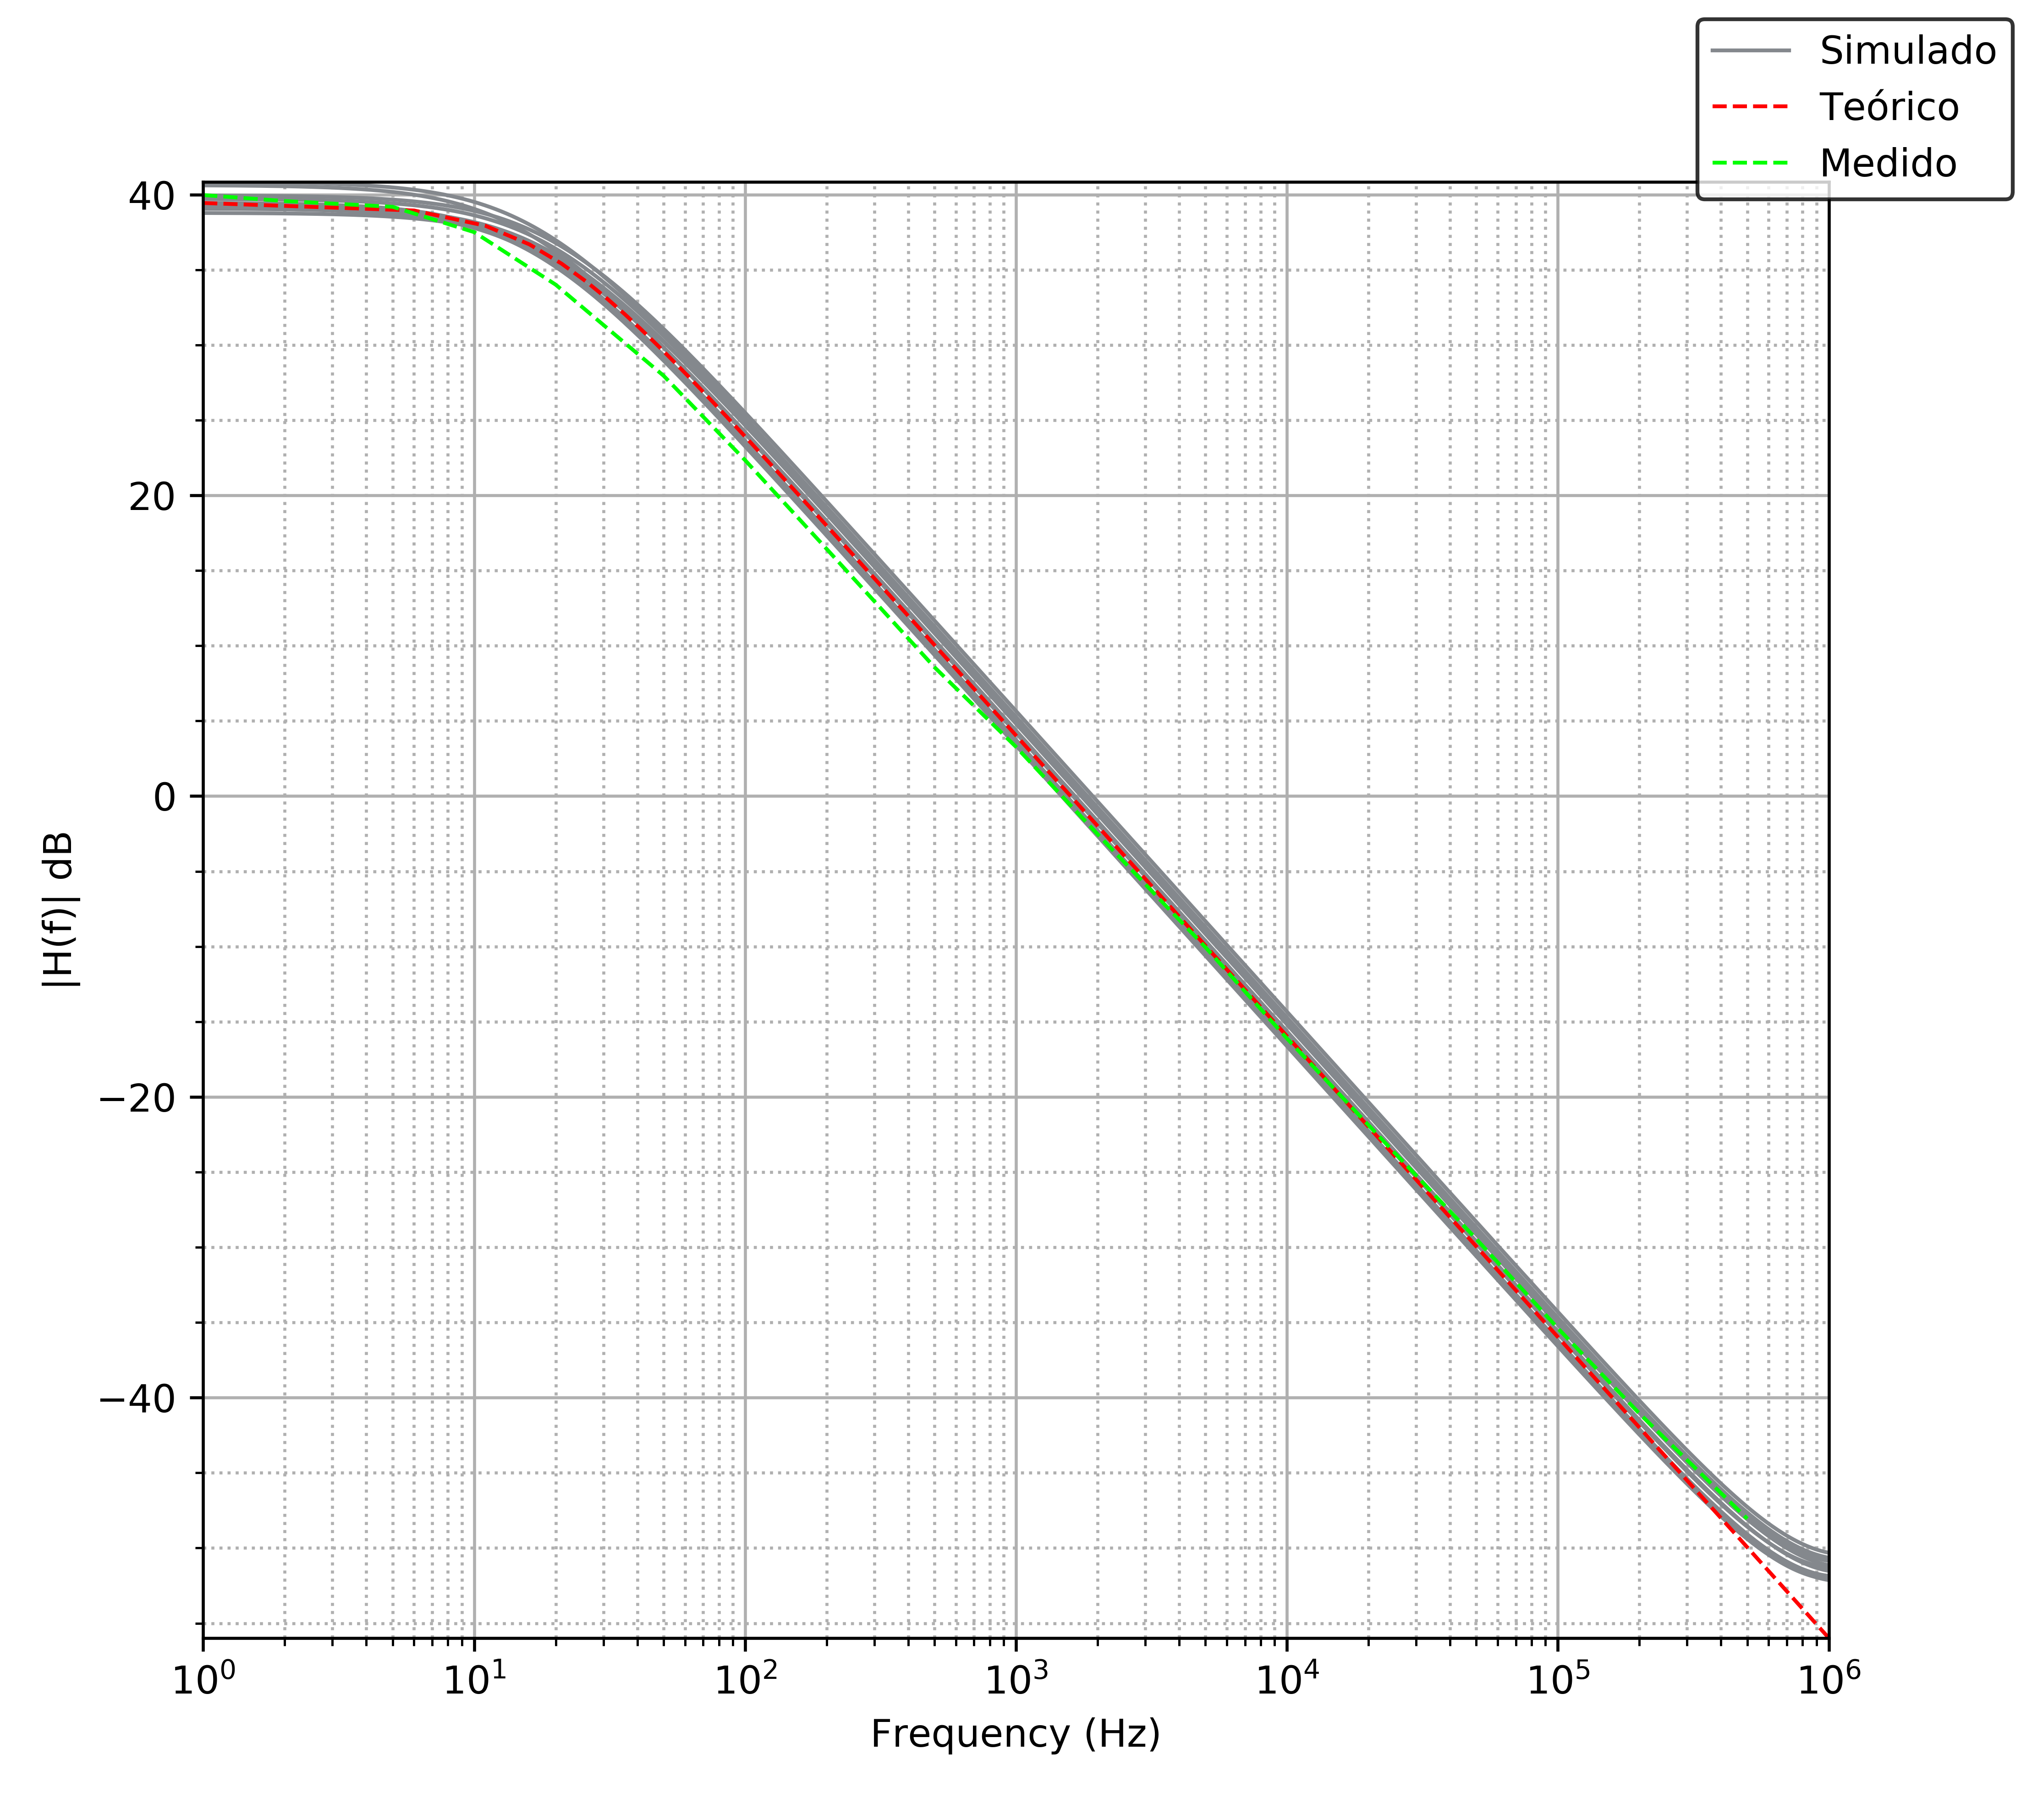
\includegraphics[scale=0.6]{Recursos/Integrador_compensado/bode_modulo.png}
	\caption{Diagrama de bode en m\'odulo del circuito integrador compensado}
	\label{fig:integrador_compensado_bode_modulo}
\end{figure}

\begin{figure}[H]
	\centering
	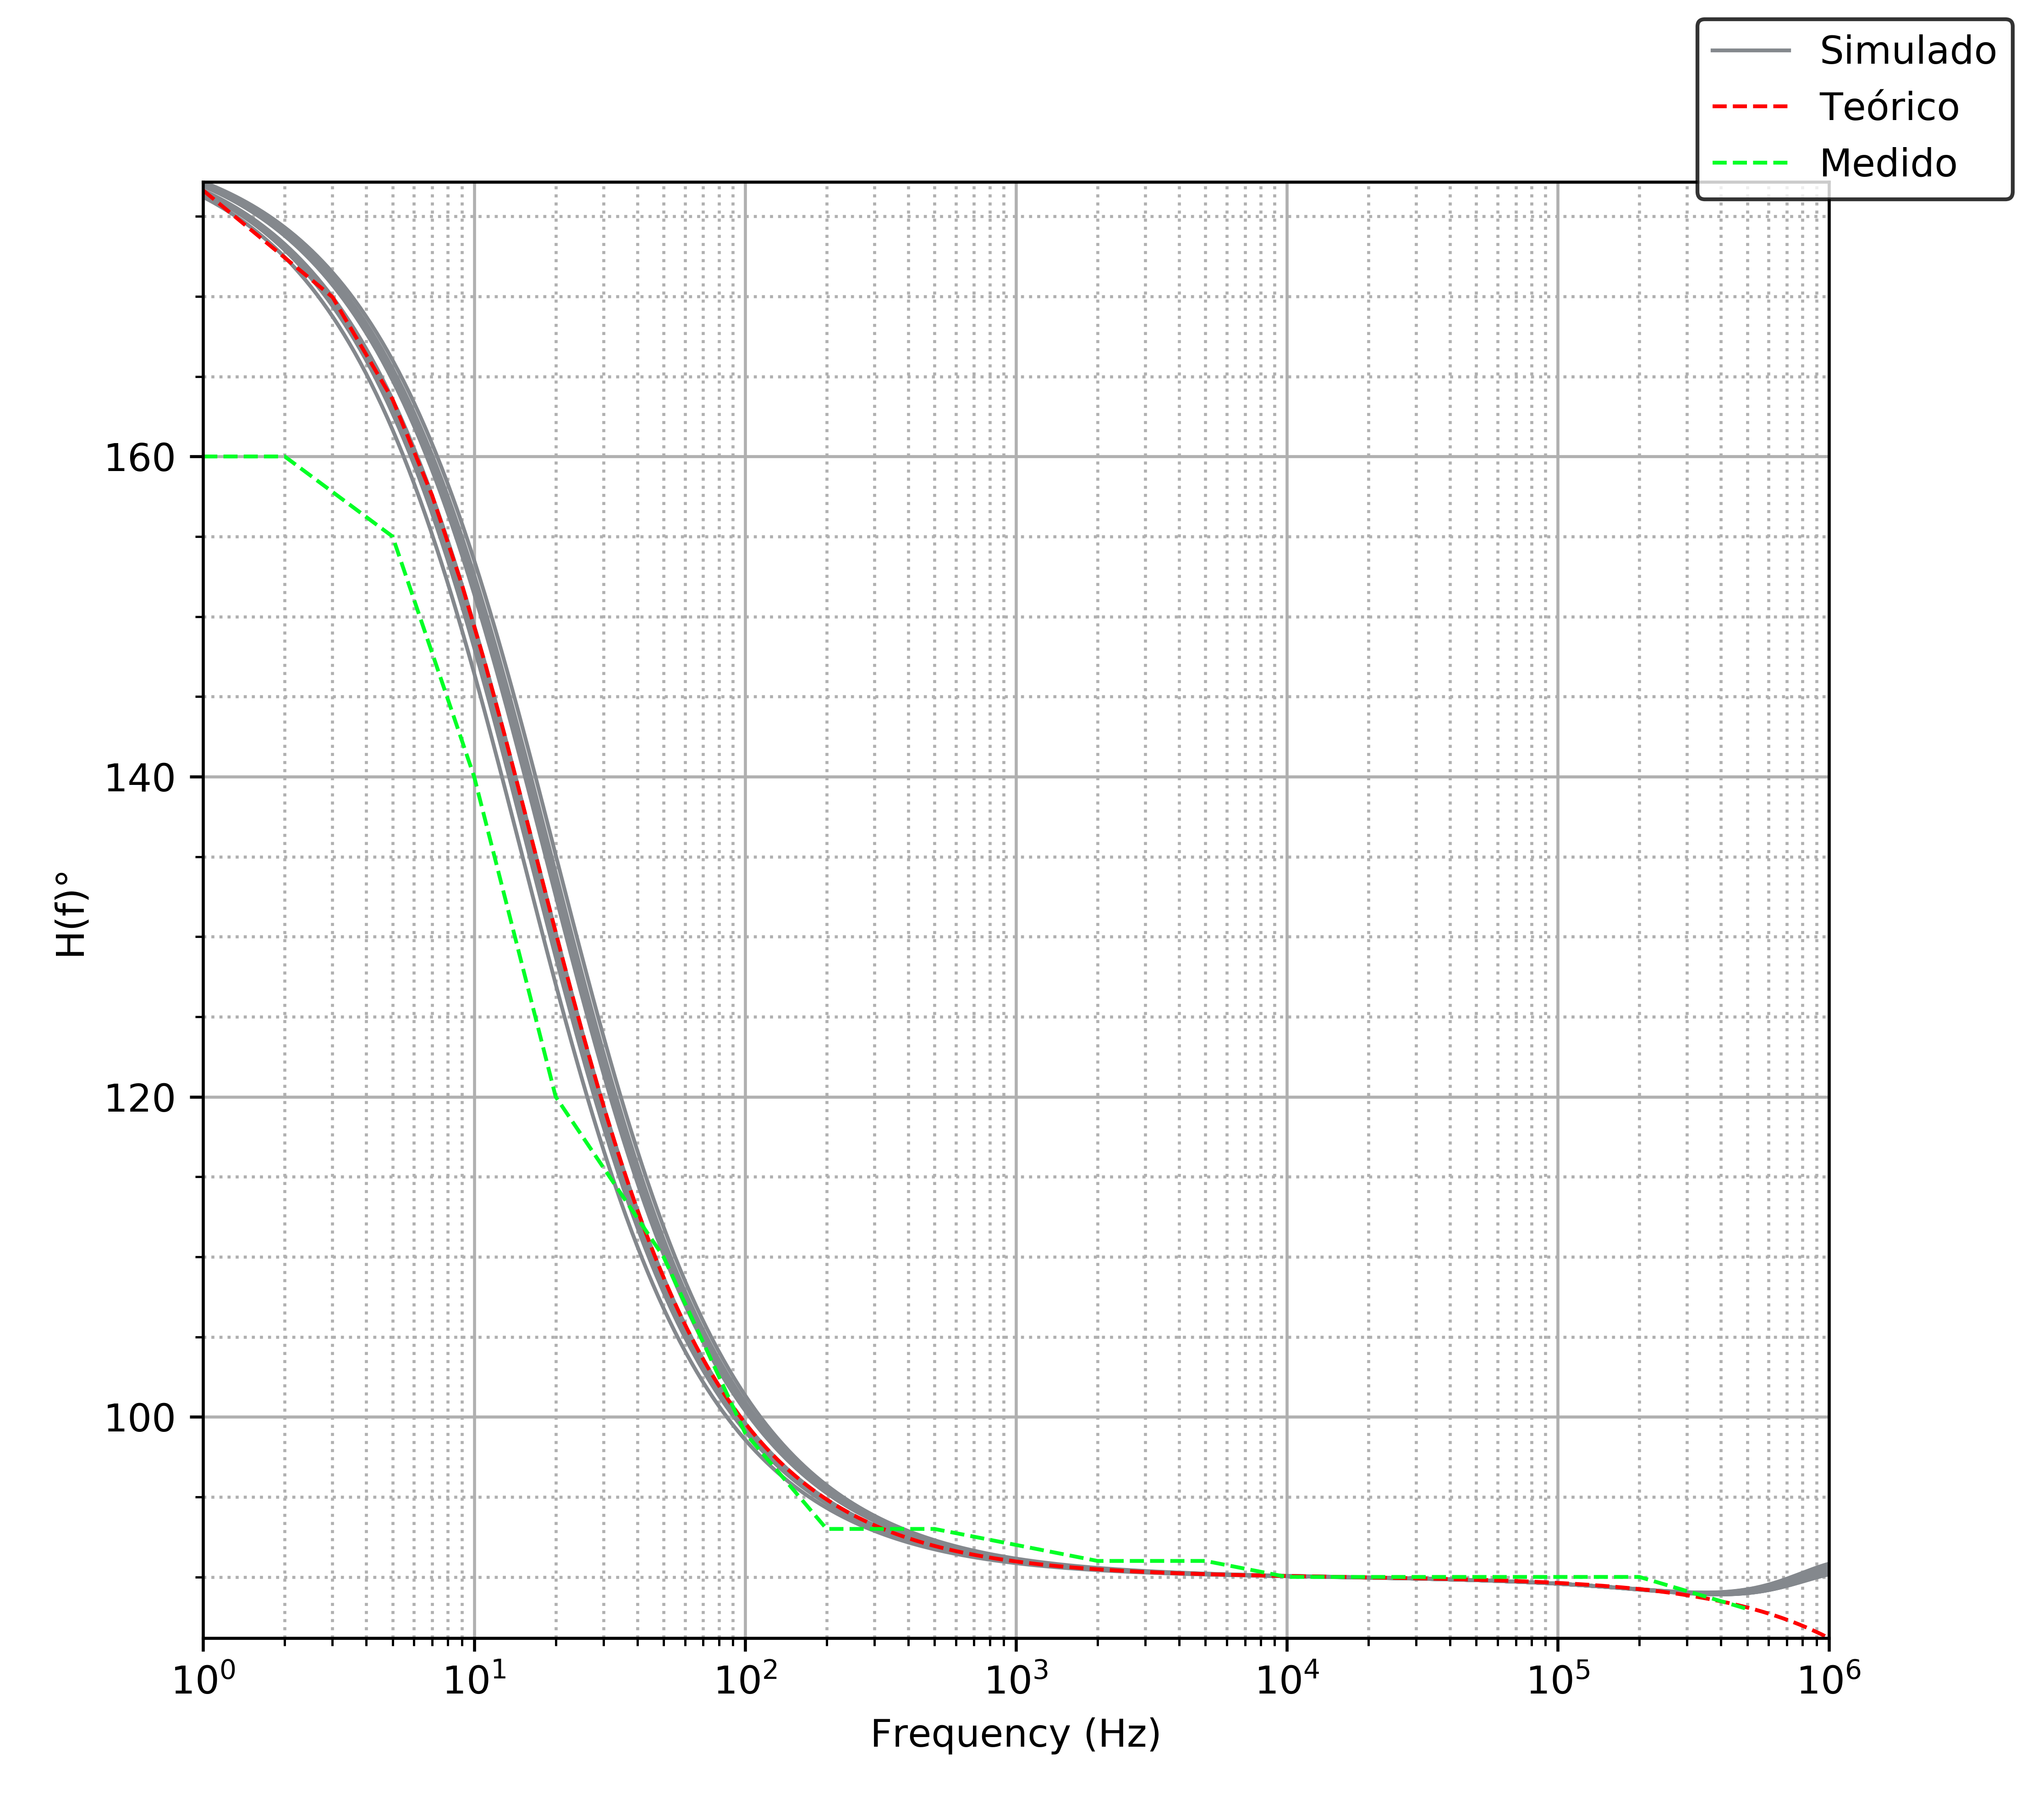
\includegraphics[scale=0.6]{Recursos/Integrador_compensado/bode_fase.png}
	\caption{Diagrama de bode en fase del circuito integrador compensado}
	\label{fig:integrador_compensado_bode_fase}
\end{figure}

\paragraph*{Impedancia de entrada} se puede observar en las curvas obtenidas de la simulaci\'on, la medici\'on y los c\'alculos
te\'oricos, que la fase contrasta con muy poco error, no obstante en las mediciones del m\'odulo tiene un valor medio de 
$|Z_{in}| = 5,25k \Omega$ con un error medio de $E_r = 5,02\% $. Dado que el error se da para toda frecuencia, no se puede asumir que las puntas
de osciloscopio hayan tenido una implicancia, se atribuye el error de la impedancia a las desviaciones provocadas por la tolerancia de los componentes.

\begin{figure}[H]
	\centering
	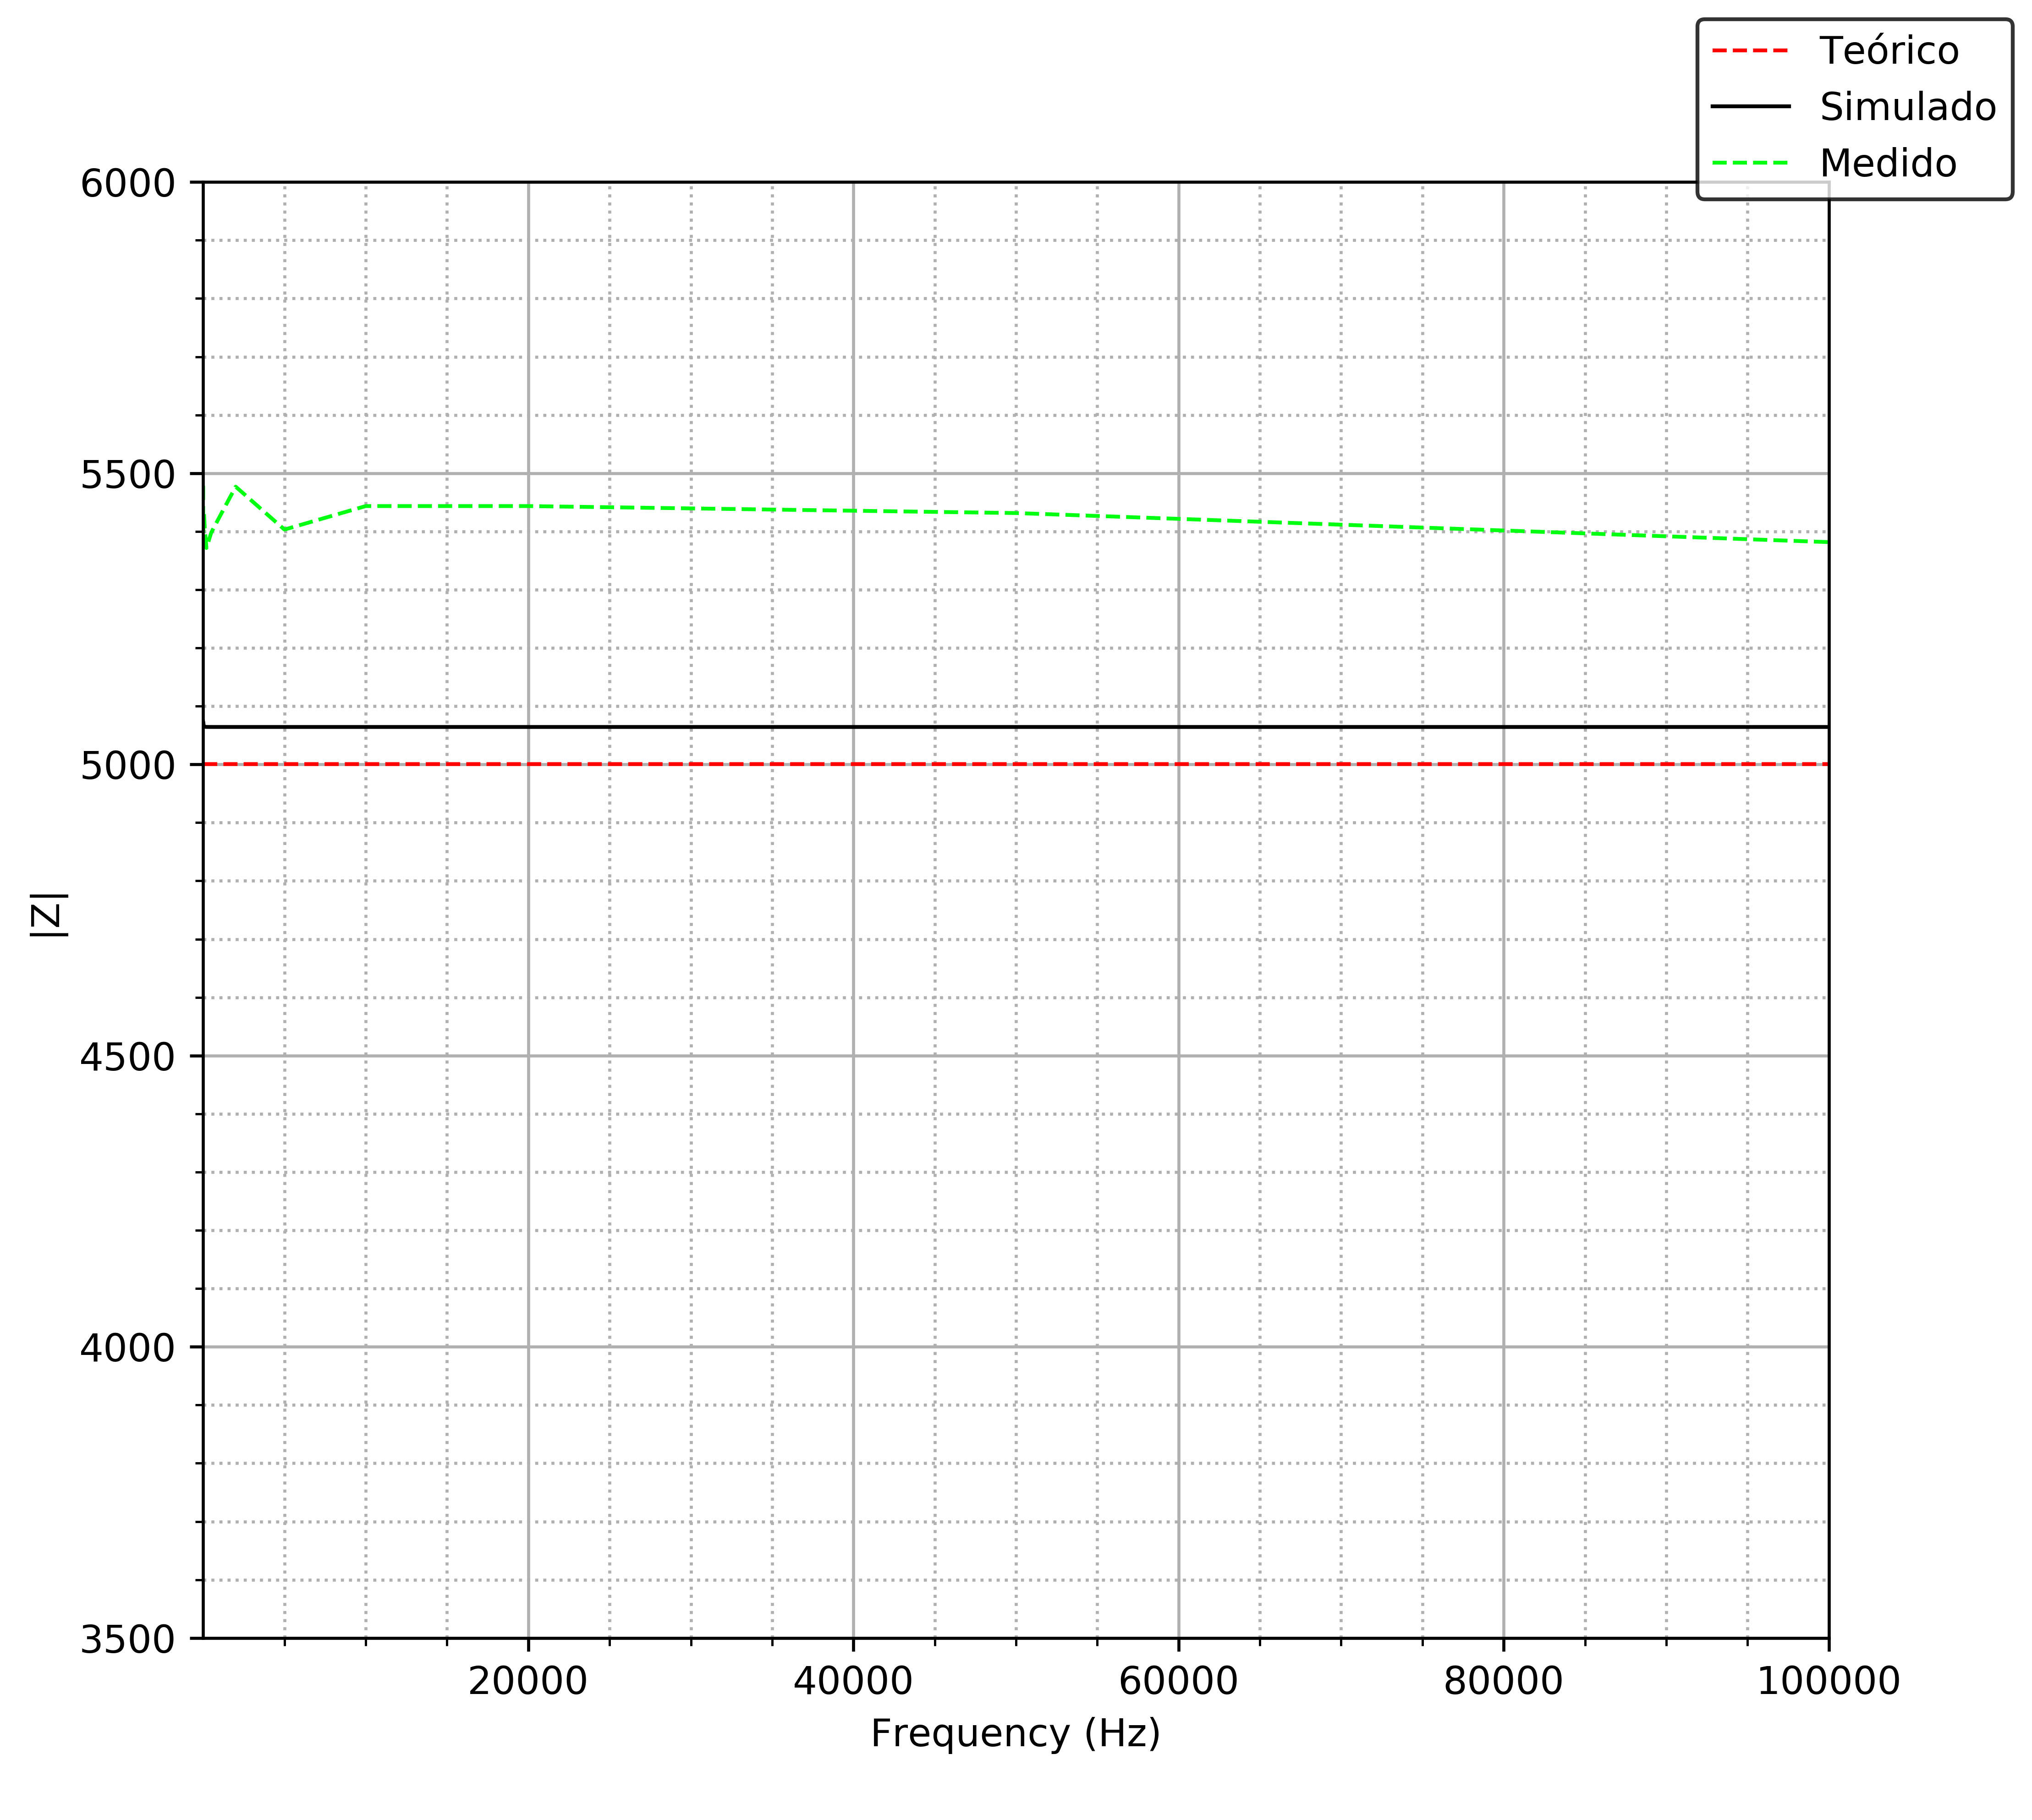
\includegraphics[scale=0.6]{Recursos/Integrador_compensado/impedancia_modulo.png}
	\caption{Impedancia de entrada en m\'odulo del circuito integrador compensado}
	\label{fig:integrador_compensado_impedancia_modulo}
\end{figure}

\begin{figure}[H]
	\centering
	\includegraphics[scale=0.6]{Recursos/Integrador_compensado/impedancia_fase.png}
	\caption{Impedacia de entrada en fase del circuito integrador compensado}
	\label{fig:integrador_compensado_impedancia_fase}
\end{figure}

De las comparaciones anteriores se pueden sacar algunas conclusiones sobre el comportamiento del circuito compensado, como el hecho de que la impedancia
de entrada depende, para un amplio rango de frecuencias, de la resistencia $R_1$ en la entrada del circuito. Adem\'as el circuito tiene un comportamiento
resistivo.

\paragraph*{Respuesta a se\~nales no senoidales} se utilizaron como se\~nales de excitaci\'on para el circuito, una cuadrada de $50 \%$ de duty de frecuencia $f = 1kHz$, una
cuadrada de $62 \%$ de duty y frecuencia $f = 10kHz$, una triangular de $50 \%$ de duty y frecuencia $f = 1kHz$ y, finalmente, una triangular de $80 \%$ de duty y frecuencia de 
$f = 1kHz$. Vale mencionar, que la curva amarilla corresponde a la entrada y la verde a la salida.

Durante la realizaci\'on de estas \'ultimas mediciones se observ\' que para se\~nales con valor medio no nulo, se produce que en la salida
hay un nivel de continua consecuencia del promedio de tal entrada.

\begin{figure}[H]
	\centering
	\begin{tabular}{c c}
		\includegraphics[scale=0.2]{Integrador/Mediciones/Osciloscopio/PCB_Compensado/osc_15.png} &
		\includegraphics[scale=0.2]{Integrador/Mediciones/Osciloscopio/PCB_Compensado/osc_16.png} \\
		\includegraphics[scale=0.2]{Integrador/Mediciones/Osciloscopio/PCB_Compensado/osc_23.png} &
		\includegraphics[scale=0.2]{Integrador/Mediciones/Osciloscopio/PCB_Compensado/osc_27.png}
	\end{tabular}
	\caption{Respuestas a se\~nales no senoidales}
	\label{fig:respuestas_integrador_compensado}
\end{figure}

\subsection{Implementaci\'on pr\'actica}
Para la contrastaci\'on emp\'irica del an\'alisis te\'orico y los resultados de las simulaciones es necesario realizar mediciones sobre
<<<<<<< HEAD
la implementaci\'on pr\'actica y real del circuito propuesto, para lo cual se utiliza Altium Designer para dise\~nar en PCB este circuito.
=======
la implementaci\'on pr\'actica y real del circuito propuesto, para lo cual se utiliza Altium Designer para diseñar en PCB este circuito.
>>>>>>> 1c903573e405a1b067e44751a5fd15495a8566b3
Vale mencionar, que la implementaci\'on engloba todos los circuitos propuestos, sean derivadores o integradores, compensados y sin compensar, por ello
se destina una subsecci\'on general para presentarla.

\paragraph*{Esquem\'atico} como bien se mencion\'o en el an\'alisis te\'orico, los valores principales del derivador e integrador fueron establecidos
como requisito inicial $R = 5k \Omega$ y $C = 20nF$ y de ah\'i que para cumplir con dicha condici\'on fueron necesarias conexiones paralelo entre valores
de componentes comerciales para llegar finalmente a lo propuesto. Por otro lado, para poder hacer pruebas con los circuitos compensado y sin compensar, el derivador
tiene una resistencia variable la cual en su estado $R = 0 \Omega$ hace comportarse al circuito de forma no compensada, mientras que por el otro lado el
integrador tiene un conector para conectar y desconectar la rama de compensaci\'on.
Adem\'as, se agregan al circuito puntos de prueba para medir las se\~nales con las puntas del osciloscopio, y se agrega un conector de selecci\'on del circuito
para permitir medir la impedancia de entrada sin tener cargados ambos circuitos en tal puerto. Al circuito se le agregan capacitores de desacople para compensar necesidades de consumo de corriente relativamente elevada durante intervalos
cortos, evitando así caídas en la diferencia de potencial de la alimentaci\'on del circuito integrado.

Finalmente, a diferencia del circuito te\'orico se agregan resistencias en el terminal no inversor del amplificador operacional, de valores \'optimos $R = 5k \Omega$ con el fin
de reducir los efectos de las corrientes de bias sobre la salida para lograr reducir dicha variable en el an\'alisis. No obstante, el efecto de tales resistencia no fue considerado
te\'oricamente porque pueden ser, desde un punto de vista meramente conceptual, agrupadas con la resistencia interna del amplificador operacional con respecto a la cual se vuelven poco apreciables.
Este \'ultimo comentario cae dentro del marco del an\'alisis de alterna realizado, y no considerando la continua para la cual fue puesta la resistencia, dado que en dicho caso si es apreciable.

\begin{figure}[H]
	\centering
	\begin{tabular}{c c}
		\includegraphics[scale=0.62]{Recursos/Altium/Derivador_esquematico.png} &
		\includegraphics[scale=0.65]{Recursos/Altium/Integrador_esquematico.png} \\
		\includegraphics[scale=0.7]{Recursos/Altium/Entradas_salidas_esquematico.png} &
		\includegraphics[scale=0.7]{Recursos/Altium/Puntos_prueba_esquematico.png}
	\end{tabular}
<<<<<<< HEAD
	\caption{Esquem\'atico del dise\~no en Altium}
	\label{fig:altium_sch}
\end{figure}

\paragraph*{Dise\~no PCB} para minimizar el espacio utilizado en el dise\~no del circuito en PCB y dado que la potencia de las resistencias lo permiten, aprovechando la baja tolerancia de algunos
=======
	\caption{Esquem\'atico del diseño en Altium}
	\label{fig:altium_sch}
\end{figure}

\paragraph*{Dise\~no PCB} para minimizar el espacio utilizado en el diseño del circuito en PCB y dado que la potencia de las resistencias lo permiten, aprovechando la baja tolerancia de algunos
>>>>>>> 1c903573e405a1b067e44751a5fd15495a8566b3
componentes en dicha tecnolog\'ia, se utilizan resistencias y capacitores de tecnolog\'ia SMD en encapsulado 0805.

\begin{figure}[H]
	\centering
	\begin{tabular}{c c}
		\includegraphics[scale=0.6]{Recursos/Altium/Placa_OVERLAY.png} &
		\includegraphics[scale=0.6]{Recursos/Altium/Placa_PCB.png} \\
		\includegraphics[scale=0.6]{Recursos/Altium/Placa_3D_OVERLAY.png} &
		\includegraphics[scale=0.6]{Recursos/Altium/Placa_3D_PCB.png} 
	\end{tabular}
<<<<<<< HEAD
	\caption{Dise\~no del PCB en Altium}
=======
	\caption{Diseño del PCB en Altium}
>>>>>>> 1c903573e405a1b067e44751a5fd15495a8566b3
	\label{fig:altium_pcb}
\end{figure}

\paragraph*{Resultado}, finalmente realizando el proceso de transferencia del PCB se obtuvo.

\begin{figure}[H]
	\centering
	\begin{tabular}{c c}
		\includegraphics[scale=0.55]{Recursos/Altium/OVERLAY_Hecho.png} &
		\includegraphics[scale=0.55]{Recursos/Altium/PCB_Hecho.png}
	\end{tabular}
	\caption{Realizaci\'on del PCB}
	\label{fig:hecho}
\end{figure}

Por \'ultimo, como comentario final, el PCB podr\'ia ser mejorado agregandole un label que indique cual posici\'on del jumper de selecci\'on
corresponde al derivador y cual al integrador. Adem\'as podr\'a agregarse al integrador una etapa previa para proteger al circuito de se\~nales que tengan
componente de corriente continua, utilizando un filtro pasaaltos.

\subsection{Conclusiones}
Los circuitos derivador e integrador propuestos poseen limitaciones en funcionamiento para bajas y altas
frecuencias, puesto que el derivador en bajas frecuencia aten\'ua demasiado y para altas frecuencias, antes de que deje de comportarse como derivador, posee limitaci\'on de funcionamiento por
el slew rate del amplificador operacional, mientras que el integrador para bajas frecuencias tiene alta ganancia y es susceptible a saturar el amplificador operacional, mientras que para altas frecuencias,
antes de que deje de comportarse como integrador, posee una muy alta atenuaci\'on de la se\~nal.

Por otro lado, luego del estudio de estos dos circuitos se ve la importancia de la comparaci\'on del modelo ideal con el modelo no ideal con la menor
cantidad de aproximaciones posible, puesto que este \'ultimo revela para que rango de operaci\'on se puede considerar v\'alido el modelo ideal, y por ende,
el comportamiento que se espera del circuito. Dicho en otras palabras, para los circuitos derivadores e integradores el comportamiento puramente derivador o integrador
se observa en el modelo ideal, no obstante, viendo el modelo m\'as amplio se puede analizar para que rango vale dicho comportamiento. Adem\'as, es de gran importancia
tener en cuenta la impedancia de entrada del circuito a la hora de analizar correctamente los resultados obtenidos, puesto que juega un papel importante cuando tenemos en cuenta
la forma en que se arman y conectan los sistemas que se modelizan.

\end{document}
